\documentclass{LIKE}

\definecolor{MainGreen}{RGB}{22, 160, 133}
\definecolor{MainPurple}{RGB}{142, 68, 173}
\definecolor{MainYellow}{RGB}{211, 84, 0}
\definecolor{MainBlue}{RGB}{41, 128, 185}
\definecolor{MainRed}{RGB}{192, 57, 43}
\definecolor{MainBlack}{RGB}{44, 62, 80}

\begin{document}

\vfill
\begin{tikzpicture}[remember picture, overlay]
    \node[anchor=north west, inner sep=0] at (current page.north west) {%
        
\includegraphics[width=\paperwidth, height=\paperheight]{asset/cover1.png} 
    };

    \fill[JungleGreen] 
        (current page.north east) rectangle ++(-8.0cm, -12.0cm);
    
    %\coordinate (topright) at ([xshift=-2cm, yshift=-5cm]current page.north east);
    \fill[white] 
        ([xshift=-2cm, yshift=-5cm]current page.north east) rectangle ++(-6.0cm, -7.0cm); 

    % “大学物理”大字
    \node[font=\fontsize{64}{64}\selectfont\bfseries, anchor=center] 
        at ([xshift=-5cm, yshift=-6.8cm]current page.north east) {大学};
    \node[font=\fontsize{64}{64}\selectfont\bfseries, anchor=center] 
        at ([xshift=-5cm, yshift=-9.3cm]current page.north east) {物理};

    \fill[brown!90!black] 
        ([xshift=-2cm, yshift=-12cm]current page.north east) rectangle ++(-6.0cm, -2.5cm);
        
    \node[font=\fontsize{18}{22}\selectfont\sffamily\bfseries, Gray, anchor=center] 
        at ([xshift=-5cm, yshift=-11.2cm]current page.north east) {必修~1};
    \node[font=\fontsize{24}{24}\selectfont\bfseries, black, anchor=center] 
        at ([xshift=-5cm, yshift=-13.25cm]current page.north east) {力学~振动与波};

    \node[font=\fontsize{12}{14}\selectfont, text=black, anchor=center] 
        at ([xshift=-5cm, yshift=-2.8cm]current page.north east) {大~学~课~程~自~编~讲~义};
        
    \node[font=\fontsize{14}{14}\selectfont\sffamily\bfseries, text=white, anchor=center] 
        at ([xshift=3cm, yshift=2cm]current page.south west) {张云翼~~编};
\end{tikzpicture}

\colorlet{maincolor}{Black}
\colorlet{sidecolor}{Black!50}

\frontmatter
\setcounter{tocdepth}{1}
\begin{center}
    \renewcommand{\baselinestretch}{1.25}\normalsize
        \tableofcontents
    \renewcommand{\baselinestretch}{1.0}\normalsize
\end{center}

\mainmatter

%\newpage

\colorlet{maincolor}{MainGreen}
\colorlet{sidecolor}{MainGreen!50}

\part{力学}

\chapter{质点运动学}
\setcounter{example_counter}{1}

\section{运动学的物理量}

\subsection{位置矢量、轨道}

\subsubsection{位置矢量}

\noindent
\begin{minipage}{0.74\linewidth}
\setlength{\parindent}{2em}
\setlength{\parskip}{0.5em}
\linespread{1.3}
\textbf{位置矢量}:从原点O指向质点位置P的矢量，用$\vec{r}$表示，简称“位矢”。

在直角坐标中，可用三个坐标值$x,y,z$随时间$t$的变化表示质点的运动。

记$\hat{i},\hat{j},\hat{k}$表示$x,y,z$方向的单位向量，则坐标为$(x,y,z)$的质点，位置矢量可表示为

\begin{formula}
    $\vec{r}=x\hat{i}+y\hat{j}+z\hat{k}$
\end{formula}

\end{minipage}
\hfill
\begin{minipage}{0.25\textwidth}
    \vspace{-1em}
    \centering 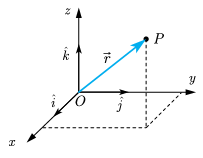
\includegraphics[width=\textwidth]{asset/ch1/T1.png}
\end{minipage}

\subsubsection{轨道}

\textbf{轨道}：质点运动时所经过的路线。只需将$t$消掉，求出$x,y,z$之间的关系。

\begin{example}{求轨道方程}

    根据运动函数求轨道方程：(1)~$\vec{r}=t^2\hat{i}+(2t+3)\hat{j}$ (SI)；(2)~$\vec{r}=\cos^3{t}\hat{i}+\sin^3{t}\hat{j}$ (SI)。
    
    \tcblower

    (1)~根据运动函数，对照$\vec{r}=x\hat{i}+y\hat{j}+z\hat{k}$，可以写出$x=t^2,~y=2t+3$

    \vspace{0.25em}

    根据$y=2t+3$，可以解出$t=\dfrac{(y-3)}{2}$，再代入$x=t^2$，得$x=\dfrac{(y-3)^2}{4}$

    \vspace{0.25em}

    整理得$4x=(y-3)^2$，这就是质点的轨道方程。注：若只考虑$t\geq 0$的运动，则还应有$y\geq 3$.

    (2)~根据运动函数，可写出$x=\cos^3{t},~y=\sin^3{t}$

    利用$\cos^2{t}+\sin^2{t}=1$，可配凑出$x^{\frac{2}{3}}+y^{\frac{2}{3}}=1$，这就是质点的轨道方程。

    \tcbline

    \noindent
    \begin{minipage}{0.78\linewidth}
    \setlength{\parskip}{0.5em}
    \linespread{1.3}
    【补充练习】质点做初速度斜向上$45^\circ$的斜抛运动，坐标系如图所示。根据斜抛运动规律，写出$x,y$随$t$的变化关系，并求质点的轨道方程。
    \end{minipage}
    \hfill
    \begin{minipage}{0.2\textwidth}
        \centering 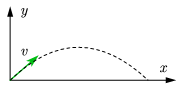
\includegraphics[width=\textwidth]{asset/ch1/T2.png}
    \end{minipage}
    
\end{example}

\subsection{位移与路程}

%\subsubsection{定义}

\noindent
\begin{minipage}{0.83\linewidth}
\setlength{\parskip}{0.5em}
\setlength{\parindent}{2em}
\linespread{1.3}

\textbf{路程}：质点运动的路径长，记为$\Delta s$，路程是标量，只有大小，没有方向。

\textbf{位移}：质点位置的改变量，记为$\Delta \vec{r}$，位移是矢量，既有大小，也有方向。

\warn{在大学物理中，矢量上方的箭头不可省略，位移不能写成$\Delta r$.}
\end{minipage}
\hfill
\begin{minipage}{0.15\textwidth}
    \vspace{-1em}
    \centering 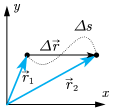
\includegraphics[width=\textwidth]{asset/ch1/T3.png}
\end{minipage}

%\subsubsection{关系}

因为两点之间，直线段最短，所以路程不小于位移的大小。$\Delta s \geq |\Delta \vec{r}|$

但时间$\Delta t \rightarrow 0$时，任意曲线运动可近似为直线运动，$ds = |d \vec{r}|$

\note{当时间足够短，$\Delta t \rightarrow 0$时，$\Delta$符号可改写为$d$符号。}

\warn{若矢量不写箭头，则认为是矢量的大小，$r$表示的是$|\vec{r}|$. 在大学物理阶段，$\Delta |\vec{r}|$、$\Delta r$、$d |\vec{r}|$、$dr$这些写法都是错误的，没有物理意义。位移的大小必须写成$|\Delta \vec{r}|$、$|d \vec{r}|$.}

\subsection{速度与速率}

\subsubsection{速度}

速度是位置的变化率，是单位时间内的位移，是矢量，既有大小，也有方向。

平均速度等于位移除以时间，$\bar{\vec{v}}=\dfrac{\Delta \vec{r}}{\Delta t}$，$\Delta t \rightarrow 0$时的极限，即为瞬时速度$\vec{v}=\dfrac{d\vec{r}}{dt}$

在直角坐标中，可以对三个坐标分别求导，得到速度在三个方向上的分量。

\begin{formula}
    $\vec{v}=\dfrac{d\vec{r}}{dt}=\dfrac{dx}{dt}\hat{i}+\dfrac{dy}{dt}\hat{j}+\dfrac{dz}{dt}\hat{k}$
\end{formula}

\subsubsection{速率}

速率是单位时间内的路程，是标量，只有大小，没有方向。

平均速率等于路程除以时间，$\bar{v}=\dfrac{\Delta s}{\Delta t}$，$\Delta t \rightarrow 0$时的极限称为瞬时速率$v=\dfrac{ds}{dt}$

\subsubsection{速度与速率的关系}

因为$\Delta s \geq |\Delta \vec{r}|$，所以平均速率不小于平均速度的大小。

但是$ds = |d \vec{r}|$，所以瞬时速率等于瞬时速度的大小。

\begin{example}{速度与速率的定义}
    质点在$xy$平面上运动。下列写法中，哪些表示瞬时速度，哪些表示瞬时速率？

    \vspace{0.3em}

    A. $\dfrac{d \vec{r}}{dt}$~~~B. $\dfrac{d |\vec{r}|}{dt}$~~~C. $\dfrac{dr}{dt}$~~~D. $\left|\dfrac{d\vec{r}}{dt}\right|$~~~E. $\dfrac{ds}{dt}$~~~F. $\dfrac{dx}{dt}+\dfrac{dy}{dt}$~~~G. $\sqrt{\left(\dfrac{dx}{dt}\right)^2+\left(\dfrac{dy}{dt}\right)^2}$

    \tcblower

    A是瞬时速度的定义，E是瞬时速率的定义，D是瞬时速度的大小，表示瞬时速率。
    
    B和C出现了$d |\vec{r}|$、$dr$的错误写法，无物理意义。

    \vspace{0.3em}

    $\dfrac{dx}{dt}$、$\dfrac{dy}{dt}$分别表示速度在$x,y$方向的分量$v_x,v_y$，合成时应采用勾股定理，而非直接相加。

    \vspace{0.3em}
    
    因此G选项表示瞬时速率，F选项无物理意义。

    \tcbline

    【补充练习】质点做半径为$R$的匀速圆周运动，周期为$T$，求$t=2T$时间内的位移、路程、平均速度、平均速率。
    
\end{example}

\subsection{加速度}

加速度是速度的变化率，也可分为平均加速度和瞬时加速度。

平均加速度等于速度的变化量除以时间，$\overline{\vec{a}}=\dfrac{\Delta \vec{v}}{\Delta t}$，$\Delta t \rightarrow 0$时的极限称为瞬时加速度$\vec{a}=\dfrac{d\vec{v}}{dt}$

在直角坐标系中，分别对$x,y,z$求二阶导（即两次求导），得到的就是加速度在三个方向上的分量。

\begin{formula}
    $\vec{a}=\dfrac{d\vec{v}}{dt}=\dfrac{d^2\vec{r}}{dt^2}=\dfrac{d^2x}{dt^2}\hat{i}+\dfrac{d^2y}{dt^2}\hat{j}+\dfrac{d^2z}{dt^2}\hat{k}$
\end{formula}


\begin{itemize}
    \item 对于直线运动而言，速度与加速度同向时加速，反向时减速。不是加速度为正时加速，为负时减速。
    \item 对于曲线运动，速度与加速度夹角小于$90^\circ$时加速，大于$90^\circ$时减速。
\end{itemize}

\subsection{运动学的两类基本问题}

位置矢量$\vec{r}$、速度$\vec{v}$、加速度$\vec{a}$的关系如下。知道一个物理量随时间的关系，即可求出另外两个。

\note{如无特殊说明，速度、加速度默认都是指瞬时速度、加速度。}

\begin{figure}[htb]
    \centering
    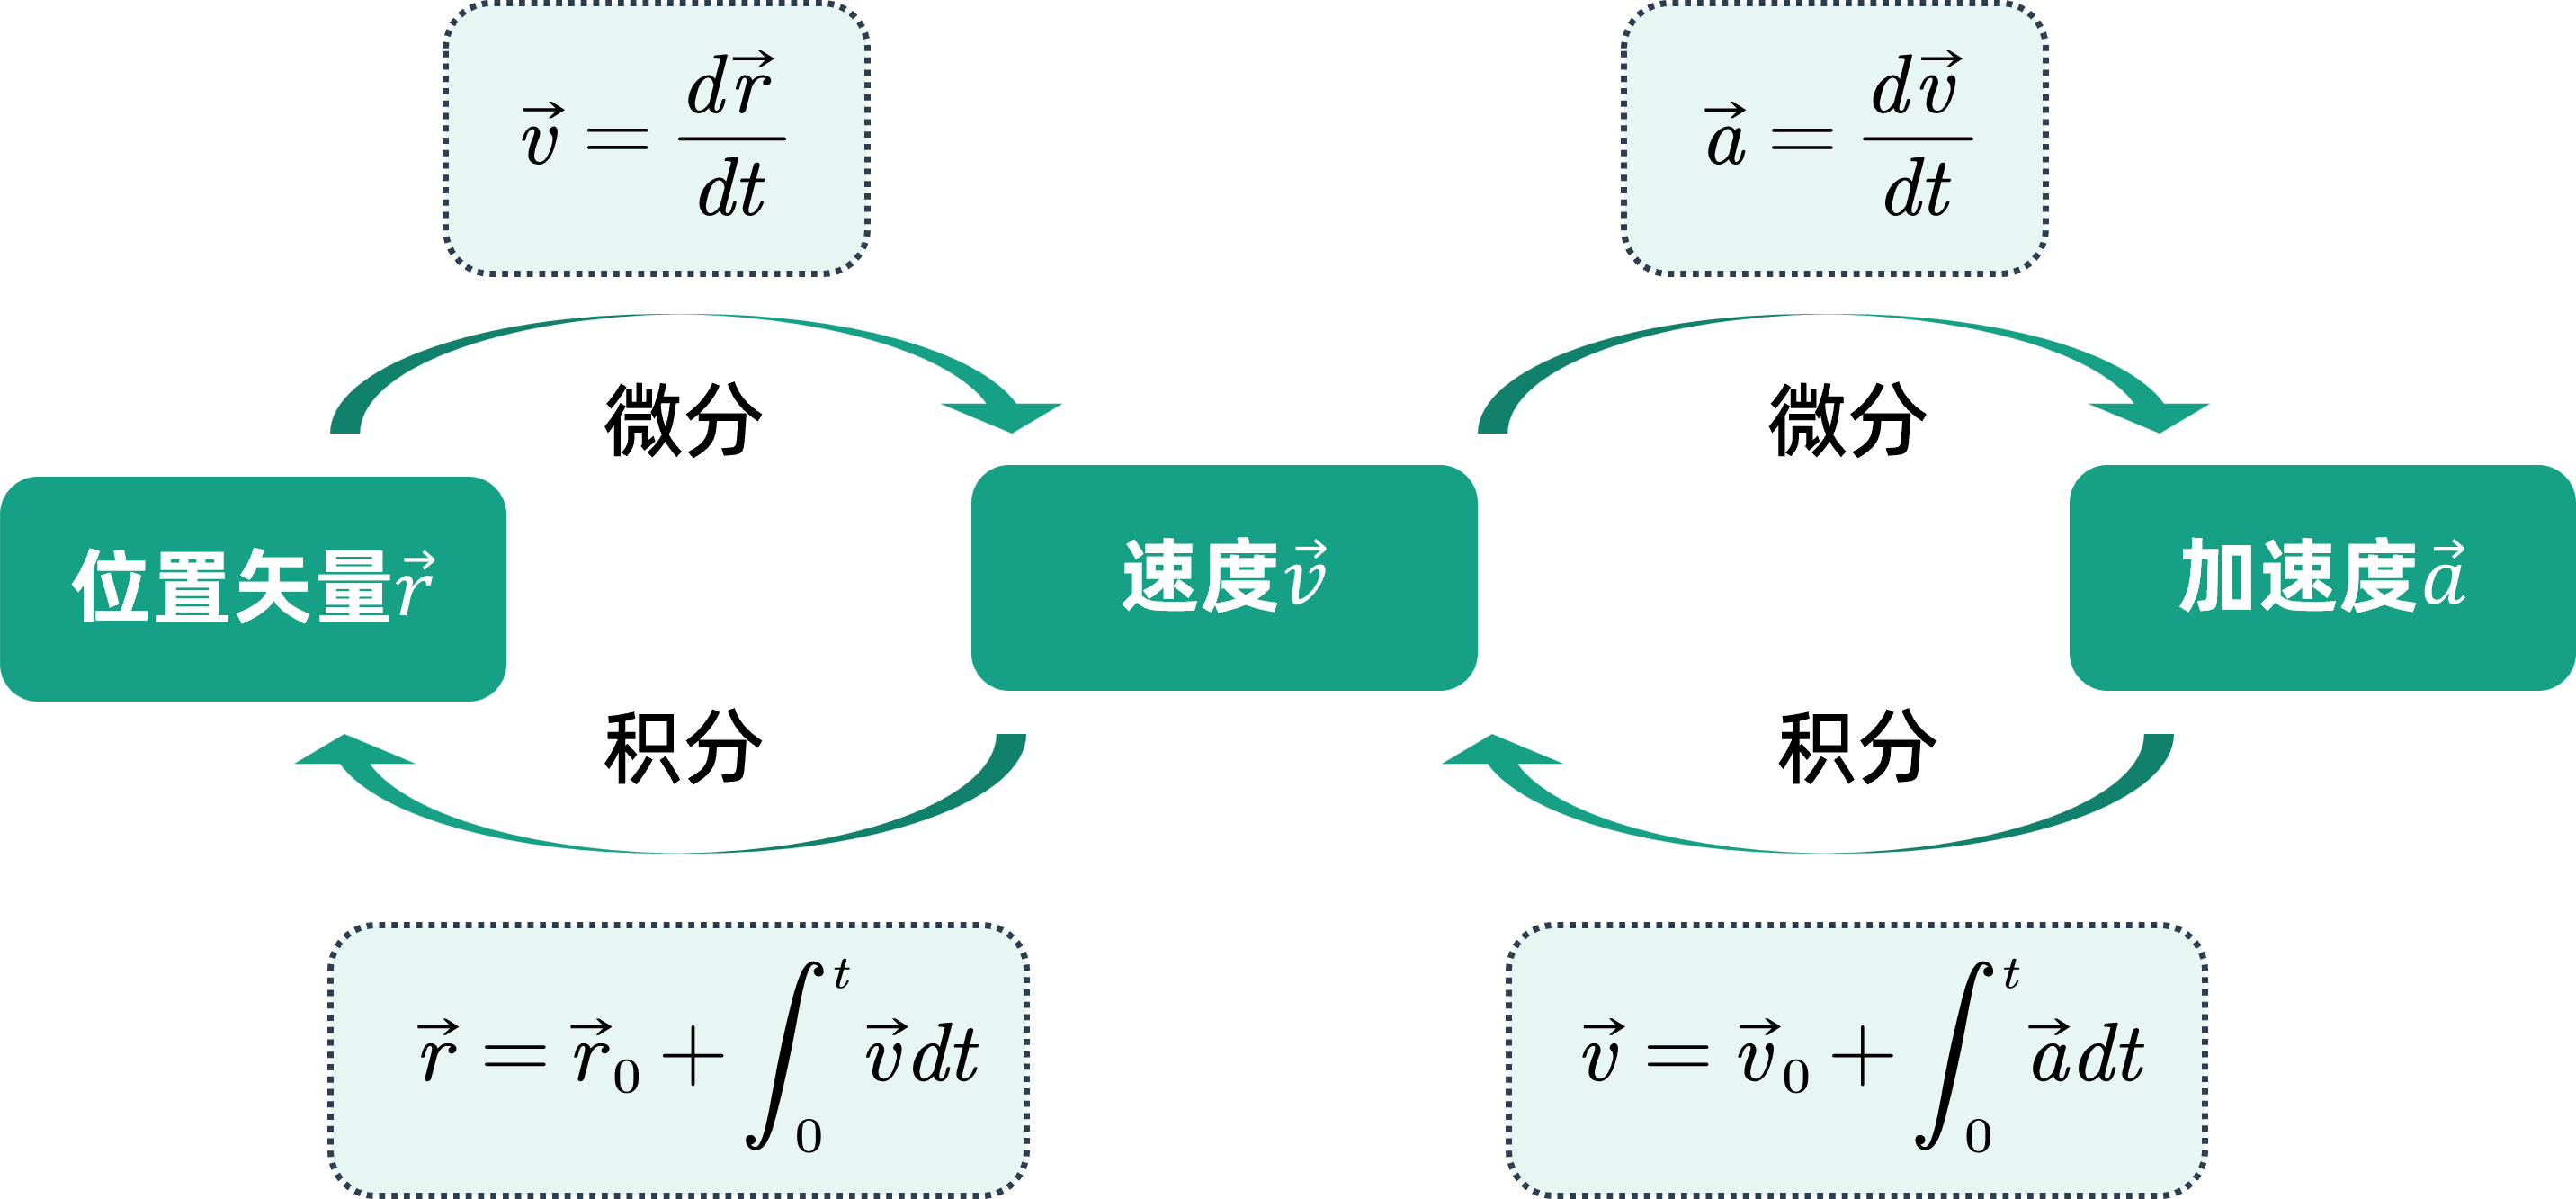
\includegraphics[width=0.65\linewidth]{asset/ch1/T4.png}
\end{figure}

\warn{注意在积分求解时，不要忘了考虑初始条件。}

\begin{example}{运动学第一类问题}
    运动函数为$\vec{r}=(3t+5)\hat{i}+(t^2+3t−4)\hat{j}$(SI)，求：$t=\SI{4}{s}$时的速度和加速度，前$\SI{4}{s}$的平均速度。

    \tcblower

    根据质点运动函数，可写出$x=3t+5,~y=t^2+3t−4$

    \vspace{0.25em}
    
    求导可得$v_x=\dfrac{dx}{dt}=3,~v_y=\dfrac{dy}{dt}=2t+3$，再次求导可得$a_x=\dfrac{d^2x}{dt^2}=0,~a_y=\dfrac{d^2y}{dt^2}=2$

    \vspace{0.3em}

    将$t=\SI{4}{s}$，代入，可得$v_x=3,~v_y=11,a_x=0,~a_y=2$，可写成$\vec{v}=3\hat{i}+11\hat{j},~\vec{a}=2\hat{j}$

    要求平均速度，需要先求位移。当$t=0,\SI{4}{s}$时，$\vec{r}_1=5\hat{i}-4\hat{j},~\vec{r}_2=17\hat{i}+24\hat{j}$

    \vspace{0.3em}

    所以位移$\Delta \vec{r}=\vec{r}_2-\vec{r}_1=12\hat{i}+28\hat{j}$，平均速度$\bar{\vec{v}}=\dfrac{\Delta \vec{r}}{\Delta t}=3\hat{i}+7\hat{j}$
    
    \tcbline
    【补充练习】已知质点运动方程为$x=2t,~y=2-t^2$，求：(1)~前$\SI{2}{s}$内的平均速度、第$\SI{2}{s}$末的速度；(2)~前$\SI{2}{s}$内的平均加速度、第$\SI{2}{s}$末的加速度。
\end{example}

\begin{example}{运动学第二类问题}
    质点沿$x$轴运动，加速度$a=-6t$~(SI)。已知$t=\SI{3}{s}$时，$x=\SI{-12}{m},~v=\SI{-24}{m/s}$，求： (1)~求任意时刻的速度和位置；(2)~判断什么时候向正方向运动，什么时候向负方向运动（只考虑$t\geq 0$）；(3)~判断什么时候加速、什么时候减速；(4)~求前$\SI{2}{s}$内的路程、位移、平均速度、平均速率。

    \tcblower

    (1)~~将$a$对$t$求积分，可得$v=v_0+\displaystyle \int_0^t{(-6t)dt}=v_0-3t^2$

    \vspace{0.25em}
    
    代入$t=3$时$v=-24$，得$v_0=3$，因此$v=3-3t^2$

    \vspace{0.25em}

    再将$v$对$t$求积分，可得$x=x_0+\displaystyle \int_0^t{(3-3t^2)dt}=x_0+3t-t^3$

    \vspace{0.25em}
    
    代入$t=3$时$x=-12$，得$x_0=6$，因此$x=3t-t^3+6$
    \note{在一维问题中，矢量运算退化成标量运算，可省略上方的箭头，用正负表示其方向。}

    (2)~~当$v>0$时，即$0\leq t<\SI{1}{s}$时，向正方向运动；而$v<0$时，即$t>\SI{1}{s}$时，向负方向运动。

    (3)~~因为$a=-6t<0$，因此当$0\leq t<\SI{1}{s}$时，$v>0$，加速度与速度反向，为减速；
    
    而$t>\SI{1}{s}$时，$v<0$，加速度与速度同向，为加速。

    (4)~~当$t=0,\SI{1}{s},\SI{2}{s}$时，代入表达式可求出$x=\SI{6}{m},\SI{8}{m},\SI{4}{m}$

    位移就是位置变化量，只看初末状态即可，$\Delta x=\SI{4}{m}-\SI{6}{m}=\SI{-2}{m}$

    路程需要按转向时刻分段求解，第$\SI{1}{s}$路程为$\SI{2}{m}$，第$\SI{2}{s}$路程为$\SI{4}{m}$，因此总路程为$\SI{6}{m}$

    平均速度等于位移除以时间，等于$\SI{-1}{m/s}$；平均速率等于路程除以时间，等于$\SI{3}{m/s}$.

    \tcbline
    【补充练习】质点从$\vec{r}=−5\hat{j}$处出发，初速度$\vec{v}=2\hat{i}$。加速度与时间的关系为$\vec{a}=t^2\hat{i}+(2t+3)\hat{j}$(SI)，求：质点在$t=\SI{2}{s}$时的速度和位置矢量。
\end{example}

\section{圆周运动}

\subsection{圆周运动的描述}

在圆周运动中，我们更关心转过角度的变化，因此可以将位置、速度、加速度推广为角位置$\theta$、角速度$\omega$、角加速度$\alpha$，它们之间的微分、积分关系完全相同。

\begin{figure}[htb]
    \centering
    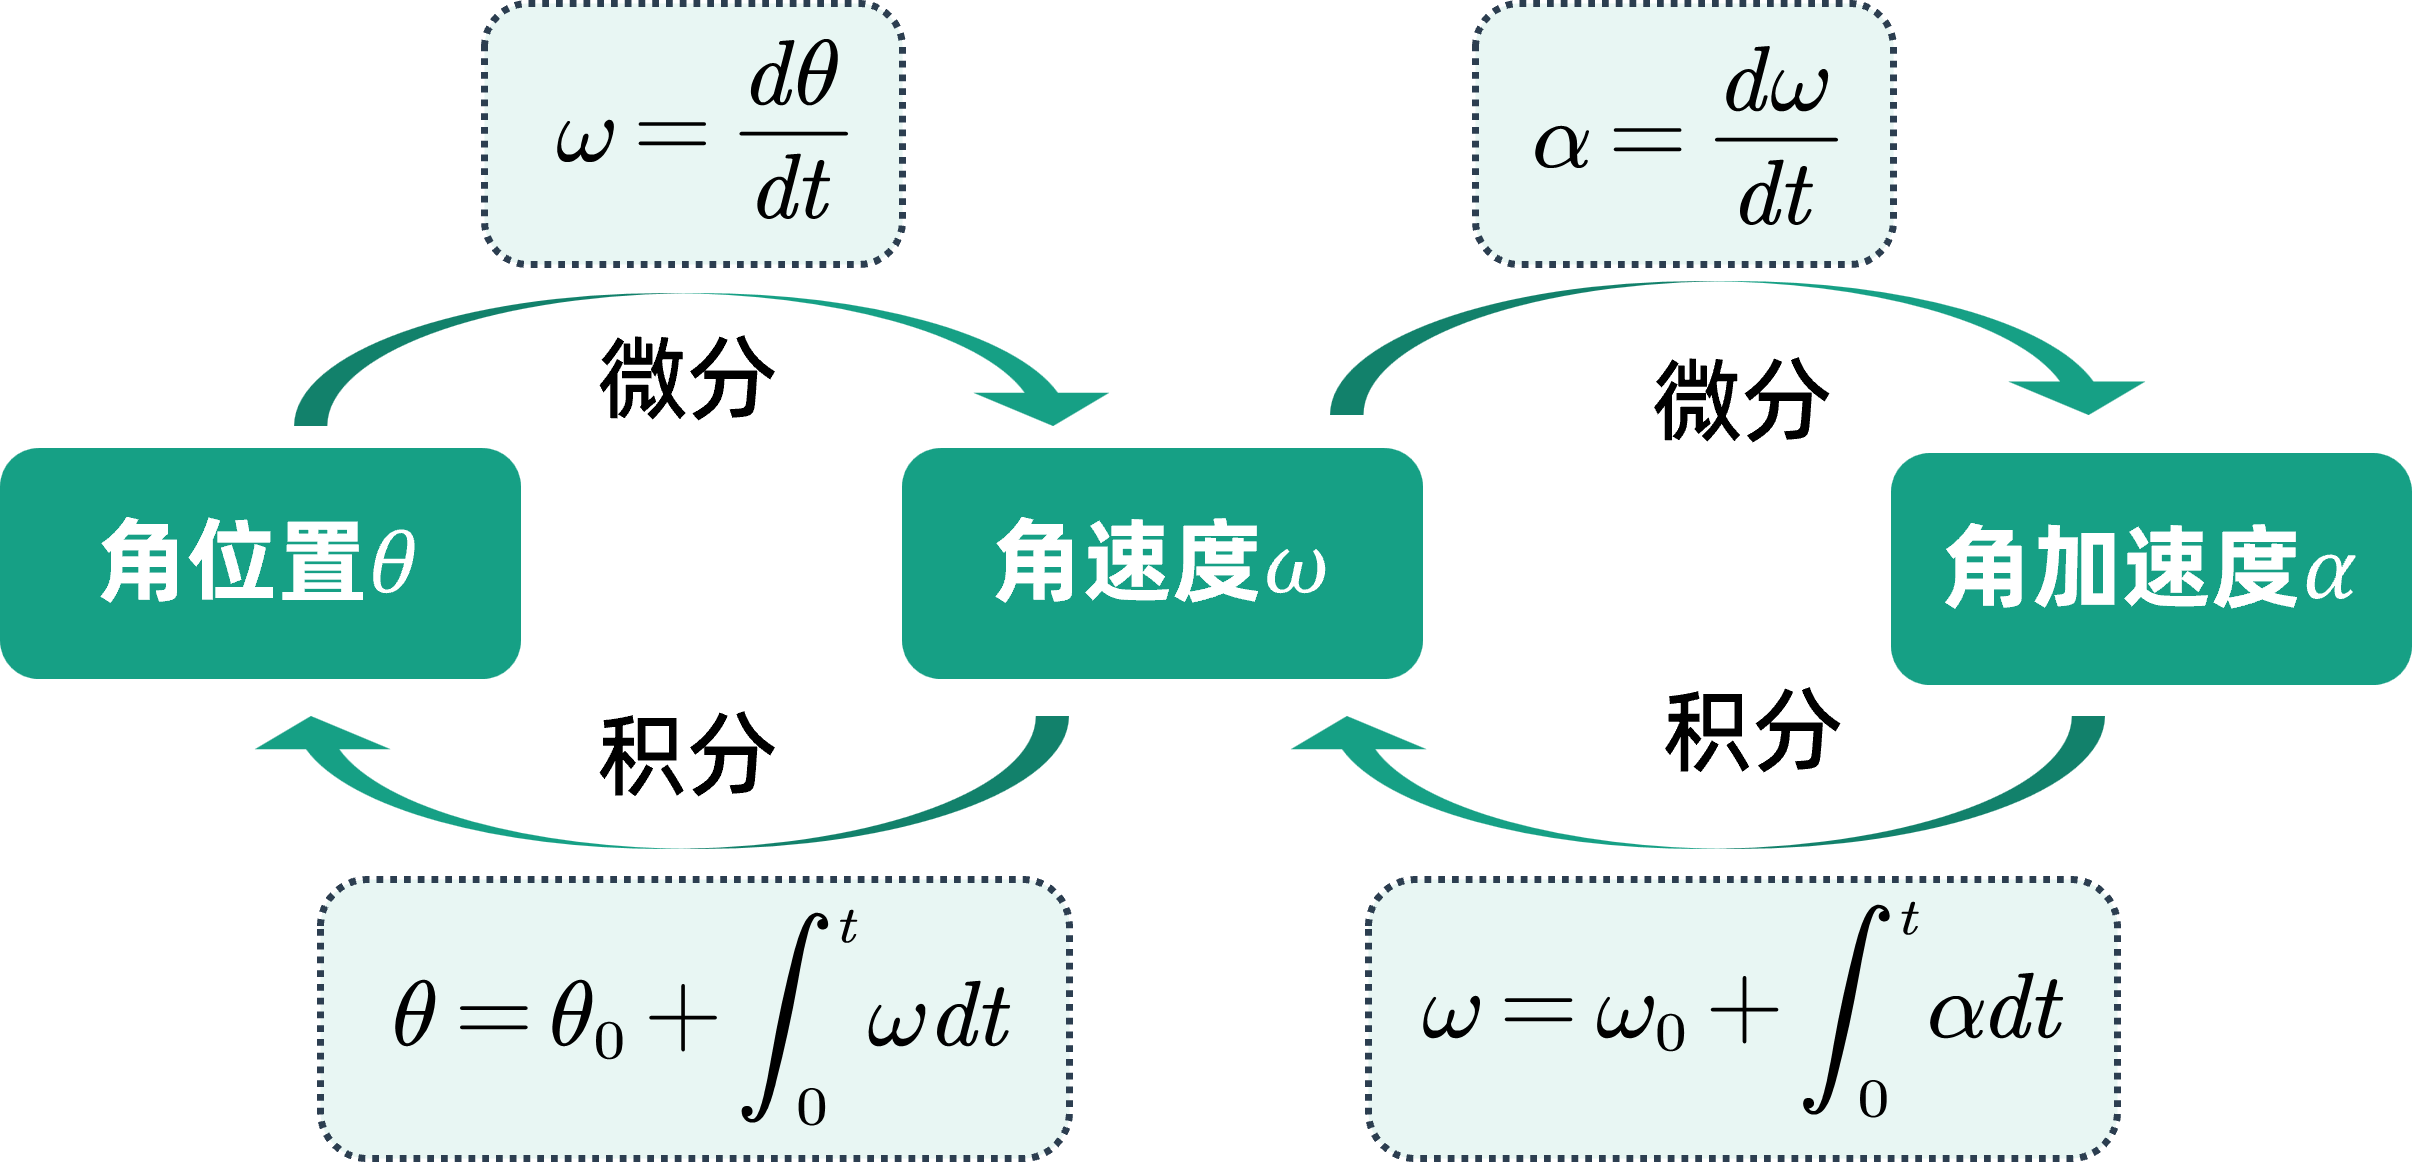
\includegraphics[width=0.65\linewidth]{asset/ch1/T8.png}
\end{figure}

\note{一些教材将角加速度记为符号$\beta$，但国家标准规定为$\alpha$.}

\note{角速度$\omega$是矢量，方向用右手螺旋判断，但大学物理不强调其矢量性。}

%\begin{formula}
%    $\omega=\dfrac{d\theta}{dt},~\alpha=\dfrac{d\omega}{dt},~\theta=\theta_0+\displaystyle\int_0^t{\omega dt},~\omega=\omega_0+\displaystyle\int_0^t{\alpha dt}$
%\end{formula}

\subsection{线量与角量的关系}

路程$s$与角位移$\theta$、线速度$v$与角速度$\omega$的换算只需乘除一个半径$R$，速度的方向为切线方向。

\begin{formula}
    $s=\theta R,~v=\dfrac{ds}{dt}=\omega R$
\end{formula}

但加速度$a$需要分解为切向和法向分别计算：

\begin{itemize}
    \item 切向加速度$a_t$：控制速度大小的变化，是速率的变化率，与速度同向时加速，反向时减速
    \item 法向加速度$a_n$：控制速度方向的变化，指向圆心，即向心加速度
\end{itemize}

%切向与法向加速度的定量表达式为：

\begin{formula}
    $a_t=\dfrac{dv}{dt}=\alpha R,~a_n=\dfrac{v^2}{R},~a=\sqrt{a_t^2+a_n^2}$
\end{formula}

\warn{注意求加速度时，一定要分别求出两个分量，再做合成，而不能直接用角加速度乘以半径。}

\begin{example}{圆周运动}
    质点做$R=2$的圆周运动，静止出发，角加速度与时间的关系为$\alpha=12t^2−6t$（SI）
    
    (1) 求任意时刻的角速度、角位移；(2) 求$t=2$时刻的线速度和加速度的大小。
    \tcblower
    
    (1)~静止出发可知初始$\omega_0=0$，对角加速度积分可得角速度，$\omega=0+\displaystyle\int_0^t{(12t^2-6t)dt}=4t^3-3t^2$

    %\vspace{0.25em}

    再求一次积分，即可得到角位移
    $\theta=0+\displaystyle\int_0^t{(4t^3-3t^2)dt}=t^4-t^3$

    \vspace{0.25em}

    (2)~代入$t=2$，可得$\alpha=36,~\omega=20$，根据线量与角量的关系，$v=\omega R=40$

    \vspace{0.25em}

    加速度需要分别求切向和法向，$a_t=\alpha R=72,~a_n=\dfrac{v^2}{R}=800$，合成可得$a=\sqrt{a_t^2+a_n^2}\approx 803$
    \tcbline
    【补充练习】质点做$R=3$的圆周运动，路程与时间的关系为$s=3t+3t^2$，始终逆时针运动。(1)~求$t=2$时刻的线速度、角速度、加速度、角加速度的大小；(2)~在哪一时刻，加速度与速度方向的夹角为$45^\circ$？
\end{example}

\section{相对运动}

仅考虑参考系相对于大地平动的情况，变换参考系前后，可定义三种速度：
\begin{itemize}
    \item \textbf{绝对速度}：质点相对于大地的速度
    \item \textbf{相对速度}：质点相对于选定参考系的速度
    \item \textbf{牵连速度}：选定参考系相对于大地的速度
\end{itemize}

这三种速度之间的关系是

\begin{formula}  
   $\text{绝对}=\text{相对}+\text{牵连}$
\end{formula}


\note{上式的加法应理解为矢量相加，位移、加速度也满足类似的关系。}

\begin{example}{相对运动}
    某人以速度$v$向西匀速骑车，有风从北偏东$30^\circ$方向以相同速率吹来，这个人感受到的风来自什么方向，风速如何？
    \tcblower

    空气流动产生了风，以空气为研究对象，风的速度是空气相对于大地的速度，是绝对速度。

    \vspace{0.7em}

    \noindent
    \begin{minipage}{0.78\linewidth}
    \setlength{\parskip}{0.5em}
    \linespread{1.1}
    
    而人感受到的风，应是空气相对于人的速度，是相对速度。

    此时，参考系应变换到人的身上，因此人相对于大地的速度是牵连速度。

    根据题意，结合绝对=相对+牵连的关系，可画出三者之间的关系如右图所示。因此人感受到的风，即相对速度，为北偏西$30^\circ$方向，大小为$v$.
    \end{minipage}
    \hfill
    \begin{minipage}{0.2\textwidth}
        \centering 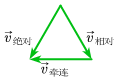
\includegraphics[width=\textwidth]{asset/ch1/T10.png}
    \end{minipage}
    
    \tcbline
    【补充练习】以正东、正北为$x,y$轴正方向。甲乙两船以$\SI{2}{m/s}$的速率匀速行驶，甲向正东方向运动，乙向北偏东$30^\circ$方向运动。求乙相对于甲的速度。
\end{example}

\section{拓展内容}

\subsection{运动学的实际问题}

在一个实际场景中，要求某点的速度或加速度，可建立坐标系，利用该点的坐标建立几何关系，再对等号两边同时求导，即可得到未知点与已知点之间的速度、加速度关系。

\note{注意$x,y$是时间的函数，求导时要用隐函数求导法则。例如$x^2$求导的结果不是$2x$，而是$2x\dfrac{dx}{dt}$.}

\begin{example}{运动学实际问题*}
    一人通过岸边的定滑轮（大小可忽略）用绳子拉船，使船靠岸，假定绳子不可伸长且始终绷紧，拉绳的速率恒为$u$，水面与滑轮的高度差为$H$.~求当绳与水平面夹角为$\theta$时，船运动的速度和加速度。
    \tcblower
    
    \noindent
    \begin{minipage}{0.73\linewidth}
    \setlength{\parskip}{0.5em}
    \linespread{1.3}
    建立如图所示的坐标系，设船的横坐标为$x$，滑轮到船之间的绳长为$L$
    
    则根据勾股定理，$x^2+H^2=L^2$，根据题意，绳缩短的速率$\dfrac{dL}{dt}=-u$

    {\fangsong 注：$\dfrac{dL}{dt}=-u$并不表示某一质点的速度，而是绳长对时间的变化率}

    \vspace{-0.1em}

    \end{minipage}
    \hfill
    \begin{minipage}{0.25\textwidth}
        \centering 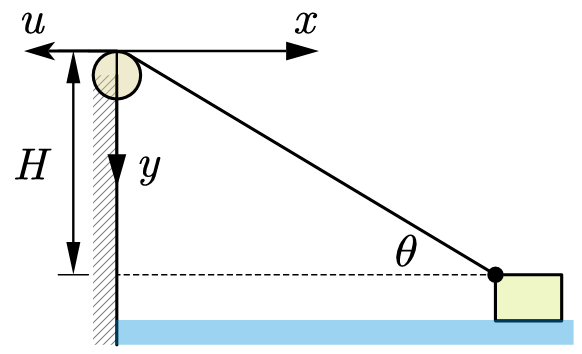
\includegraphics[width=\textwidth]{asset/ch1/T12.png}
    \end{minipage}

    对两边分别求导得$2x\dfrac{dx}{dt}+0=2L\dfrac{dL}{dt}$，解得$v=\dfrac{dx}{dt}=-\dfrac{L}{x}u=-\dfrac{u}{\cos{\theta}}$

    对$x\dfrac{dx}{dt}=L\dfrac{dL}{dt}$两边再求导，得$\left(\dfrac{dx}{dt}\right)^2+x\dfrac{d^2x}{dt^2}=\left(\dfrac{dL}{dt}\right)^2+L\dfrac{d^2L}{dt^2}$

    \vspace{0.3em}

    而其中$\dfrac{d^2L}{dt^2}=0$，代入整理得$a=\dfrac{d^2x}{dt^2}=\dfrac{u^2-v^2}{x}=\dfrac{u^2(1-1/\cos^2\theta)}{H/\tan\theta}=-\dfrac{u^2\tan^3{\theta}}{H}$
    
    \tcbline
    
    \noindent
    \begin{minipage}{0.78\linewidth}
    \setlength{\parskip}{0.5em}
    \linespread{1.3}
    【补充练习】长为$L$的木棍靠在墙上，慢慢滑落。记木棍下端为A点、上端为B点，假设A点的移动速度恒为$v$。某一时刻，木棍与水平方向夹角为$\theta$。求B点此时的速度和加速度。
    \end{minipage}
    \hfill
    \begin{minipage}{0.2\textwidth}
        \centering 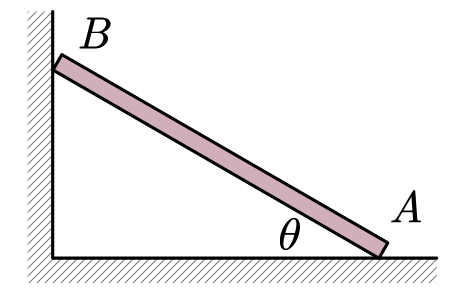
\includegraphics[width=\textwidth]{asset/ch1/T6.png}
    \end{minipage}
\end{example}

\subsection{曲线运动与自然坐标系}

\noindent
    \begin{minipage}{0.73\linewidth}
    
    \setlength{\parskip}{0.5em}
    \setlength{\parindent}{2em}
    \linespread{1.3}
    \subsubsection{自然坐标系}

    \vspace{1em}
    
    若质点做曲线运动，可沿轨道建立坐标系，选定原点O后，用曲线长度$s$表示质点的位置，这种坐标系称为\textbf{自然坐标系}。
    \end{minipage}
    \hfill
    \begin{minipage}{0.25\textwidth}
        \centering 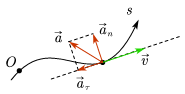
\includegraphics[width=\textwidth]{asset/ch1/T7.png}
    \end{minipage}

在任意时刻，速度方向为曲线的切线方向，大小（即速率）等于$v=\dfrac{ds}{dt}$

\subsubsection{曲线运动的加速度}

在曲线运动中，曲线上各点都可以找到一个贴合最好的圆，称为“曲率圆”，其半径称为“曲率半径”，用$\rho$表示。因此，曲线运动的每一小段都可近似为一个圆周运动，从而求出切向和法向加速度。

\begin{itemize}
    \item 切向加速度：控制速度大小的变化，是速率的变化率，$a_t=\dfrac{dv}{dt}$
    \item 法向加速度：控制速度方向的变化，指向曲线凹侧，$a_n=\dfrac{v^2}{\rho}$
\end{itemize}

\warn{注意加速度是速度的变化率，而切向加速度是速率的变化率。}

在自然坐标系下，曲线运动的速度和加速度的定量表达式总结如下。

\begin{formula}
    $v=\dfrac{ds}{dt},~a_t=\dfrac{dv}{dt},~a_n=\dfrac{v}{\rho^2}$
\end{formula}

\begin{example}{自然坐标系*}
    质点以$\SI{10}{m/s}$的速度水平抛出，做平抛运动。当速度方向与水平方向成$60^\circ$角时，求瞬时速率、速度变化率、速率的变化率、曲率半径。（取$g=\SI{10}{m/s^2}$）
    \tcblower
    
    \begin{minipage}{0.78\linewidth}
    
    \setlength{\parskip}{0.5em}
    
    \linespread{1.3}
    根据平抛运动的规律，水平方向做匀速直线运动，因此$v=\dfrac{v_x}{\cos{60^\circ}}=\SI{20}{m/s}$

    \vspace{0.25em}

    速度的变化率就是瞬时加速度，而平抛运动的加速度是重力加速度，大小为$a=g=\SI{10}{m/s^2}$，方向竖直向下，这就是速度的变化率。

    加速度可在平行和垂直速度的方向上进行分解。
    
    切向加速度$a_t=a\sin{30^\circ}=5\sqrt{3}\unit{m/s^2}$，这就是速率的变化率。

    \vspace{0.3em}

    法向加速度$a_n=a\cos{30^\circ}=\SI{5}{m/s^2}$，利用$a_n=\dfrac{v^2}{\rho}$，得曲率半径$\rho=\SI{80}{m}$

    \end{minipage}
    \hfill
    \begin{minipage}{0.2\textwidth}
        \centering 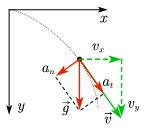
\includegraphics[width=\textwidth]{asset/ch1/T11.png}
    \end{minipage}
    
    \tcbline
    【补充练习】质点运动方程为$x=3t, y=12−3t^2$(SI)，求$t=\SI{1}{s}$时的瞬时速度、速度的变化率、速率的变化率和曲率半径。
\end{example}

\chapter{质点动力学（上）}
\setcounter{example_counter}{1}
\section{牛顿运动定律}

%\subsection{牛顿运动定律的内容}

\begin{itemize}
    \item 牛顿第一定律：任何物体都保持静止或匀速直线运动的状态，除非作用在它上面的力迫使它改变这种状态
    \item 牛顿第二定律：运动的变化与所加的动力成正比，并且发生在这个力所沿的直线方向
    \begin{formula}
        $\vec{F}=\dfrac{d\vec{p}}{dt}=m\dfrac{d\vec{v}}{dt}=m\vec{a}$
    \end{formula}
    \item 牛顿第三定律：两个物体对各自对方的相互作用总是相等的，而且指向相反方向
\end{itemize}

\warn{注意，牛顿运动定律仅在惯性参考系中成立，且仅适用于宏观物体的低速运动。}

%\subsection{牛顿第二定律的应用}

\begin{example}{牛顿第二定律与微积分结合}
    汽艇关掉发动机后，因水面阻力而逐渐减速。设关机后速度为$v_0$，阻力大小为$kv$，汽艇质量为$m$，求$t$时刻的速率和停止前通过的路程。

    \tcblower

    (1)~根据牛顿第二定律，$F=-kv=m\dfrac{dv}{dt}$，分离变量得$\dfrac{dv}{v}=-\dfrac{k}{m}dt$

    \vspace{0.5em}

    两边分别积分$\displaystyle\int{\dfrac{dv}{v}}=-\int{\dfrac{k}{m}dt}$，得$\ln{v}=C-\dfrac{k}{m}t$
    
    \vspace{0.25em}

    初始条件为$t=0$时，$v=v_0$，代入求得$C=\ln{v_0}$. 代回整理得$v=v_0 e^{-\frac{k}{m}t}$

    \vspace{0.25em}

    (2)~位移$x=\displaystyle \int_0^t{v_0 e^{-\frac{k}{m}t}dt}=\dfrac{m}{k}v_0(1-e^{-\frac{k}{m}t})$，
    当$t\rightarrow \infty$时，$x\rightarrow \dfrac{m}{k}v_0$，这就是停止前通过的路程。
   
    \tcbline
    
    \noindent
    【补充练习】质量为$m$的物体由静止下落，空气阻力大小为$kv$，求任意时刻的速度和收尾速度。
\end{example}

\section{机械能守恒}

\subsection{功与功率}

\subsubsection{功}

力对物体做的功，定义为力与作用点位移的数量积。特别地，恒力做功$W=\vec{F}\cdot \Delta \vec{r}$
\begin{formula}
    $dW=\vec{F}\cdot d\vec{r},~~W=\displaystyle\int{\vec{F}\cdot d\vec{r}}$
\end{formula}

\note{一些教材将功的符号写成$A$，这种写法源于德语，但国家标准规定为$W$.}

\subsubsection{功率}

单位时间内的功称为功率。平均功率等于做功除以时间，瞬时功率等于力与速度的数量积。
\begin{formula}
    $\bar{P}=\dfrac{W}{t},~P=\vec{F}\cdot \vec{v}$
\end{formula}

\begin{example}{做功的计算}  
    质点在几个力的作用下在平面上运动，运动方程$\vec{r}=t\hat{i}+t^2\hat{j}$. 求下面几个力在$t=\SI{1}{s}$和$t=\SI{2}{s}$之间所做的功。并求出第(1)个力在这段时间内的平均功率、$t=\SI{2}{s}$时的瞬时功率。

    (1)~$\vec{F}=5\hat{i}+5\hat{j}$,~(2)~$\vec{F}=5x\hat{i}+5y\hat{j}$,~(3)~$\vec{F}=5y\hat{i}+5x\hat{j}$

    \tcblower

    (1)~这个力是恒力，只需求出位移。
    
    在$t=\SI{1}{s}$和$t=\SI{2}{s}$时刻，位矢$\vec{r}_1=\hat{i}+\hat{j},~\vec{r}_2=2\hat{i}+4\hat{j}$，位移$\Delta \vec{r}=\hat{i}+3\hat{j}$

    \vspace{0.5em}

    所以做功$W=\vec{F}\cdot \Delta \vec{r}=(5,5)\cdot (1,3)=\SI{20}{J}$，平均功率$\bar{P}=\dfrac{W}{t}=\SI{20}{W}$

    \vspace{0.5em}

    要求瞬时功率，需要先求出速度。用运动方程求导可得$\vec{v}=\dfrac{d\vec{r}}{dt}=\hat{i}+2t\hat{j}$

    \vspace{0.2em}

    所以$t=\SI{2}{s}$时速度为$\vec{v}=\hat{i}+4\hat{j}$，瞬时功率$P=\vec{F}\cdot \vec{v}=(5,5)\cdot (1,4)=\SI{25}{W}$

    (2)~上一问已求出质点位置从$(1,1)$运动到$(2,4)$，所以$x,y$的变化范围分别是$1\rightarrow 2$和$2\rightarrow 4$。

    \vspace{0.3em}

    做功$W=\displaystyle\int_1^2{F_xdx}+\displaystyle\int_1^4{F_ydy}=\displaystyle\int_1^2{5xdx}+\displaystyle\int_1^4{5ydy}=\SI{45}{J}$

    \vspace{0.3em}

    (3)~根据$x=t,y=t^2$，可求出轨迹方程$y=x^2$，也可得到$x=\sqrt{y}$

    \vspace{0.3em}
    
    做功$W=\displaystyle\int_1^2{F_xdx}+\displaystyle\int_1^4{F_ydy}=\displaystyle\int_1^2{5ydx}+\displaystyle\int_1^4{5xdx}=\int_1^2{5x^2dx}+\displaystyle\int_1^4{5\sqrt{y}dy}=\SI{35}{J}$

    \tcbline

    【补充练习】质点在几个力的作用下从原点运动到$\vec{r}=2\hat{i}-3\hat{j}$的位置，其中一个力是$\vec{F}_1=-5\hat{i}+2\hat{j}$，还有一个力是$\vec{F}=2x\hat{i}-4y\hat{j}$，求这两个力所做的功。
\end{example}

\subsection{动能定理}

对于质点而言，合力对质点做的功，等于质点的动能变化。

对于质点系而言，所有内力和外力做的总功，等于质点系动能的变化。

%\warn{质点系的动能定理要考虑内力做功。}

\begin{formula}
    质点：$W=\Delta E_k$；质点系：$W_{\text{内}}+W_{\text{外}}=\Delta E_k$
\end{formula}

\begin{example}{动能定理}
    质量为$m=\SI{2}{kg}$的质点沿$x$轴正方向运动，合外力$F=8+8x$（SI），若物体从原点出发，初速度为$\SI{2}{m/s}$，求：(1)~运动到位置$x$时的速度；(2)~$x$与$t$的关系。
    \tcblower

    (1)~在从原点运动到位置$x$的过程中，做功$W=\displaystyle\int_0^x{(8+8x^2)dx}=8x+4x^2$

    \vspace{0.5em}

    根据动能定理，$W=8x+4x^2=\dfrac{1}{2}mv^2-\dfrac{1}{2}mv_0^2$，代入$v_0=2$，得$v=2(x+1)$

    \vspace{0.5em}

    (2)~根据上一问结果，$v=\dfrac{dx}{dt}=2(x+1)$，分离变量得$\dfrac{dx}{x+1}=2dt$

    \vspace{0.5em}

    两边同时积分$\displaystyle\int{\dfrac{dx}{x+1}}=\int{2dt}$，得$\ln{(x+1)}=2t+C$

    \vspace{0.25em}

    初始条件为$t=0$时，$x=0$，代入求得$C=0$.~整理得$x=e^{2t}-1$

    \tcbline

    【补充练习】质量为$m=\SI{2}{kg}$的质点沿$x$轴运动，合外力$F=10+6x^2$，若物体从原点静止出发，求运动到$x=\SI{4}{m}$时的速度大小。
    
\end{example}

\subsection{保守力与势能}

\subsubsection{保守力}

做功与路径无关的力称为\textbf{保守力}。沿任意路径转一圈，保守力的做功为零。

\note{重力、万有引力、弹簧弹力是保守力；摩擦力、爆炸力不是保守力，非保守力不能定义势能。}

\subsubsection{势能}

保守力可定义势能$E_p$，保守内力做功等于势能的减少量。

\begin{formula}
    $W_{\text{保}}=-\Delta E_p=E_{p\text{初}}-E_{p\text{末}}$
\end{formula}

\note{势能的数值与势能零点的选择有关，但有意义的只有势能的变化量。}

\subsubsection{常见保守力的势能}

\begin{table}[htb]
    \centering
    \begin{tabular}{|c|c|c|c|}
        \hline
        保守力 & 表达式 & 默认势能零点 & 势能 \\
        \hline
        重力 & $F=-mg$ & 地面 & $E_p=mgh$ \\
        \hline
        \rule{0pt}{18pt}\rule[-12pt]{0pt}{0pt} 万有引力 & $F=\dfrac{GMm}{r^2}$ & 无穷远处 & $E_p=-\dfrac{GMm}{r}$ \\
        \hline
        \rule{0pt}{18pt}\rule[-12pt]{0pt}{0pt} 弹簧弹力 & $F=-kx$ & 原长 & $E_p=\dfrac{1}{2}kx^2$ \\
        \hline
    \end{tabular}
\end{table}

\begin{example}{保守力做功}
    设地球质量为$M$，半径为$R$。(1)~推导万有引力势能的表达式；(2)~若质量为$m$的飞船仅在万有引力的作用下，从距地心$r_1$处下落到$r_2$处，求飞船动能增量；(3)~若地球从地面发射一个飞船，速度多大时能脱离地球？（即第二宇宙速度）
    
    \tcblower

    (1)~从无穷远处到距离为$r$处，万有引力做功$W=\displaystyle\int_\infty^r{-\dfrac{GMm}{x^2}dx}=\left.\dfrac{GMm}{x}\right|_\infty^r=\dfrac{GMm}{r}$

    \vspace{0.35em}

    万有引力势能等于万有引力做功的相反数，$E_p=-\dfrac{GMm}{r}$

    \vspace{0.35em}
    
    (2)~$\Delta E_k=W_{\text{保}}=E_{p\text{初}}-E_{p\text{末}}=-\Delta E_p=\left(-\dfrac{GMm}{r_1}\right)-\left(-\dfrac{GMm}{r_2}\right)=GMm\left(\dfrac{1}{r_2}-\dfrac{1}{r_1}\right)$

    \vspace{0.35em}

    (3)~要想脱离地球，则需要能运动到无穷远处。因为$E_k\geq 0$，所以满足条件的最小速度应使$E_k=0$.

    \vspace{0.35em}
    
    由能量守恒，$\dfrac{1}{2}mv^2+\left(-\dfrac{GMm}{R}\right)=E_k$，令$E_k=0$，解得$v=\sqrt{\dfrac{2GM}{R}}$。
    
    \tcbline
    【补充练习】判断下列说法是否正确：
    
    (1) 若保守力做正功，则相应的势能增加；(2) 若质点经过一闭合路径运动一周，则保守力做功为零；
    
    (3) 作用力与反作用力的做功之和一定为零；(4) 质点系动能的变化等于外力所做的功。
    
\end{example}

\subsection{功能原理与机械能守恒定律}

\subsubsection{功能原理}

质点系所受外力和非保守内力做的功，等于系统机械能的变化量。

\begin{formula}
    $W_{\text{内非}}+W_{\text{外}}=\Delta E$
\end{formula}

\subsubsection{机械能守恒定律}

若只有保守内力做功，则质点系的机械能守恒。

\begin{example}{功能原理与机械能守恒}
    均匀链条总长为$L$，质量为$M$，放在桌面上并使一部分下垂，下垂的长度为$a$. 链条由静止开始运动，直至刚好离开桌面。(1)~若桌面光滑，求刚离开桌面时的速率；(2)~若滑动摩擦因数为$\mu$，求刚离开桌面时的速率。
    
    \tcbline
    \begin{minipage}{0.75\textwidth}
    \setlength{\parskip}{0.5em}
    \linespread{1.3}

    (1)~对比初末状态，只有桌面上$L-a$长度的链条发生变化

    \vspace{0.2em}
    
    这一段链条的质量为$\dfrac{L-a}{L}M$，重心位置下降了$a+\dfrac{L-a}{2}=\dfrac{L+a}{2}$
    \end{minipage}
    \hfill
    \begin{minipage}{0.22\textwidth}
        \vspace{-0.5em}
        \centering 
\includegraphics[width=\textwidth]{asset/ch2/T10.png}
    \end{minipage}

    \vspace{0.3em}
    
    若忽略摩擦，则只有重力做功，机械能守恒，$\dfrac{L-a}{L}Mg\dfrac{L+a}{2}=\dfrac{1}{2}Mv^2$，整理得$v=\sqrt{\dfrac{(L^2-a^2)g}{L}}$

    \vspace{0.5em}

    (2)~当下垂长度为$x$时，留在桌面上的长度为$L-x$，质量为$\dfrac{L-x}{L}M$，所受摩擦力大小为$\mu\dfrac{L-x}{L}Mg$

    \vspace{0.4em}

    因此摩擦力做的功为$W_f=-\displaystyle\int_a^L{\mu\dfrac{L-x}{L}Mgdx}=-\left.\dfrac{\mu Mg}{L}(Lx-\dfrac{1}{2}x^2)\right|_a^L=-\dfrac{\mu Mg}{2L}(L-a)^2$

    \vspace{0.4em}

    根据功能关系，$\dfrac{L-a}{L}Mg\dfrac{L+a}{2}-\dfrac{\mu Mg}{2L}(L-a)^2=\dfrac{1}{2}Mv^2$，整理得$v=\sqrt{\dfrac{[L^2-a^2-\mu(L-a)^2]g}{L}}$
    
    \tcblower
    \begin{minipage}{0.75\textwidth}
    \setlength{\parskip}{0.5em}
    \linespread{1.3}

    【补充练习】质量为$m$的物体放在倾角为$\theta$的粗糙斜面上，物体与斜面的滑动摩擦因数为$\mu$。物体被劲度系数为$k$的弹簧连接在斜面底端，初始位置弹簧为原长。物体在沿斜面向上的恒定外力$F$作用下沿斜面向上移动，求最远位置的位移。
    \end{minipage}
    \hfill
    \begin{minipage}{0.22\textwidth}
        \centering 
\includegraphics[width=\textwidth]{asset/ch2/T9.png}
    \end{minipage}
    
\end{example}

%\subsubsection{对比速记}

%\begin{itemize}
%    \item 所有外力、内力做功 $\rightarrow$ 动能变化
%    \item 保守力做功 $\rightarrow$ 势能变化相反数
%    \item 外力、非保守内力做功 $\rightarrow$ 机械能变化
%    \item 只有保守内力做功 $\rightarrow$ 机械能守恒
%\end{itemize}

\vspace{0.5em}

\section{拓展内容}
\subsection{惯性力}

若想在非惯性系中仍然运用牛顿第二定律，则需要在每个物体上附加一个假想力，称为\textbf{惯性力}。

若非惯性系相对大地做平动的，则惯性力$\vec{F}_{\text{惯}}=-m\vec{a}$

\subsection{质心与质心运动定理}

\subsubsection{质心}

对于多个质点组成的质点系，\textbf{质心}就是质量的“中心”，等于各质点位置按质量的加权平均。

\begin{formula}
    $x_C=\dfrac{\sum{m_ix_i}}{m}\text{或}\dfrac{\int{xdm}}{m}$
\end{formula}

\note{对于质量分布均匀的物体，质心就位于物体的形心。}

\begin{example}{求质心的位置*}
    求以下物体的质心坐标：(1) 一块均匀薄板，尺寸如图所示；(2) 半径为$R$的均匀半圆弧。
    
    \tcblower

    \begin{center}
        
\includegraphics[width=0.45\textwidth]{asset/ch2/T2.png}
        
\includegraphics[width=0.5\linewidth]{asset/ch2/T3.png}
    \end{center}

    \vspace{-0.5em}
    
    (1)~这个薄板可以认为是两个矩形组成的，各自的面积和质心坐标如图。因为薄板均匀，所以面积比等于质量比。代入公式可得

    \vspace{0.3em}
    
    $x_C=\dfrac{1\times 6+3.5\times 4.5}{6+4.5}\approx 2.07$，$y_C=\dfrac{1.5\times 6+0.75\times 4.5}{6+4.5}\approx 1.18$，因此质心坐标约为$(2.07,1.18)$

    \vspace{0.3em}

    (2)~整个物体关于$y$轴对称，所以质心的$x$坐标一定为$0$，只需求$y$坐标。

    \vspace{0.3em}

    将铁丝切分成圆心角为$d\theta$的小段，设总质量为$m$，则每段质量为$\dfrac{md\theta}{\pi}$
    
    $y_C=\dfrac{\displaystyle\int_0^\pi{R\sin\theta\dfrac{md\theta}{\pi}}}{m}=\left.\dfrac{R}{\pi}(-\cos \theta)\right|_0^\pi=\dfrac{2R}{\pi}$，所以质心坐标为$\left(0,\dfrac{2R}{\pi}\right)$
    \tcbline
    
    【补充练习】求下列物体的质心位置：(1)~在一个半径为$R$的均匀圆盘中，挖掉一个半径为$r$的圆洞，圆洞的圆心与圆盘圆心距离为$d$；(2)~半径为$R$的均匀半圆面，位于$x$轴上方，圆心位于原点。

    \vspace{-0.5em}
    
    \begin{center}
        
\includegraphics[width=0.45\linewidth]{asset/ch2/T7.png}
    \end{center}
    
\end{example}

\noindent
\begin{minipage}{0.83\textwidth}
    \setlength{\parskip}{0.5em}
    \setlength{\parindent}{2em}
    \linespread{1.3}
    \subsubsection{质心运动定理}

    \vspace{0.5em}

    质心的运动与质点系所受的合外力满足牛顿第二定律，与质点系的内力无关。

    \vspace{1em}
    
    \begin{formula}
        $\vec{F}_{\text{外}}=m\vec{a}_C$
    \end{formula}
    
    \note{特别地，如果质点系所受的合外力为零，则质心保持静止或匀速直线运动。}
\end{minipage}
\hfill
\begin{minipage}{0.15\textwidth}
    \centering 
\includegraphics[width=\textwidth]{asset/ch2/T4.png}
\end{minipage}
    
\begin{example}{质心运动定理*}
    水平桌面上铺一张纸，纸上放一个$M=\SI{0.5}{kg}$的均匀球，向右拉纸张，球受到$f=\SI{0.1}{N}$的摩擦力。求静止开始的$\SI{2}{s}$内，球心相对于桌面移动的距离。
    \tcblower

    \begin{minipage}{0.73\textwidth}
    \setlength{\parskip}{0.5em}
    \linespread{1.3}

    把整个球体看作一个系统，所受合外力只有摩擦力$f$

    根据质心运动定理，球心的加速度满足$f=Ma_C$，求得$a_C=\SI{0.2}{m/s}$

    所以最初$\SI{2}{s}$内移动的距离为$x_C=\dfrac{1}{2}a_Ct^2=\SI{0.4}{m}$
    \end{minipage}
    \hfill
    \begin{minipage}{0.25\textwidth}
        \centering 
\includegraphics[width=\textwidth]{asset/ch2/T5.png}
    \end{minipage}
    
    \tcbline
    \begin{minipage}{0.73\textwidth}
    \setlength{\parskip}{0.5em}
    \linespread{1.3}

    【补充练习】一枚炮弹以初速度$v_0$、发射角$\theta$从地面向上抛出，在最高点炸裂成质量相等的两块。在炸裂后，一块垂直下落，另一块继续向前飞行。利用质心运动定理求两块落点的距离。
    \end{minipage}
    \hfill
    \begin{minipage}{0.25\textwidth}
        \centering 
\includegraphics[width=\textwidth]{asset/ch2/T6.png}
    \end{minipage}
    
\end{example}

\subsection{一对力的功}

“一对力”是指分别作用在两个物体上的大小相等、方向相反的力，例如作用力与反作用力。

一对力的功等于力乘以二者的相对位移，与参考系无关。

\begin{formula}
    $W_{12}+W_{21}=\vec{F}_2\cdot \Delta \vec{r}_{21}$
\end{formula}

\note{若两物体无相对位移，或相对位移与一对力垂直，则一对力的功为零。}

\note{静摩擦力做功之和必为零，滑动摩擦力做功之和必为负数，大小等于摩擦生热。}

\subsection{势能函数}

若$E_p$是几个坐标的函数，则保守力等于势能函数梯度的相反数。

\begin{formula}
    $F=-\nabla E=-\left(\dfrac{\partial E_p}{\partial x},\dfrac{\partial E_p}{\partial y},\dfrac{\partial E_p}{\partial z}\right)$
\end{formula}

%特别地，若仅考虑一维情况，则保守力等于势能函数空间变化率的相反数。

\begin{example}{一维势能函数*}
    若两个质点相互作用的势能函数为$U=4x^3−6x^2~(x>0)$（SI），求在$x=\SI{2}{m}$处，两质点的相互作用力，并求出平衡位置。
    \tcblower

    根据势能函数与保守力的关系，$F=-\dfrac{dU}{dx}=-12x^2+12x$，在$x=\SI{2}{m}$处，$F=-\SI{24}{N}$

    \vspace{0.5em}

    令$F=0$，结合已知条件$x>0$，可得平衡位置为$x=\SI{1}{m}$
    
    \tcbline
    
    \begin{minipage}{0.73\textwidth}
    \setlength{\parskip}{0.5em}
    \linespread{1.3}

    【补充练习】双原子分子的势能曲线如图所示。
    
    (1)~两个原子间距$r$取不同值时，作用力是引力还是斥力；
    
    (2)~若势能可近似表示为$E_p=\dfrac{A}{r^{12}}-\dfrac{B}{r^{6}}$（$A,B$为参数），求作用力与原子间距$r$的关系，并求出$r_0$的值。
    \end{minipage}
    \hfill
    \begin{minipage}{0.25\textwidth}
        \centering 
\includegraphics[width=\textwidth]{asset/ch2/T8.png}
    \end{minipage}
\end{example}

\subsection{流体的稳定流动}

%\subsubsection{理想流体}

\subsubsection{流体的连续性方程}

\textbf{理想流体}是指不可压缩、完全没有黏性的流体，是一种理想化模型。

因为理想流体不可压缩，所以截面面积$S$与流速$v$的乘积为定值，称为流量$Q$.

\vspace{-0.5em}

\begin{formula}
    $S_1v_1=S_2v_2=Q$
\end{formula}

\subsubsection{伯努利方程}

因为理想流体没有黏性，所以流动中没有能量损失，单位体积流体的能量不变。
\begin{formula}
    $\dfrac{1}{2}\rho v^2+\rho gh+p=\text{常数}$
\end{formula}

\note{伯努利方程的这三项分别表示单位体积流体的动能、重力势能和压强势能。}

\begin{example}{流体的稳定流动*}
    有一大蓄水池，底部有一小孔，水位高度$\SI{10}{m}$，小孔截面积为$\SI{1e-6}{m^2}$，设水流为稳定流动，求每分钟从小孔流出的水的体积。（$g=\SI{9.8}{m/s^2}$）
    
    \tcblower

    水面和小孔都通向大气，压强$p$都是大气压强，二者相等，在伯努利方程两侧可抵消。
    
    蓄水池足够大，水面下降的速率可忽略，$v_1=0$。

    \vspace{0.3em}

    利用伯努利方程，在水面和小孔处，$\rho gh=\dfrac{1}{2}\rho v_2^2$，得$v_2=\SI{14}{m/s}$

    \vspace{0.3em}

    根据流体的连续性方程，$Q=v_2S_2=\SI{1.4e-5}{m^3/s}=\SI{8.4e-4}{m^3/min}$
    
    \tcbline
    
    %水在管道中做定常流，流量为$\SI{4e3}{cm^3/s}$，入口截面积为$\SI{40}{cm^2}$，出口截面积为$\SI{10}{cm^2}$，出口比入口低$\SI{5}{m}$。求出入口的压强差。

    \begin{minipage}{0.83\textwidth}

    【补充练习】喷药车加压罐内液面上的压强为$\SI{21}{atm}$，喷嘴直径为$\SI{0.8}{cm}$，若喷嘴与液面位于同一高度，求每分钟喷出液体的体积。（药液的密度取$\rho=\SI{1e3}{kg/m^3}$）
    \end{minipage}
    \hfill
    \begin{minipage}{0.15\textwidth}
        \vspace{-5.5em}
        \centering 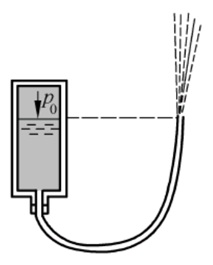
\includegraphics[width=\textwidth]{asset/ch2/T20.png}
    \end{minipage}
\end{example}

\chapter{质点动力学（下）}
\setcounter{example_counter}{1}

\section{动量守恒}

\vspace{-0.3em}

\subsection{动量定理}

\vspace{-0.3em}

\subsubsection{质点的动量定理}

\vspace{-0.3em}

质点的动量$\vec{p}=m\vec{v}$，力$\vec{F}$对质点的冲量为$\vec{I}=\displaystyle\int_{t_1}^{t_2}\vec{F}dt$. 特别地，恒力的冲量$\vec{I}=\vec{F}\Delta t$.

质点所受合外力的冲量等于其动量的变化。

\begin{formula}
    $d\vec{I}=\vec{F}dt=d\vec{p},~~\vec{I}=\displaystyle\int_{t_1}^{t_2}\vec{F}dt=\Delta \vec{p}$
\end{formula}

%\note{质点的动量定理，其实就是牛顿第二定律的变形。}

\subsubsection{质点系的动量定理}

对于多个质点组成的系统，合外力的冲量等于动量的变化，与内力无关。

\begin{formula}
    $\vec{I}_{\text{外}}=\Delta \vec{P}$
\end{formula}

\begin{example}{质点的动量定理}
    粗糙水平面上放一个质量为$\SI{1}{kg}$的物体，静摩擦因数$\mu_s=0.20$，滑动摩擦因数$\mu=0.16$，现用一水平力推该物体，大小$F=t+1$(SI)，$g=\SI{10}{m/s^2}$. 求：(1) 物体所受合外力与$t$的关系；(2) 第$\SI{2}{s}$末的速度；(3) 前两秒内的位移；(4) $F$在前两秒内做的功。

    \tcblower

    (1)~最大静摩擦力$f_m=\mu_s mg=\SI{2}{N}$，当$F=t+1\leq \SI{2}{N}$，即$t\leq \SI{1}{s}$时，推不动物体，合力为零。

    而当$t>\SI{1}{s}$时，已超过静摩擦力，能推动物体，所受合外力为$F-\mu mg=t+1-1.6=t-0.6$(SI)

    \vspace{0.3em}

    (2)~力$F$在$t~(t>1)$时间前的冲量为$\displaystyle\int_1^t{(t-0.6)dt}=\left.\left(\dfrac{1}{2}t^2-0.6t\right)\right|_1^t=0.5t^2-0.6t+0.1$

    \vspace{0.3em}
    
    利用动量定理，可得$0.5t^2-0.6t+0.1=mv$，求得$v=0.5t^2-0.6t+0.1$，代入$t=2$得$v=\SI{0.9}{m/s}$

    \vspace{0.3em}

    (3)~对$v$进行积分可得位移，$x=\displaystyle\int_1^2{(0.5t^2-0.6t+0.1)dt}=\left.\left(\dfrac{1}{6}t^3-0.3t^2+0.1t\right)\right|_1^2=\dfrac{11}{30}~\unit{m}$

    \vspace{0.3em}

    (4)~利用动能定理，$W-\mu mgx=\dfrac{1}{2}mv^2$，得$W=\dfrac{119}{120}\unit{J}$
    
    \tcbline

    %【补充练习】质量为$m$的小球被轻绳挂在天花板上，做圆锥摆运动，角速度为$\omega$. 求转动一周过程中，重力和绳子的拉力对小球的冲量大小。
    
    \begin{minipage}{0.83\textwidth}
    \setlength{\parskip}{0.5em}
    \linespread{1.3}

    【补充练习】质量为$m$的小球被轻绳挂在天花板上，做圆锥摆运动，角速度为$\omega$. 求转动一周过程中，重力和绳子的拉力对小球的冲量大小。
    \end{minipage}
    \hfill
    \begin{minipage}{0.12\textwidth}
        \vspace{-0.5em}
        \centering 
\includegraphics[width=\textwidth]{asset/ch3/T1.png}
    \end{minipage}
    

\end{example}

\begin{example}{连续体的动量定理}
    水平放置的均匀水管弯曲成$90^\circ$，水流量为$\SI{3}{kg/s}$，流速为$\SI{10}{m/s}$，求水流在转角处对弯管的压力大小。（水的密度$\rho=\SI{1e3}{kg/m^3}$）
    \tcblower

    \begin{minipage}{0.82\textwidth}
    \linespread{1.5}
    \setlength{\parskip}{0.1em}
    设水管横截面积为$S$，选择包含弯折部分在内的一段液体作为研究对象。
    
    在$dt$的时间内，发生变化的部分的水的质量$m=Qdt$
    
    它的初末速度可记为$\vec{v}_1=-v\hat{j},~\vec{v}_2=v\hat{i}$

    根据动量定理，$\vec{F}dt=m(\vec{v}_2-\vec{v}_1)$，代入数据得$\vec{F}=\SI{30}(\hat{i}+\hat{j})$
    
    \end{minipage}
    \hfill
    \begin{minipage}{0.15\textwidth}
        \centering 
\includegraphics[width=\textwidth]{asset/ch3/T2.png}
    \end{minipage}

    \vspace{0.3em}

    这说明水管对水的压力大小为$30\sqrt{2}~\unit{N}$，根据牛顿第三定律，水对水管的压力大小也为此值。

    \tcbline

    \begin{minipage}{0.73\textwidth}
    【补充练习】装煤车以$v=\SI{3}{m/s}$的速率在煤斗下方通过，每秒钟落入车厢的煤是$\Delta m=\SI{500}{kg}$，若要使车厢速率不变，忽略摩擦，要用多大的牵引力拉车厢？
    \end{minipage}
    \hfill
    \begin{minipage}{0.25\textwidth}
        \centering 
\includegraphics[width=\textwidth]{asset/ch3/T4.png}
    \end{minipage}
    
\end{example}

\subsection{动量守恒定律}

\subsubsection{动量守恒的条件}

若质点系所受合外力为零，质点系的总动量不变。质点系的内力对总动量不产生影响。

\begin{formula}
    若$\vec{F}_{\text{外}}=\vec{0}$，则$\vec{P}=\mathrm{const.}$
\end{formula}

\begin{example}{动量守恒定律}

    \begin{minipage}{0.78\textwidth}
    质量为$m_A=\SI{2}{kg},~m_B=\SI{3}{kg}$的长方形物体A、B并排放在光滑桌面上，现有质量为$m=\SI{100}{g}$的子弹以速率$v_0=\SI{800}{m/s}$水平射入物体A，经$\SI{0.01}{s}$进入物体B，最后留在物体B内部。若子弹射入A的过程中，所受摩擦力恒
    \end{minipage}
    \hfill
    \begin{minipage}{0.2\textwidth}
        \centering 
\includegraphics[width=\textwidth]{asset/ch3/T3.png}
    \end{minipage}

    \vspace{0.5em}

    为$\SI{3e3}{N}$，求：(1)~子弹射入A的过程中，A对B的作用力大小；(2)~最后A、B的速度大小。

    \tcbline
    
    \setlength{\parskip}{0.1em}

    (1)~在子弹射入A的过程中，A和B是一起运动的，将A、B视为一个整体，$f=(m_A+m_B)a$

    而采用隔离法，只分析B物体，可得$F_{AB}=ma$，代入数据可得$F_{AB}=\SI{1.8e3}{N}$

    (2)~在子弹射入A的过程中，对A、B构成的系统，$ft=(m_A+m_B)v_A$，得$v_A=\SI{6}{m/s}$

    在子弹射入B之后，A与B脱离，A就保持这个速度，而子弹会和B一起继续加速到$v_B$

    对所有物体构成的系统，在整个过程中动量守恒，$mv_0=m_Av_A+(m_B+m)v_B$，解得$v_B\approx \SI{21.9}{m/s}$

    \tcblower
    \setlength{\parskip}{0.1em}
    【补充练习】判断下列说法是否正确：
    
    (1)~作用力与反作用力的冲量之和一定为零；(2)~系统的内力不改变系统的总动量；
    
    (3)~合外力冲量的方向与系统总动量的变化相同；(4)~恒力作用于质点，则时间越长，质点动量越大。
\end{example}

\subsubsection{碰撞}

在碰撞、爆炸等问题中，因为力的作用时间极短，可近似认为动量守恒。

\begin{example}{碰撞}
    在一次粒子散射实验中，质量为$m$的粒子A撞向质量为$M$的静止粒子B。碰撞后A、B的运动方向与A原运动方向的夹角分别为$60^\circ, 30^\circ$，求A粒子碰撞后与碰撞前的速率之比。

    \tcblower

    \begin{minipage}{0.75\textwidth}
    以A原运动方向为$x$正方向
    
    设A粒子碰撞前速率为$v_0$，碰撞后两粒子速率为$v_A,v_B$

    \vspace{0.5em}
        
    根据$y$方向动量守恒，$0=\dfrac{\sqrt{3}}{2}mv_A+\dfrac{1}{2}Mv_B$，即$Mv_B=\sqrt{3}mv_A$

    \vspace{0.5em}

    根据$x$方向动量守恒，$mv_0=\dfrac{1}{2}mv_A+\dfrac{\sqrt{3}}{2}Mv_B$，代入可解得$\dfrac{v_A}{v_0}=\dfrac{1}{2}$
  
    \end{minipage}
    \hfill
    \begin{minipage}{0.22\textwidth}
        \centering 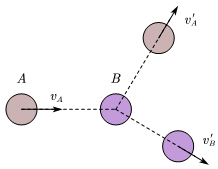
\includegraphics[width=\textwidth]{asset/ch3/T21.png}
    \end{minipage}

    
    
    \tcbline
    【补充练习】
    小球A的质量是B的$4$倍，二者发生碰撞。碰撞前$\vec{v}_A=3\hat{i}+4\hat{j},~\vec{v}_B=2\hat{i}-7\hat{j}$，分别在以下情况下求碰撞后速度: (1) 碰撞后$\vec{v}_B^\prime=7\hat{i}-4\hat{j}$；(2) 碰撞后粘在一起。
\end{example}


\subsubsection{人船模型}

人船模型也可以视为“类碰撞”的情形，在水平方向动量守恒。

%人船模型也可以视为“类碰撞”的情形，水平方向动量守恒，有两种解题思路：
%\begin{itemize}
%    \item 可利用任意时刻的动量为零，得到速度关系，再积分得到位移关系
%    \item 直接利用质心运动定理，质心的水平坐标不变，直接得到位移关系
%\end{itemize}

\begin{example}{人船模型}
    带有1/4圆弧光滑圆槽的大物体质量为$M$，停在光滑的水平面上，滑槽半径为$R$，质量为$m$的小物体自顶点下滑，求小物体滑到底时，大物体在水平面上移动的距离，大物体相对于地面的速度。
    
    \tcblower

    \begin{minipage}{0.7\textwidth}
    (1)~两物体构成的系统在水平方向不受外力，动量守恒
    
    在任意时刻，$0=-MV+mv_x$

    \vspace{0.3em}

    两边同时积分，可得$M\displaystyle\int{Vdt}=m\int{v_xdt}$，即$MS=ms$

    \vspace{0.5em}

    结合几何关系，$S+s=R$，可得$S=\dfrac{m}{M+m}R$

    %\vspace{0.3em}

    %{\fangsong 注：本题也可采用质心运动定理进行求解。
    
    %因为水平方向不受外力，所以质心的横坐标不会变化。

    %\vspace{0.5em}

    %根据$0=\dfrac{-MS+m(R-S)}{M+m}$，也可解得$S=\dfrac{m}{M+m}R$}

    \vspace{0.5em}
    
    (2)~小物体滑到底端时，小物体速度为水平方向
    
    根据动量守恒定律，仍有$0=-MV+mv$

    \vspace{0.5em}

    根据机械能守恒定律，$mgR=\dfrac{1}{2}MV^2+\dfrac{1}{2}mv^2$

    \vspace{0.5em}

    联立两式解得$V=\sqrt{\dfrac{2m^2gR}{M(M+m)}}$
  
    \end{minipage}
    \hfill
    \begin{minipage}{0.27\textwidth}
        \centering 
\includegraphics[width=\textwidth]{asset/ch3/T5.png}
    \end{minipage}

    \tcbline
    
    \begin{minipage}{0.78\textwidth}
    【补充练习】质量为$m$的小物体从质量为$M$、倾角为$\theta$、长为$L$的斜面顶端静止滑落，不计摩擦，求小物体滑落到斜面底端时，斜面的位移和速度。
    \end{minipage}
    \hfill
    \begin{minipage}{0.2\textwidth}
        \centering 
\includegraphics[width=\textwidth]{asset/ch3/T6.png}
    \end{minipage}
       
\end{example}

\section{角动量守恒}

\subsection{角动量定理}

\subsubsection{力矩}

对固定点O而言，若质点的位置矢量为$\vec{r}$，则力$\vec{F}$的力矩定义为$\vec{M}=\vec{r}\times \vec{F}$

力矩的大小其实就是杠杆原理中的力乘以力臂，方向可简化区分顺时针/逆时针转动。

\note{如果力过固定点O，则力臂为零，力矩就为零，因为对于转动无作用。}

\subsubsection{角动量}

对固定点O而言，质点的角动量定义为$\vec{L}=\vec{r}\times \vec{p}=\vec{r}\times (m\vec{v})$

角动量的大小与力矩计算方法类似，等于动量乘以动量臂，方向也可简化区分顺时针/逆时针转动。

\note{特别地，对于圆周运动而言，对圆心的动量臂等于半径$R$，所以角动量的大小就等于$mvR$。}

\begin{figure}[htb]
    \centering
    
\includegraphics[width=0.45\linewidth]{asset/ch3/T7.png} 
\includegraphics[width=0.45\linewidth]{asset/ch3/T8.png}
\end{figure}

\begin{formula}
    $\text{力矩}M\text{的大小}=\text{力}F\times \text{力臂}$，$\text{角动量}L\text{的大小}=\text{动量}mv\times \text{动量臂}$
\end{formula}

\subsubsection{角动量定理}

对一个固定点O，合外力矩等于角动量的变化率。
\begin{formula}
    $\vec{M}=\dfrac{d\vec{L}}{dt},~~\displaystyle\int_0^t{\vec{M}dt}=\Delta \vec{L}$
\end{formula}

\subsection{角动量守恒定律}

对一个固定点O，若合外力矩为零，则系统的角动量守恒。

\warn{角动量守恒必须选定固定点O，对不同的点，角动量守恒的判断结果不同。}

\begin{formula}
    若$\vec{M}=\vec{0}$，则$\vec{L}=\mathrm{const.}$
\end{formula}

\note{如果系统不受外力，或外力过所选择的固定点，则合外力矩为零，就能满足角动量守恒的要求。例如，行星运动过程中，相对于中心天体的角动量守恒。}

\note{但是系统所受合外力是零，并不能说明合力矩也是零，因为两个力可能不共线，角动量不一定守恒。}

\begin{example}{角动量守恒定律}
    人造卫星绕地球沿椭圆轨道运动，地球半径为$R$，卫星到地面的最近、最远距离为$h_1,h_2$，(1)~若已知近地点速率为$v_1$，求远地点速率；(2)~若已知地球质量为$M$，求近地点和远地点速率。
    \tcblower

    (1)~根据角动量守恒定律，$mv_1(R+h_1)=mv_2(R+h_2)$，可得$v_2=v_1\dfrac{R+h_1}{R+h_2}$

    \vspace{0.5em}

    (2)~根据机械能守恒定律，$\dfrac{1}{2}mv_1^2+\left(-\dfrac{GMm}{R+h_1}\right)=\dfrac{1}{2}mv_2^2+\left(-\dfrac{GMm}{R+h_2}\right)$

    \vspace{0.5em}

    {\fangsong 注：此处不能用重力势能，而要用万有引力势能，注意万有引力势能的表达式自带负号。}

    结合角动量守恒定律$mv_1(R+h_1)=mv_2(R+h_2)$

    \vspace{0.5em}
    
    可联立解得$v_1=\sqrt{\dfrac{2GM(R+h_2)}{(R+h_1)(2R+h_1+h_2)}},~v_2=\sqrt{\dfrac{2GM(R+h_1)}{(R+h_2)(2R+h_1+h_2)}}$
   
    \tcbline

    \begin{minipage}{0.73\textwidth}
    【补充练习】质量为$m$的小球系于轻绳一端，另一端穿过桌面上的小孔并用手拉住。先使小球做半径为$r_0$的圆周运动，角速度为$\omega_0$；若拉动轻绳，使运动半径变为$r$。求：此时的角速度和拉力，拉力在这一过程中所做的功。
    \end{minipage}
    \hfill
    \begin{minipage}{0.25\textwidth}
        \centering 
\includegraphics[width=\textwidth]{asset/ch3/T9.png}
    \end{minipage}

\end{example}

\subsection{三大守恒的对比}

\begin{table}[htb]
    \centering
    \begin{tabular}{|c|c|c|}
        \hline
        守恒定律 & 条件 & 是否与内力有关\\
         \hline
        动量守恒 & 合外力为零 & 无关 \\
         \hline
        角动量守恒 & 合外力矩为零 & 无关 \\
         \hline
        机械能守恒 & 只有保守内力做功 & 有关 \\
         \hline
    \end{tabular}
\end{table}

\note{三大守恒分别对应了三种不同的对称性，彼此是相互独立的，任何一个物理量守恒，都不能直接推出其他的守恒结论。但单个质点的动量守恒，则角动量一定守恒。}

\begin{example}{三大守恒的对比}
    \setlength{\parskip}{0.1em}
    判断在以下情境中，动量、机械能、对圆心的角动量是否守恒。

    (1)~竖直平面内由绳牵引的圆周运动；(2)~竖直平面内由杆控制的匀速圆周运动

    \tcblower

    \setlength{\parskip}{0.1em}

    判断是否守恒可以从条件上判断，也可以从结果上判断。

    (1)~只有重力做功，机械能守恒；速度的大小和方向时刻变化，所以动量、角动量不守恒。

    (2)~速度大小不变，半径不变，所以角动量守恒；速度方向改变，所以动量不守恒；动能不变，势能改变，机械能不守恒。
    
    \tcbline

    \setlength{\parskip}{0.1em}
    
    【补充练习】一质点在几个外力同时作用下运动时，判断下列叙述是否正确。
    
    (1)~若质点的动量改变，动能一定改变；(2)~若动量守恒，则机械能守恒；

    (3)~若动量守恒，则对任意点的角动量守恒；(4)~若外力做功为零，外力的冲量一定为零；
    
    (5)~若机械能守恒，则动量守恒；(6)~若对一点的角动量守恒，则对其他任意点的角动量也守恒

\end{example}

\section{拓展内容}

\subsection{变质量系统的动量守恒}

如果系统质量发生变化，则不能贸然使用牛顿第二定律，动量的变化需要同时考虑质量和速度的变化。

使用数学上的全微分，可知

\begin{formula}
    $d\vec{p}=m\cdot d\vec{v}+\vec{v}\cdot dm$
\end{formula}

\begin{example}{变质量系统的动量守恒*}
    (1) 质量为$M$的火箭以速度$v$运动，以相对速率$u$向后扔出一个质量为$m$的球，求火箭的速度。

    (2) 质量为$M$的火箭以速度$v$运动，以相对速率$u$持续向后喷出气体，求质量减小$m$时的速度。

    \tcblower
    
    (1)~飞船的初动量为$Mv$，且动量守恒，$Mv=(M-m)v^\prime+m(v^\prime-u)$，解得$v^\prime=v+\dfrac{m}{M}u$

    (2)~在$dt$时间内，假设喷出气体质量为$dm$，速度增加$dv$
    
    则飞船的动量变为$(M-dm)(v+dv)$，而喷出气体的动量为$dm(v+dv-u)$（注意速度方向）

    \vspace{0.25em}

    根据动量守恒定律，$Mv=(M-dm)(v+dv)+(v+dv-u)dm$，整理得$dv=\dfrac{u}{M}dm$

    \vspace{0.5em}

    结合$dm=-dM$，两边积分得$\displaystyle\int{dv}=-\int\dfrac{u}{M}dM$，即$v^\prime-v=u[\ln{M}-\ln{(M-m)}]$

    \vspace{0.5em}

    整理得$v^\prime=v+u\ln{\dfrac{M}{M-m}}$

    \tcbline
    【补充练习】均匀竖直链条长度为$l$，质量为$m$，下端刚触地，求自由下落$h$时对地面的作用力。
\end{example}

\chapter{刚体定轴转动}
\setcounter{example_counter}{1}

\section{刚体转动的描述}

\subsection{刚体}

\textbf{刚体}是受力时形状和大小不发生改变的物体，是一种理想模型。

\subsection{刚体转动的描述}

对于刚体的定轴转动，我们只关心其转过的角度，因此可用角位移$\theta$、角速度$\omega$、角加速度$\alpha$描述，它们的关系与圆周运动的质点相同。

\begin{figure}[htb]
    \centering
    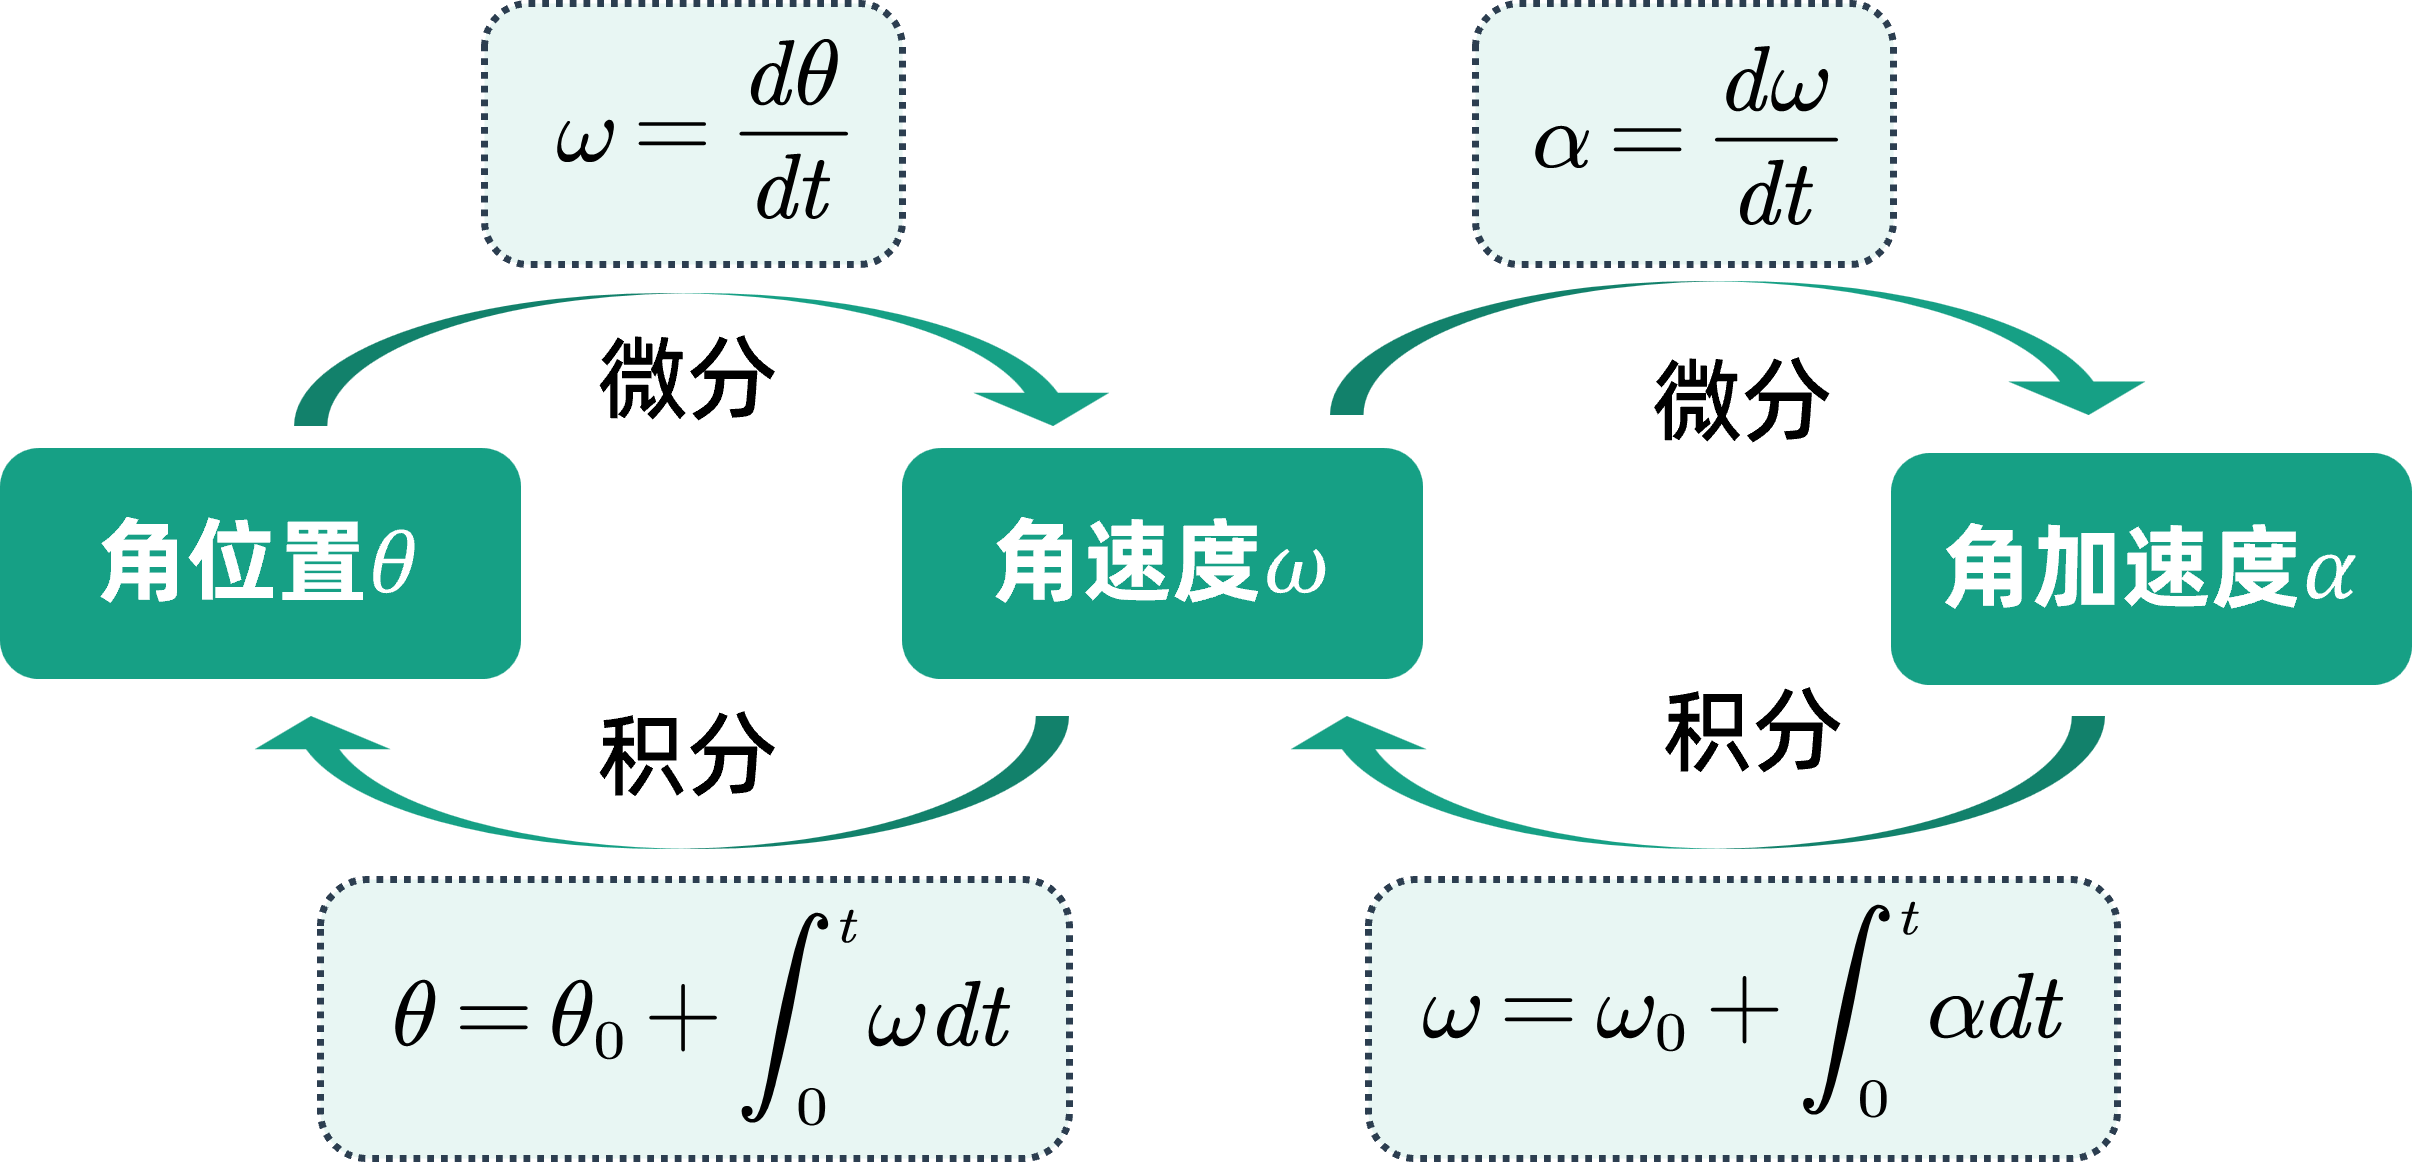
\includegraphics[width=0.6\linewidth]{asset/ch1/T8.png}
\end{figure}

\begin{formula}
    $\omega=\dfrac{d\theta}{dt},~\alpha=\dfrac{d\omega}{dt},~\theta=\theta_0+\displaystyle\int_0^t{\omega dt},~\omega=\omega_0+\displaystyle\int_0^t{\alpha dt}$
\end{formula}

\note{转动的角位移$\theta$、角速度$\omega$、角加速度$\alpha$的关系，与直线运动的位移$x$、速度$v$、加速度$a$的关系完全相同。}

\begin{example}{转动的描述}
    飞轮从$\SI{5}{rad/s}$开始均匀减速，在$\SI{20}{s}$后，角速度减为原来的$80\%$。求前$\SI{150}{s}$内转过的角度。
    \tcblower
    仿照匀变速直线运动的公式，把线量替换成角量，注意刹车陷阱。

    根据$\omega_1=\omega_0+\alpha t_1$，得角加速度$\alpha=\SI{-0.05}{rad/s^2}$，飞轮停下来的时间$t$满足$0=\omega_0+\alpha t_1$
    
    求得$t=\SI{100}{s}$，说明飞轮在$t=\SI{100}{s}$时就已经停下来，$\SI{150}{s}$是干扰信息。

    飞轮转过的角度$\theta$满足$0-\omega_0^2=2\alpha \theta$，得$\theta=\SI{250}{rad}$
    \tcbline
    【补充练习】汽车发动机的主轴，在$\SI{7.0}{s}$的时间内，从$\SI{200}{r/min}$均匀增加到$\SI{3000}{r/min}$. 求：角加速度、这段时间内转过的圈数。
\end{example}

\section{刚体的转动定律}

\subsection{转动惯量}

\subsubsection{转动惯量的定义}

质点惯性的度量是质量，而刚体惯性的度量是\textbf{转动惯量}$J$，计算方法如下。

\begin{formula}
    $J=\sum{m_ir_i^2}$
\end{formula}

\note{刚体的转动惯量与质量、质量的分布、转轴的位置有关。}

\note{质量越大、离转轴越远，转动惯量就越大，在转轴上的部分对转动惯量没有贡献。}

\subsubsection{转动惯量的计算}

在计算组合体的转动惯量时，可拆成多个部分计算后再相加：

\begin{itemize}
    \item 对于孤立的质点，对转轴的转动惯量就是$J=MR^2$
    \item 对于连续型的物体，则需要切成小段之后积分求解，$J=\displaystyle\int{r^2dm}$
\end{itemize}

\subsubsection{典型物体的转动惯量}

以下常见均匀物体的转动惯量需要记忆，可在考试中直接使用。

\newcolumntype{C}[1]{>{\centering\arraybackslash}m{#1}}
\begin{table}[htb]
    \centering
    \begin{tabular}{|C{3cm}|C{3cm}|C{3cm}|C{2.5cm}|}
        \hline
        刚体形状 & 图示 & 转轴 & 转动惯量\\
        \hline
        \rule[-12pt]{0pt}{0pt} 细杆 & 
\includegraphics[width=0.12\textwidth]{asset/ch4/T7.png} & 通过一端垂直于杆 &  $J=\dfrac{1}{3}ml^2$\\
        \hline
        细杆 & 
\includegraphics[width=0.12\textwidth]{asset/ch4/T6.png} & 通过中点垂直于杆 & $J=\dfrac{1}{12}ml^2$\\
        \hline
        圆环/空心圆筒 & 
\includegraphics[width=0.08\textwidth]{asset/ch4/T4.png} & 通过圆心垂直于环 & $J=mR^2$\\
        \hline
        圆盘/空心圆柱 & 
\includegraphics[width=0.08\textwidth]{asset/ch4/T5.png} & 通过圆心垂直于盘 & $J=\dfrac{1}{2}mR^2$\\
        \hline
        空心球壳 & 
\includegraphics[width=0.05\textwidth]{asset/ch4/T8.png} & 直径 & $J=\dfrac{2}{3}mR^2$\\
        \hline
        实心球 & 
\includegraphics[width=0.05\textwidth]{asset/ch4/T9.png} & 直径 & $J=\dfrac{2}{5}mR^2$\\
        \hline
    \end{tabular}
\end{table}

\begin{example}{转动惯量的计算}
    长度为$l$、质量为$m$的均匀细杆，一端固定在天花板上，另一端和中点处各固定一个质量为$m$的小球（小球可视为质点）。求该整体对转轴的转动惯量。
    \tcblower

    \begin{minipage}{0.83\textwidth}

    这是一个组合体，可以拆成两个小球和一根细杆分别计算。

    \vspace{0.3em}
    
    两个小球到转轴的距离分别为$\dfrac{l}{2},~l$，它们转动惯量合计是$m\left(\dfrac{l}{2}\right)^2+ml^2=\dfrac{5}{4}ml^2$

    \vspace{0.5em}

    均匀细杆可切分为长度为$dx$的许多小段，每段质量为$\dfrac{mdx}{l}$。

    \vspace{0.5em}
    
    到转轴距离为$x$的小段，转动惯量是$\dfrac{mdx}{l}x^2$

    \vspace{0.5em}

    所以细杆的转动惯量为$\displaystyle \int_0^l{\dfrac{mdx}{l}x^2}=\left.\dfrac{mx^3}{3l}\right|_0^l=\dfrac{1}{3}ml^2$

    \vspace{0.5em}
    
    因此整个整体的转动惯量为$J=\dfrac{5}{4}ml^2+\dfrac{1}{3}ml^2=\dfrac{19}{12}ml^2$
    \end{minipage}
    \hfill
    \begin{minipage}{0.15\textwidth}
        \centering 
\includegraphics[width=\textwidth]{asset/ch4/T1.png}
    \end{minipage}

    \tcbline
    
    \begin{minipage}{0.78\textwidth}

    【补充练习】一个长为$2L$、质量为$2m$的均匀铁丝在中点处弯折成$120^\circ$，如图所示，AO边与$x$轴重合。求该铁丝AOB对于$x$轴的转动惯量。
    \end{minipage}
    \hfill
    \begin{minipage}{0.2\textwidth}
        \centering 
\includegraphics[width=\textwidth]{asset/ch4/T2.png}
    \end{minipage}
\end{example}

\subsection{转动定律}

对于某一固定轴，刚体所受合外力矩$M$，等于转动惯量$J$与角加速度$\alpha$的乘积。
\begin{formula}
    $F=ma~~~\rightarrow~~~M=J\alpha$
\end{formula}

\note{上述公式就是把牛顿第二定律中的线量全部换为角量，该公式仅针对刚体定轴转动成立。}

\note{力矩的大小等于力乘以力臂，需要区分力矩驱动顺时针还是逆时针转动。}

\begin{example}{转动定律（单物体）}
    长度为$l$、质量为$m$的细杆，一端固定在天花板上，另一端与质量为$m$的小球相连（小球可视为质点），从水平位置向下摆动。求摆动$\theta$角时，摆动的角加速度大小。
    \tcbline

    \begin{minipage}{0.78\textwidth}
    细杆和小球构成的整体可看做一个刚体，转动惯量$J=\dfrac{1}{3}ml^2+ml^2=\dfrac{4}{3}ml^2$

    \vspace{0.3em}

    刚体的受力包括重力和转轴给的力，但转轴给的力过转轴，对转动没有作用。

    \vspace{0.3em}

    杆的重力可视为作用于重心，力臂是$\dfrac{l}{2}\cos{\theta}$，而小球的重力的力臂是$l\cos{\theta}$

    \vspace{0.5em}

    因此刚体受力对转轴的力矩为$M=mg\dfrac{l}{2}\cos{\theta}+mgl\cos{\theta}=\dfrac{3}{2}mgl\cos{\theta}$

    \vspace{0.5em}

    根据转动定律，$M=J\alpha$，可得角加速度$\alpha=\dfrac{9g\cos{\theta}}{8l}$
    \end{minipage}
    \hfill
    \begin{minipage}{0.2\textwidth}
        \centering 
\includegraphics[width=\textwidth]{asset/ch4/T11.png}
    \end{minipage}
    
    \tcblower
    
    \begin{minipage}{0.83\textwidth}
    【补充练习】如图所示，半径为$R$、质量为$M$的均匀圆盘可绕过圆心的固定轴任意转动。大小相等、方向相反的力$F$，分别作用于边缘和半径中点，不计所有摩擦。(1)~求圆盘转动的角加速度大小；(2)~判断圆盘现在是加速还是减速；
    
    (3)~当圆盘的角速度从$\omega_0$变为$\omega$时，求经过的时间$t$和转过的角度$\theta$.
    \end{minipage}
    \hfill
    \begin{minipage}{0.15\textwidth}
        \centering 
\includegraphics[width=\textwidth]{asset/ch4/T12.png}
    \end{minipage}
\end{example}

\begin{example}{转动定律（多物体）}

    \vspace{-0.5em}
    
    \begin{minipage}{0.73\textwidth}
    如图所示，定滑轮可看作半径为$R$、质量为$3m$的匀质圆盘，绳在圆盘处无滑动，忽略其他摩擦，由静止释放。已知物体质量分别为$m,2m$，求：(1)~两侧绳拉力和物体运动的加速度；(2)~物体下落$h$时圆盘的角速度。
    
    \end{minipage}
    \hfill
    \begin{minipage}{0.25\textwidth}
        \centering 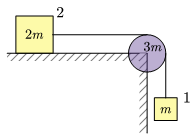
\includegraphics[width=\textwidth]{asset/ch4/T13.png}
    \end{minipage}

    \vspace{-0.5em}
    
    \tcblower
    
    (1)~在本题中，圆盘和两个物体不能视为一个刚体，需要用隔离法分别分析。

    两个物体运动的加速度相同，设为$a$，但要注意两侧绳拉力是不同的。
    
    由牛顿第二定律，$mg-T_1=ma,~T_2=2ma$，根据线量与角量的关系，$a=\alpha R$

    \vspace{0.3em}
    
    对于圆盘，转动惯量为$J=\dfrac{1}{2}3mR^2$，两个力的力臂都是$R$，但方向相反

    \vspace{0.3em}
    
    所以合外力矩$M=(T_1-T_2)R$，代入转动定律得$(T_1-T_2)R=\dfrac{1}{2}\cdot 3mR^2\cdot \alpha$

    \vspace{0.3em}

    联立以上各式解得$a=\dfrac{2}{9}g,~T_1=\dfrac{7}{9}mg,~T_2=\dfrac{4}{9}mg$

    \vspace{0.3em}

    (2)~利用匀变速直线运动规律，$v^2=2ah$. 根据线量和角量的关系，$v=\omega R$，解得$\omega=\dfrac{2\sqrt{2gh}}{3R}$

    \tcbline

    \vspace{-0.5em}
    
    \begin{minipage}{0.85\textwidth}
    【补充练习】半径分别为$R,2R$、质量分别为$m,4m$的均匀圆盘，同轴地粘在一起，可绕过盘心且垂直盘面的水平光滑轴任意转动。两盘边缘都绕有轻绳，下端分别挂有质量均为$m$的物体A、B。求物体A、B运动的加速度。
    \end{minipage}
    \hfill
    \begin{minipage}{0.12\textwidth}
        \centering 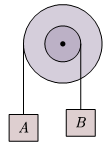
\includegraphics[width=\textwidth]{asset/ch4/T14.png}
    \end{minipage}
    
\end{example}

\section{转动中的功与能}

\subsection{动能定理}

%\subsubsection{力矩做功}

力矩$M$所做的功，就是力矩在角度上的积累。
\begin{formula}
    $W=\displaystyle\int{Fdx}~~~\rightarrow~~~W=\displaystyle\int{Md\theta}$
\end{formula}

%\subsubsection{刚体的转动动能}

绕定轴转动的刚体转动动能可表示为

\begin{formula}
    $E_k=\dfrac{1}{2}mv^2~~~\rightarrow~~~E_k=\dfrac{1}{2}J\omega^2$
\end{formula}

%\subsubsection{动能定理}

合外力矩对定轴转动刚体所做的功，等于转动动能的增量。

\begin{formula}
    $W=\displaystyle\int{Md\theta}=\Delta E_k=\dfrac{1}{2}J\omega_2^2-\dfrac{1}{2}J\omega_1^2$
\end{formula}

%\note{仿照$E_k=\dfrac{1}{2}mv^2$，把$m$替换成$J$，把$v$替换成$\omega$即可。}

\subsection{机械能守恒定律}

\subsubsection{刚体的重力势能}

只要刚体不太大，刚体的重力势能，只需将高度代入质心所在的高度即可。
\begin{formula}
    $E_p=mgh~~~\rightarrow~~~E_p=mgh_C$
\end{formula}

%\note{仿照力的做功，把$F$替换成$M$，把$x$替换成$\theta$即可。}

\subsubsection{守恒定律}

对于包括刚体在内的系统，动能定理、功能原理和机械能守恒定律仍然成立。

如果只有保守内力做功，则系统机械能守恒。

%\note{刚体本身就是一个质点系，所以质点系的动能定理、机械能守恒定律都仍然成立。}

\begin{example}{刚体与机械能守恒}
    \begin{minipage}{0.8\textwidth}
    如图所示，滑轮可视为均匀圆盘，质量为$M$，半径为$R$。在初始状态下，劲度系数为$k$的轻弹簧处于原长，质量为$m$的物体静止于倾角为$\theta$的光滑固定斜面上。求：(1) 重物沿斜面下滑$L$距离后的速度大小；(2) 重物下滑的最远距离。
    \end{minipage}
    \hfill
    \begin{minipage}{0.18\textwidth}
        \centering 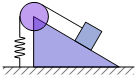
\includegraphics[width=\textwidth]{asset/ch4/T16.png}
    \end{minipage}
    \tcblower

    (1)~在此过程中，只有重力和弹簧弹力做功，系统的机械能守恒。
    
    重力势能转化为弹簧的弹性势能和滑轮与重物的动能，$mgL\sin{\theta}=\dfrac{1}{2}kL^2+\dfrac{1}{2}mv^2+\dfrac{1}{2}J\omega^2$

    \vspace{0.5em}

    均匀圆盘的转动惯量$J=\dfrac{1}{2}MR^2$，根据线量与角量的关系，$v=\omega R$

    \vspace{0.5em}

    联立以上各式解得$v=\sqrt{\dfrac{4mgL\sin\theta-2kL^2}{M+2m}}$

    \vspace{0.5em}
    
    (2)~重物下滑最远距离时，速度为零，重力势能完全转化为弹簧的弹性势能。
    
    \vspace{0.5em}

    由$mgL\sin{\theta}=\dfrac{1}{2}kL^2$，得$L=\dfrac{2mg\sin{\theta}}{k}$
    
    \tcbline

    \vspace{-1em}

    \begin{minipage}{0.8\textwidth}
    【补充练习】长为$L$、质量为$m$的均匀细杆可绕光滑固定轴O在竖直面内旋转，细杆由静止自由下摆，求棒转过$\theta$角时的角速度和角加速度。
    \end{minipage}
    \hfill
    \begin{minipage}{0.18\textwidth}
        
        \centering 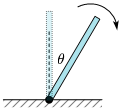
\includegraphics[width=\textwidth]{asset/ch4/T15.png}
    \end{minipage}

    \vspace{-0.5em}
\end{example}

\section{角动量守恒}

\subsection{刚体的角动量}

在质点动力学中，我们已经学习过质点对轴的角动量，等于动量乘以动量臂。

刚体对轴的角动量$L$，等于转动惯量乘以角速度。

\begin{formula}
    $p=mv~~~\rightarrow~~~L=J\omega$
\end{formula}

对于刚体和质点组成的系统，角动量就是系统内所有研究对象的角动量之和。

\subsection{角动量定理}

力矩在时间上的积累称为角冲量或冲量矩$H$，刚体所受角冲量等于角动量的变化$\Delta L$。

\begin{formula}
    $I=\displaystyle \int{Fdt}=\Delta p=p_2-p_1~~~\rightarrow~~~H=\displaystyle \int{Mdt}=\Delta L=L_2-L_1=J\omega_2-J\omega_1$
\end{formula}

\note{动量定理说明冲量等于动量的变化，而角动量定理说明角冲量等于角动量的变化。}

%若考虑刚体和质点组成的系统，则合外力矩的角冲量等于系统角动量的变化，内力矩不产生影响。

\subsection{角动量守恒定律}

对刚体和质点组成的系统，若合外力矩为零，则角动量守恒。

\begin{formula}
    若$M_{\text{外}}=0$，则$L$不变。
\end{formula}

\note{若合外力为零，则动量守恒；若合外力矩为零，则角动量守恒。}

一种常见的情况是，若刚体可绕转轴自由旋转，所受外力全部过转轴，则角动量守恒。

\begin{example}{刚体与角动量守恒}
    \begin{minipage}{0.82\textwidth}
    有半径为$R$、质量为$M$的均匀水平转台，可绕过圆心的转轴自由旋转，中间有一个质量为$m$的人，初始角速度为$\omega_0$，从上向下看为顺时针旋转。
    
    (1)~若人走到转台边缘，并于转台相对静止，求此时的角速度。

    (2)~若人相对圆盘以恒定速率$v$逆时针沿边缘运动，求圆盘的角速度。
    
    \end{minipage}
    \hfill
    \begin{minipage}{0.15\textwidth}
        \centering 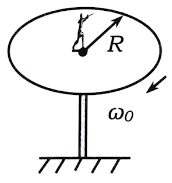
\includegraphics[width=\textwidth]{asset/ch4/T17.png}
    \end{minipage}

    \tcblower

    转台可绕转轴自由旋转，若以人和圆盘组成的系统为研究对象，人与转台之间的力是内力，则所受外力全部过转轴，系统角动量守恒。
    
    (1)~在初状态，人位于圆心，对转动惯量和角动量无贡献。
    
    因此初角动量只需考虑圆盘的贡献，转动惯量$J_1=\dfrac{1}{2}MR^2$，角动量$L_1=J_1\omega_0$

    \vspace{0.5em}
    
    而在末状态，人位于边缘且相对圆盘静止，需要考虑其对转动惯量的贡献。

    \vspace{0.3em}
    
    将人与圆盘视为一个整体，这个整体的转动惯量$J_2=\dfrac{1}{2}MR^2+mR^2$，角动量$L_2=J_2\omega$

    \vspace{0.5em}
    
    根据角动量守恒定律，$L_1=L_2$，解得$\omega=\dfrac{M}{M+2m}\omega_0$

    \vspace{0.5em}

    (2)~在末状态，人和圆盘需要分别计算角动量，系统的角动量是二者之和。

    \vspace{0.3em}
    
    圆盘的转动惯量仍为$J_1=\dfrac{1}{2}MR^2$，角动量为$\dfrac{1}{2}MR^2\omega$

    \vspace{0.5em}

    若以顺时针为正方向，则人相对于大地的速率是$\omega R-v$，因此角动量为$m(\omega R-v)R$

    （回忆第2章质点角动量的知识，匀速圆周运动的质点，其角动量大小为$mvR$）

    \vspace{0.5em}

    根据角动量守恒定律，$L_1=\dfrac{1}{2}MR^2\omega+m(\omega R-v)R$，解得$\omega=\dfrac{MR\omega_0+2mv}{(M+2m)R}$
    
    \tcbline
    \begin{minipage}{0.8\textwidth}
    
    【补充练习】判断下列说法是否正确：(1)~作用力与反作用力的力矩之和为零；(2)~两个等大反向的力作用在刚体上，刚体的角动量不变；(3)~内力矩不改变系统的角动量；(4)~两个相同质量的子弹同时相向射入并留在旋转的盘子内部（如图所示），盘子转动的角速度不变。
    
    \end{minipage}
    \hfill
    \begin{minipage}{0.18\textwidth}
        \centering 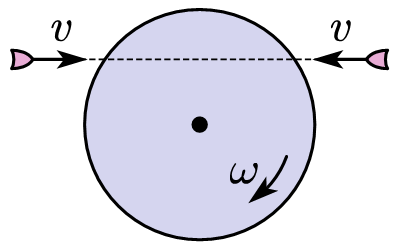
\includegraphics[width=\textwidth]{asset/ch4/T18.png}
    \end{minipage}
    
\end{example}

\subsection{碰撞}

质点的碰撞通常考虑动量守恒，而刚体转动中的碰撞通常考虑角动量守恒。

\note{这是因为在碰撞瞬间，虽然时间极短，但转轴产生的冲击力也很大，不可忽略，所以外力不为零，动量一般不守恒。但是转轴产生的冲击力通过转轴，合外力矩为零，因此碰撞物体构成的系统，角动量守恒。}

\begin{example}{刚体转动与碰撞}
    \begin{minipage}{0.8\textwidth}
    均匀细杆长为$L$，质量为$6m$，被光滑轴固定在天花板上。一个质量为$m$的子弹以速度$v$射入细杆自由端，并留在细杆内。(1)~研究细杆和子弹组成的系统，判断碰撞前后，机械能、动量、对转轴的角动量是否守恒。(2)~求碰撞后瞬间细杆的角速度；(3)~求细杆最大摆角的余弦值。
    
    \end{minipage}
    \hfill
    \begin{minipage}{0.18\textwidth}
        \centering 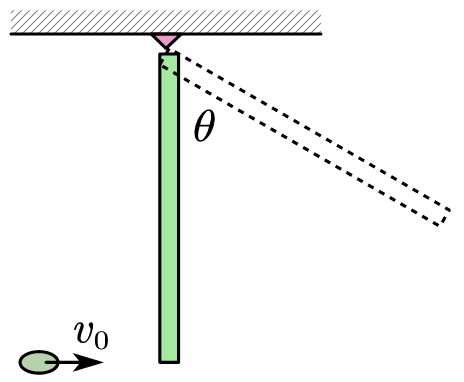
\includegraphics[width=\textwidth]{asset/ch4/T19.png}
    \end{minipage}

    \tcblower
    \setlength{\parskip}{0.1em}

    (1)~由于子弹留在细杆中，相当于完全非弹性碰撞，能量损失最大，机械能不守恒。

    在碰撞瞬间，虽然时间极短，但是转轴处产生的冲击力不可忽略，合外力不为零，动量不守恒。

    但是转轴处产生的冲击力通过转轴，合外力矩为零，所以对转轴的角动量守恒。

    (2)~碰撞前只有子弹在运动，系统角动量$L_1=mvL$

    \vspace{0.3em}

    碰撞后二者结合在一起运动，系统转动惯量$J=\dfrac{1}{3}\cdot 6mL^2+mL^2$，角动量$L_2=J\omega$

    \vspace{0.5em}

    碰撞前后角动量守恒，由$L_1=L_2$解得碰撞后瞬间角速度$\omega=\dfrac{v}{3L}$

    \vspace{0.5em}

    (3)~在碰撞后摆动的过程中，只有重力做功，系统机械能守恒，系统的重力势能可以分别计算。

    \vspace{0.5em}

    由$\dfrac{1}{2}J\omega^2=6mg\dfrac{L}{2}(1-\cos\theta)+mgL(1-\cos\theta)$，求得$\cos\theta=1-\dfrac{3v^2}{8gL}$
    
    \tcbline
    

    \begin{minipage}{0.8\textwidth}
    【补充练习】质量为$m$的黏土块，以水平速度$v$撞在竖直平面的静止圆盘顶端，并粘在一起。圆盘半径为$R$，质量为$2m$，圆盘轴光滑。求：(1)~碰撞后瞬间圆盘的角速度；(2)~圆盘转过$90^\circ$时的角速度。
    
    \end{minipage}
    \hfill
    \begin{minipage}{0.18\textwidth}
        \centering 
\includegraphics[width=\textwidth]{asset/ch4/T20.png}
    \end{minipage}
\end{example}

\subsection{质点与刚体的对比}

\begin{center}
    \begin{tabular}{|c|c|c|}
        \hline
         & 质点 & 刚体 \\
        \hline
        运动的描述 & 线量$x,v,a$ & 角量$\theta, \omega, \alpha$ \\
        \hline
        惯性的度量 & 质量$m$ & 转动惯量$J$ \\
        \hline
        运动定律 & $F=ma$ & $M=J\alpha$ \\
        \hline
        \rule{0pt}{18pt}\rule[-12pt]{0pt}{0pt} 动能 & $E_k=\dfrac{1}{2}mv^2$ & $E_k=\dfrac{1}{2}J\omega^2$ \\
        \hline
        \rule{0pt}{18pt}\rule[-12pt]{0pt}{0pt} 动能定理 & $\displaystyle\int{Fdx}=\Delta E_k$ & $\displaystyle\int{Md\theta}=\Delta E_k$ \\
        \hline
        重力势能 & $E_p=mgh$ & $E_p=mgh_C$ \\
        \hline
        机械能守恒条件 & 只有保守内力做功 & 只有保守内力做功 \\
        \hline
        动量/角动量 & $p=mv$ & $L=J\omega$ \\
        \hline
        \rule{0pt}{18pt}\rule[-12pt]{0pt}{0pt} 动量/角动量定理 & $\displaystyle\int{Fdt}=\Delta p$ & $\displaystyle\int{Mdt}=\Delta L$ \\
        \hline
        动量/角动量守恒条件 & 合外力为零 & 合外力矩为零 \\
        \hline
    \end{tabular}
\end{center}


\section{拓展内容}

\subsection{计算转动惯量的其他方法}

\subsubsection{平行轴定理}

刚体的转动惯量与转轴的选取有关，如果需要平移转轴，可以使用平行轴定理。

若已知转轴过质心的转动惯量$J_C$，将转轴平行移动距离$d$后，转动惯量$J$的公式为
\begin{formula}
    $J=J_C+md^2$
\end{formula}

\warn{注意平行轴定理的基准一定是过质心的转动惯量。}

\subsubsection{正交轴定理}

对于$xy$平面上的薄平板刚体，它对于三个坐标轴的转动惯量满足

\begin{formula}
    $J_z=J_x+J_y$
\end{formula}

例如，以一条直径为轴，圆环的转动惯量$J=\dfrac{1}{2}MR^2$，圆盘的转动惯量$J=\dfrac{1}{4}MR^2$.


\begin{center}
    
\includegraphics[width=0.35\linewidth]{asset/ch4/T21.png}
\end{center}
    
\begin{example}{平行轴定理*}
    如图所示，长为$L$、质量为$m_1$的均匀细杆，一端与转轴相连，另一端连接半径为$r$、质量为$m_2$的均匀圆盘。求整个物体相对于转轴的转动惯量。
    \tcbline

    \begin{minipage}{0.83\textwidth}

    对于细杆而言，转轴位于一端，转动惯量为$\dfrac{1}{3}m_1L^2$

    \vspace{0.3em}

    对于圆盘而言，转轴转轴到圆心的距离是$L+r$，需要使用平行轴定理。

    \vspace{0.3em}
    
    对于过圆心的转轴，转动惯量为$J_0=\dfrac{1}{2}m_2r^2$
    
    \vspace{0.5em}

    利用平行轴定理可知转动惯量变为$\dfrac{1}{2}m_2r^2+m_2(L+r)^2$

    \vspace{0.5em}

    因此整个物体的转动惯量为$J=\dfrac{1}{3}m_1L^2+\dfrac{1}{2}m_2r^2+m_2(L+r)^2$
    \end{minipage}
    \hfill
    \begin{minipage}{0.15\textwidth}
        \centering 
\includegraphics[width=\textwidth]{asset/ch4/T3.png}
    \end{minipage}
    
    \tcblower

    \begin{minipage}{0.69\textwidth}
    【补充练习】三根长为$L$、质量为$m$的均匀细杆焊接成一个等边三角形，转轴垂直于这个三角形所在平面，且过其中一个顶点。求这个物体相对于该转轴的转动惯量。
    \end{minipage}
    \hfill
    \begin{minipage}{0.28\textwidth}
        \centering 
\includegraphics[width=\textwidth]{asset/ch4/T10.png}
    \end{minipage}

\end{example}

\subsection{刚体与质心运动定理}

在刚体转动过程中，若要求出转轴对刚体的力，应考虑使用质心运动定理。

\begin{example}{刚体与质心运动定理结合}
    长为$l$、质量为$m$的均匀细杆，一端用光滑轴固定在天花板上，由水平状态静止下落。求下摆$60^\circ$角时的：(1)~角速度；(2)~角加速度；(3)~转轴对细杆的力。
    \tcblower

    \begin{minipage}{0.73\textwidth}

    (1)~要求角速度应用机械能守恒定律
    
    细杆相对于转轴的转动惯量为$J=\dfrac{1}{3}ml^2$

    \vspace{0.5em}

    注意重心位于细杆中央，因此$\dfrac{1}{2}mgl\sin{60^\circ}=\dfrac{1}{2}J\omega^2$，解得$\omega=\sqrt{\dfrac{3\sqrt{3}g}{2l}}$

    \vspace{0.5em}

    (2)~要求角加速度应用转动定律，$mg\dfrac{l}{2}\cos{60^\circ}=J\alpha$，解得$\alpha=\dfrac{3g}{4l}$
    \end{minipage}
    \hfill
    \begin{minipage}{0.25\textwidth}
        \centering 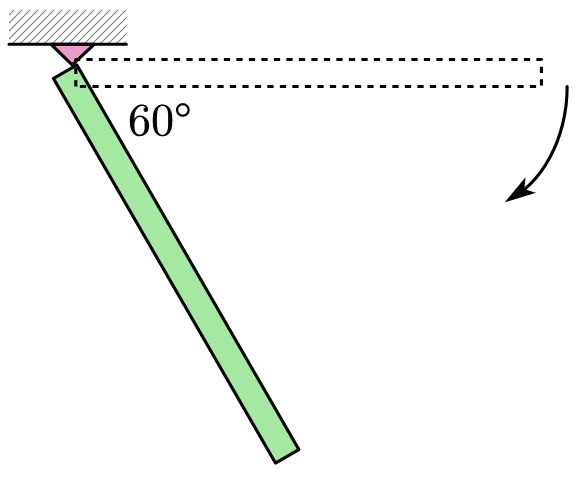
\includegraphics[width=\textwidth]{asset/ch4/T24.png}
    \end{minipage}

    \vspace{0.3em}

    \begin{minipage}{0.78\textwidth}

    (3)~要求转轴对细杆的力，可用质心运动定理。
    
    质心做圆周运动，需要切向和法向分别考虑。

    \vspace{0.3em}

    在沿杆方向上，$F_1-mg\sin{60^\circ}=m\omega^2\dfrac{l}{2}$，得$F_1=\dfrac{5\sqrt{3}}{4}mg$

    \vspace{0.5em}

    在垂直杆方向上，$mg\cos{60^\circ}-F_2=m\alpha\dfrac{l}{2}$，得$F_2=\dfrac{1}{8}mg$
    \end{minipage}
    \hfill
    \begin{minipage}{0.18\textwidth}
        \centering 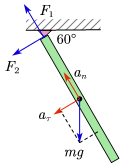
\includegraphics[width=\textwidth]{asset/ch4/T26.png}
    \end{minipage}

    

    \tcbline

    【补充练习】针对补充练习7的情景，在圆盘转过$90^\circ$时，求：(1)~圆盘转动的角加速度；(2)~转轴对圆盘的作用力。
\end{example}



\subsection{平面运动的刚体}

\noindent
\begin{minipage}{0.83\textwidth}
\setlength{\parindent}{2em}
\setlength{\parskip}{0.5em}
\linespread{1.3}

    对于做平面运动的刚体，其运动可以分解为整体随质心的平动和绕质心的转动。

    根据柯尼希定理，刚体的动能就等于这两项动能之和。
    
    \begin{formula}
        $E_k=\dfrac{1}{2}mv_C^2+\dfrac{1}{2}J\omega_C^2$
    \end{formula}
    
    \end{minipage}
    \hfill
    \begin{minipage}{0.15\textwidth}
        \centering 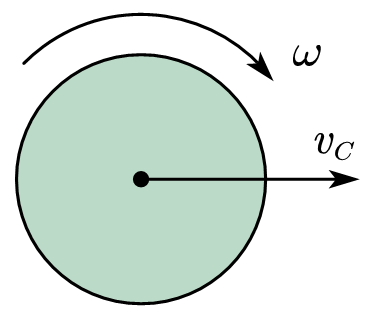
\includegraphics[width=\textwidth]{asset/ch4/T25.png}
    \end{minipage}

\begin{example}{平面运动的刚体*}
    长为$L$的均匀细杆竖直放在光滑地面上，从静止倒下，求杆滑到地面瞬间的质心速度。
    \tcblower
    
    \begin{minipage}{0.73\textwidth}

    杆在水平方向不受外力，因此质心速度一定竖直向下，设为$v$

    杆的A端在水平面上运动，在最终状态运动到最远点，速度为零。

    \vspace{0.3em}

    因此杆绕质心转动的角速度$\omega$满足$v=\omega \cdot \dfrac{L}{2}$

    \vspace{0.5em}
    
    整个过程只有重力做功，机械能守恒，$mg\dfrac{L}{2}=\dfrac{1}{2}mv^2+\dfrac{1}{2}J\omega^2$

    \vspace{0.5em}

    其中杆绕质心的转动惯量$J=\dfrac{1}{12}mL^2$，联立解得$v=\dfrac{\sqrt{3gL}}{2}$.
    \end{minipage}
    \hfill
    \begin{minipage}{0.25\textwidth}
        \centering 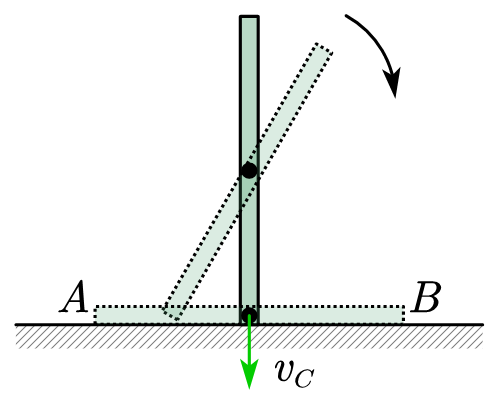
\includegraphics[width=\textwidth]{asset/ch4/T22.png}
    \end{minipage}
    
    \tcbline
    \begin{minipage}{0.82\textwidth}
    【补充练习】半径为$R$、质量为$m$的匀质实心球由静止沿斜面无滑动地滚动下来，求质心下降$h$时的速度大小。
    \end{minipage}
    \hfill
    \begin{minipage}{0.15\textwidth}
        %\vspace{-2em}
        \centering 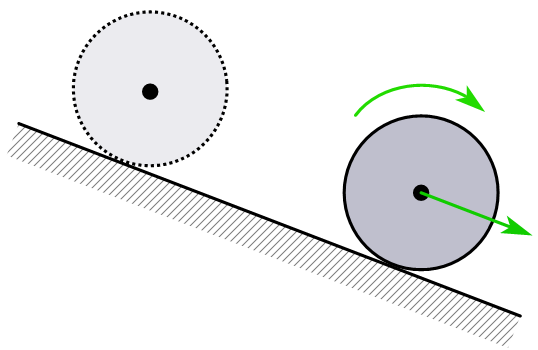
\includegraphics[width=\textwidth]{asset/ch4/T23.png}
    \end{minipage}
    
\end{example}

\subsection{连续受力的刚体}

\begin{example}{连续受力的刚体}
    长为$L$、质量为$m$的均匀细杆放在桌面上，绕中点在桌面上旋转。桌面与细杆的动摩擦因数为$\mu$. 求：(1) 细杆所受的摩擦力矩；(2) 细杆转动的角加速度。
    \tcblower
    (1)~将细杆切成长为$dx$的小段，每小段的质量为$m\dfrac{dx}{L}$，所受摩擦力为$\mu mg\dfrac{dx}{L}$
    
    对于到中点距离为$x$的小段，摩擦力矩为$\mu mg\dfrac{xdx}{L}$

    因此全长的摩擦力矩为$M=2\displaystyle\int_0^{L/2}{\mu mg\dfrac{xdx}{L}}=\dfrac{\mu mgL}{4}$

    (2)~细杆相对于中点的转动惯量为$J=\dfrac{1}{12}mL^2$，根据转动定律$M=J\alpha$，可得$\alpha=\dfrac{3\mu g}{L}$

    \tcbline

    【补充练习】半径为$R$、质量为$m$的均匀圆盘放在桌面上，绕圆心在桌面上旋转。桌面与圆盘的动摩擦因数为$\mu$. 若圆盘的初角速度为$\omega$，求停止之前转过的角度。
\end{example}

\colorlet{maincolor}{MainPurple}
\colorlet{sidecolor}{MainPurple!50}

\part{振动和波}

\chapter{机械振动}
\setcounter{example_counter}{1}

\section{简谐振动的描述}

\subsection{简谐振动的表达式}

\subsubsection{位移}

\noindent
\begin{minipage}{0.73\textwidth}
    \setlength{\parskip}{0.5em}
    \setlength{\parindent}{2em}
    \linespread{1.3}
    \textbf{简谐振动}：离开平衡位置的位移$x$按余弦规律随时间变化。

    以平衡位置为基准，简谐振动位移的通式为
    
\end{minipage}
\hfill
\begin{minipage}{0.25\textwidth}
    \centering 
\includegraphics[width=\textwidth]{asset/ch5/T1.png}
\end{minipage}

\vspace{0.5em}

\begin{formula}
    $x=A\cos (\omega t+ \varphi)$
\end{formula}

\begin{itemize}
    \item $A$称为振幅，$\omega$称为角频率（或圆频率）
    \vspace{0.25em}
    \item 周期$T=\dfrac{2\pi}{\omega}$，频率$\nu=\dfrac{1}{T}=\dfrac{\omega}{2\pi}$
    \vspace{0.25em}
    \item $\omega t+ \varphi$称为相位，$t=0$时的相位$\varphi$称为初相位
\end{itemize}

\subsubsection{速度与加速度}

将$x$对$t$求导，可得速度$v$，再求导可得加速度$a$.

\begin{formula}
    $v=-A\omega \sin(\omega t+ \varphi),~a=-A\omega^2 \cos (\omega t+ \varphi)$
\end{formula}

从表达式可以看出，加速度与位移成正比且反向，这是简谐振动的运动学特征。

\begin{example}{简谐振动的运动学}
    某简谐振动的表达式为$x=A\cos ⁡(\omega t+\varphi)$ (SI)，已知$t=0$时的位移为$\SI{0.04}{m}$，速度为$\SI{0.12}{m/s}$，加速度为$\SI{-0.36}{m/s^2}$，求$A,\omega,\varphi$的值（$A,\omega>0,~|\varphi|<\pi$）。

    \tcblower

    将简谐振动表达式对$t$两次求导，得速度$v=-\omega A\sin{(\omega t+\varphi)}$，加速度$a=-A\omega^2 \cos (\omega t+ \varphi)$

    在$t=0$时，$x=A\cos\varphi=0.04,~v=-A\omega\sin\varphi=0.12,~a=-A\omega^2 \cos\varphi=0.36$
    
    两两相除得$\omega=3,~\tan\varphi=-1$，结合$\cos\varphi>0,~\sin\varphi<0$的要求，$\varphi=-\dfrac{\pi}{4}$符合题意。

    \vspace{0.5em}

    将$\cos\varphi=\dfrac{\sqrt{2}}{2}$代入$x=A\cos\varphi=0.04$，可得$A=0.04\sqrt{2}$
    
    \tcbline

    【补充练习】已知简谐振动的表达式为$x=0.1\cos{\left(8\pi t+\dfrac{2\pi}{3}\right)}$（SI），求最大速度、加速度，并求首次回到平衡位置的时间。
    
\end{example}


\subsection{旋转矢量法}

一个匀速圆周运动质点，其在$x$轴上的投影就是简谐振动，而且速度和加速度在$x$方向上的分量，也与简谐振动相同。利用这一关系，可以用逆时针旋转的矢量表示振动。

利用逆时针旋转、长度等于振幅$A$的矢量表示简谐振动，这种方法称为\textbf{旋转矢量法}。初始角度就是初相位$\varphi$，只画出初始矢量的位置，称为\textbf{相量图}，非常适合确定初相位。

\vspace{-0.5em}

\begin{figure}[htb]
    \centering
    
\includegraphics[width=0.7\linewidth]{asset/ch5/T2.png}
\end{figure}

\vspace{-1em}

\begin{example}{简谐振动的表达式：旋转矢量法}
    已知简谐振动的振幅为$4$，周期为$2$. 当$t=0$时第一次通过$x=−2$处，且速度为正方向。求简谐振动的表达式（$A,\omega>0,~|\varphi|<\pi$），并求下一次通过$x=-2$位置的时间。

    \tcblower

    根据题意，$A=4,~T=2$，所以$\omega=\dfrac{2\pi}{T}=\pi$，简谐振动表达式为$x=4\cos{(\pi t+\varphi)}$

    如果直接将$t=0,~x=-2$代入表达式，会得到$\varphi=\pm\dfrac{2\pi}{3}$，还需根据速度方向进一步判断。

    \begin{minipage}{0.75\textwidth}
    
    而画出相量图，则可清楚看出初相位应该是第三象限角，应取$\varphi=-\dfrac{2\pi}{3}$

    可快速得出振动表达式为$x=4\cos{\left(\pi t-\dfrac{2\pi}{3}\right)}$

    根据向量图可知，下一次通过$x=-2$位置的相位是$\dfrac{2\pi}{3}$
    
    结合初相位，可知需要再等$\dfrac{4\pi}{3}$个相位。
    
    这相当于$\dfrac{4\pi/3}{2\pi}=\dfrac{2}{3}$个周期，因此再次通过$x=-2$的时间为$t=\dfrac{2}{3}T=\dfrac{4}{3}$

    \vspace{0.5em}
    
    \end{minipage}
    \hfill
    \begin{minipage}{0.22\textwidth}
        \vspace{-0.3em}
    
        \centering 
\includegraphics[width=\textwidth]{asset/ch5/T4.png}
    \end{minipage}

    \vspace{-1em}

    \tcbline

    【补充练习】已知简谐振动的图像如下图所示，求简谐振动的表达式。

    \vspace{-0.5em}

    \begin{center}
        
\includegraphics[width=0.35\textwidth]{asset/ch5/T3.png}
    \end{center} 
    
\end{example}

\subsection{相位关系}

若两个振动的频率相同，则相位差$\Delta \varphi=\varphi_2−\varphi_1$不变，习惯上：
\begin{itemize}
    \item 若$\Delta\varphi=0$（或$2k\pi$），则称两个振动\textbf{同相}；若$\Delta\varphi=\pi$（或$(2k+1)\pi$），则称两个振动\textbf{反相}
    \item 若$\Delta\varphi>0$，一般说振动2\textbf{领先}$\Delta\varphi$的相位；若$\Delta\varphi<0$，一般说振动2\textbf{落后}$\Delta\varphi$的相位
\end{itemize}

\begin{figure}[htb]
    \centering
    
\includegraphics[width=0.5\linewidth]{asset/ch5/T8.png}
\end{figure}

\begin{example}{简谐振动的表达式：相位关系}
    已知简谐振动的速度最大值为$4$，振幅为$2$，$t=0$时为速度最大值，且为正方向。
    
    (1)~求简谐振动的表达式。(2)~另一个振动与之反相，求其表达式。

    \tcblower
    
    \begin{minipage}{0.8\textwidth}
    
    (1)~根据题意，$A=2,~A\omega=4$，可得$\omega=2$

    根据$t=0$时取速度最大值，可画出右图所示的相量图，看出$\varphi=-\dfrac{\pi}{2}$

    因此简谐振动表达式为$x=2\cos{(2t-\dfrac{\pi}{2})}$
    
    \end{minipage}
    \hfill
    \begin{minipage}{0.18\textwidth}
    
        \centering 
\includegraphics[width=\textwidth]{asset/ch5/T6.png}
    \end{minipage}

    (2)~两个振动反相，则相位差为$\pi$，可得$\varphi_2=\dfrac{\pi}{2}$，因此表达式为$x=A\cos{(2t+\dfrac{\pi}{2})}$

    \tcbline

    【补充练习】两个质点做同振幅、同频率的简谐振动，在振动过程中，它们总在经过振幅一半的地方相遇，且运动方向相反。求他们的相位差。
    
\end{example}

\section{简谐振动的力与能量}

\subsection{简谐振动的动力学}

根据简谐运动的表达式，可知$a=-\omega^2 x$，加速度与位移正比且反向，这是简谐振动的的动力学特征。

结合牛顿第二定律，可知简谐振动的回复力与位移正比且反向。
\begin{formula}
    $F=-kx~~~\text{或}~~~m\dfrac{dx^2}{dt^2}=-kx$
\end{formula}

结合牛顿第二定律，$F=ma$，其中$a=-\omega^2 x$，可得简谐振动的角频率和周期为
\begin{formula}
    $\omega=\sqrt{\dfrac{k}{m}},~~T=2\pi\sqrt{\dfrac{m}{k}}$
\end{formula}

\subsection{简谐振动的能量}

\vspace{-1em}

\noindent
\begin{minipage}{0.78\textwidth}
    \setlength{\parskip}{0.5em}
    \setlength{\parindent}{2em}
    \linespread{1.3}
    在简谐振动的过程中，动能和势能相互转化，转化的过程中总能量不变。

    \begin{itemize}
        \item 在平衡位置，动能最大而势能为零
        \item 在位移最大处，动能为零而势能最大
    \end{itemize}
    
\end{minipage}
\hfill
\begin{minipage}{0.2\textwidth}
    \centering 
\includegraphics[width=\textwidth]{asset/ch5/T18.png}
\end{minipage}

%$E_k=\dfrac{1}{2}mv^2=\dfrac{1}{2}mA^2\omega^2\sin^2(\omega t+\varphi),~E_p=\dfrac{1}{2}kx^2=\dfrac{1}{2}kA^2\cos^2(\omega t+\varphi)$，结合$\omega=\sqrt{\dfrac{k}{m}}$，可得

%$E=E_k+E_p=\dfrac{1}{2}kA^2=\dfrac{1}{2}m\omega^2 A^2$

\begin{formula}
    $E=E_k+E_p=\dfrac{1}{2}mv^2+\dfrac{1}{2}kx^2=\dfrac{1}{2}kA^2=\dfrac{1}{2}m\omega^2 A^2$
\end{formula}

\begin{example}{简谐振动的能量}
    有一弹簧振子，弹簧劲度系数为$k=\SI{25}{N/m}$，振子振动的初动能为$\SI{2}{J}$，初势能为$\SI{6}{J}$.
    
    求：(1)~振幅；(2)~当位移是多大时，势能与动能相等。

    \tcblower

    

    (1)~总能量$E=E_k+E_p=\SI{8}{J}$，当振幅最大时，全为势能，$E=\dfrac{1}{2}kA^2$，得$A=\SI{0.8}{m}$

    (2)~势能与动能相等时，$E_p=\dfrac{1}{2}E=\SI{4}{J}$，利用$E_p=\dfrac{1}{2}kx^2$，得$x=0.4\sqrt{2}\unit{m}$

    \tcbline

    【补充练习】某弹簧振子重物的质量为$\SI{0.01}{kg}$，振动表达式$x=0.1\cos\left(8\pi t+\dfrac{2\pi}{3}\right)$（SI）.~求：(1)~弹簧的劲度系数；(2)~通过平衡位置时的速率；(3)~动能等于势能3倍时的位移。
    
\end{example}

\subsection{简谐振动的实例}

\subsubsection{弹簧振子}

弹簧振子的$A,\varphi$由初始条件确定，但角频率和周期只由系统本身决定。

\noindent
\begin{minipage}{0.73\textwidth}
    \setlength{\parskip}{0.5em}
    \setlength{\parindent}{2em}
    \linespread{1.3}
    弹簧振子的回复力是弹簧的弹力，满足$F=-kx$，所以是简谐振动。

    
    
\end{minipage}
\hfill
\begin{minipage}{0.25\textwidth}
    \centering 
\includegraphics[width=\textwidth]{asset/ch5/T1.png}
\end{minipage}

\begin{formula}
    $\dfrac{d^2x}{dt^2}=-\dfrac{k}{m}x,~~\omega=\sqrt{\dfrac{k}{m}},~~T=\dfrac{2\pi}{\omega}=2\pi\sqrt{\dfrac{m}{k}}$
\end{formula}

\note{若弹簧振子竖直放置，以平衡位置为基准，重力势能与弹性势能之和仍为$\dfrac{1}{2}kx^2$，所有结论仍成立。}

\begin{example}{弹簧振子}
    \begin{minipage}{0.73\textwidth}
        光滑水平面上的弹簧振子有质量为$M$的木块和劲度系数为$k$的弹簧构成。弹簧处于原长，一个质量为$m$的子弹以速度$u$射入木块并留在其中，系统开始振动。求振动方程（向右为正）。 
    \end{minipage}
    \hfill
    \begin{minipage}{0.25\textwidth}
        \centering 
\includegraphics[width=\textwidth]{asset/ch5/T10.png}
    \end{minipage}
    
    \tcblower

    

    在射入后瞬间，由动量守恒，$mu=(m+M)v$，此时系统能量为$E=E_k=\dfrac{1}{2}(M+m)v^2$

    振动过程中总能量不变，因此在振幅最大处，$E=E_p=\dfrac{1}{2}kA^2$，解得$A=\dfrac{mu}{\sqrt{k(M+m)}}$

    利用简谐运动的动力学公式，可得$\omega=\sqrt{\dfrac{k}{M+m}}$，利用旋转矢量法可知初相位$\varphi=-\dfrac{\pi}{2}$
    
    因此振动方程为$x=\dfrac{mu}{\sqrt{k(M+m)}}\cos\left(\sqrt{\dfrac{k}{M+m}}t-\dfrac{\pi}{2}\right)$

    \tcbline

    \vspace{-1em}
    
    \begin{minipage}{0.88\textwidth}
        【补充练习】劲度系数$\SI{10}{N/m}$的轻弹簧下端挂有质量为$\SI{1}{kg}$的盘子。现有质量也为$\SI{1}{kg}$的物体在高为$\SI{1}{m}$处自由下落，并与盘子粘在一起，系统开始振动。求振动方程。
    \end{minipage}
    \hfill
    \begin{minipage}{0.1\textwidth}
        \centering 
\includegraphics[width=\textwidth]{asset/ch5/T11.png}
    \end{minipage}
    
\end{example}

\subsubsection{单摆}

\noindent
\begin{minipage}{0.85\textwidth}
    \setlength{\parskip}{0.5em}
    \setlength{\parindent}{2em}
    \linespread{1.3}
    单摆的回复力是重力在切线方向的分力$mg\sin \theta$，若摆动幅度很小，可用小角近似$\sin \theta \sim \theta$，因此可认为回复力$F=-mg\theta$，与$\theta$正比且反向。这说明在摆角很小的情况下，单摆的运动是简谐振动。

    摆球的切向加速度$a_t=l\alpha=l\dfrac{d^2\theta}{dt^2}$，所以动力学方程为$ml\dfrac{d^2\theta}{dt^2}=-mg\theta$，据此可得

    \begin{formula}
        $\dfrac{d^2\theta}{dt^2}=-\dfrac{g}{l}\theta,~~\omega=\sqrt{\dfrac{g}{l}},~~T=2\pi\sqrt{\dfrac{l}{g}}$
    \end{formula}
    
\end{minipage}
\hfill
\begin{minipage}{0.12\textwidth}
    \centering 
\includegraphics[width=\textwidth]{asset/ch5/T12.png}
\end{minipage}

注意不要把单摆振动的相位与摆角混淆。
\begin{itemize}
    \item 最大摆角对应最大位移，相位为0和$\pi$
    \item 摆角为0对应平衡位置，相位为$、pm\dfrac{\pi}{2}$
\end{itemize}

\subsubsection{复摆}

\noindent
\begin{minipage}{0.83\textwidth}
    \setlength{\parskip}{0.5em}
    \setlength{\parindent}{2em}
    \linespread{1.3}
    绕不过质心的水平固定轴转动的刚体，称为复摆，需要用转动定律进行分析。

    在摆角很小的情况下，回复力矩$M=-mgl\sin\theta\sim -mgl\theta$，其中$l$表示质心到转轴的距离。回复力矩与$\theta$正比且反向，说明复摆的运动是简谐振动。
    
    利用转动定律，可列出振动的动力学方程$J\dfrac{d^2\theta}{dt^2}=-mgl\theta$，据此可得
    
\end{minipage}
\hfill
\begin{minipage}{0.15\textwidth}
    \centering 
\includegraphics[width=\textwidth]{asset/ch5/T13.png}
\end{minipage}

\begin{formula}
    $\dfrac{d^2\theta}{dt^2}=-\dfrac{mgl}{J}\theta,~~\omega=\sqrt{\dfrac{mgl}{J}},~T=\dfrac{2\pi}{\omega}=2\pi\sqrt{\dfrac{J}{mgl}}$
\end{formula}

\begin{example}{单摆与复摆}

    \begin{minipage}{0.85\textwidth}
        一均匀细圆环质量为$m$，半径为$R$，挂在墙上的钉子上。求微小摆动的周期。

        提示：圆环相对于钉子的转动惯量$J=2mR^2$.

    \end{minipage}
    \hfill
    \begin{minipage}{0.1\textwidth}
        \centering 
\includegraphics[width=\textwidth]{asset/ch5/T19.png}
    \end{minipage}

    \tcblower
    
    圆环若偏离很小的$\theta$角度，则回复力矩$M=-mgR\sin\theta \approx -mgR\theta$

    \vspace{0.5em}

    振动方程为$J\dfrac{d^2\theta}{dt^2}=-mgR\theta$，整理得$\dfrac{d^2\theta}{dt^2}=-\dfrac{g}{2R}\theta$.~因此$\omega=\sqrt{\dfrac{g}{2R}}$，$T=\dfrac{2\pi}{\omega}=2\pi \sqrt{\dfrac{2R}{g}}$
    \tcbline
    【补充练习】将一个单摆的摆球向负方向拉开很小的$\theta$角并放手，使之自由运动。它的初相位是多少？摆球首次来到平衡位置时的相位是多少？
\end{example}

\section{同方向简谐振动的合成}

\subsection{同方向同频率}

\noindent
\begin{minipage}{0.73\textwidth}
    \setlength{\parskip}{0.5em}
    \setlength{\parindent}{2em}
    \linespread{1.3}
    同方向、同频率的两个振动$x_1=A_1\cos{(\omega t+\varphi_1)},~x_2=A_2\cos{(\omega t+\varphi_2)}$，合成的结果仍然是同频率的简谐振动，参数可根据旋转矢量法进行确定。

    \begin{itemize}
    \item 若两个振动同相（$Δ\varphi=0$），则振幅最大，$A=A_1+A_2$
    \item 若两个振动反相（$Δ\varphi=\pi$），则振幅最小，$A=|A_1-A_2|$
    \item 其余情况，振幅$A$介于二者之间
\end{itemize}
\end{minipage}
\hfill
\begin{minipage}{0.25\textwidth}
    \centering 
\includegraphics[width=\textwidth]{asset/ch5/T14.png}
\end{minipage}

\begin{example}{同方向同频率的振动合成}
    有两个同方向的振动$x_1=4\cos⁡{(2t+\dfrac{\pi}{4})},~x_2=4\cos{⁡(2t+\dfrac{3\pi}{4})}$进行合成。 (1) 求合振动的方程；(2) 若还有第三个振动$x_3=3\cos⁡(2t+\varphi)$也参与合成，$\varphi$取何值时，合振动的振幅取得最大值和最小值，最大、最小值分别是多少？

    \tcbline

    %{\fangsong 同方向同频率振动合成的一般方法是旋转矢量法。}

    %\tcbline

    \begin{minipage}{0.76\textwidth}
        (1)~画出相量图可看出，合振动的振幅为$4\sqrt{2}$，初相位为$\dfrac{\pi}{2}$，频率不变。
    
        因此合振动方程为$x=4\sqrt{2}\cos{(2t+\dfrac{\pi}{2}})$
    
        (2)~要使合振动的振幅最大，应使振动同相，$\varphi=\dfrac{\pi}{2}$，最大振幅$A=4+3=7$

        \vspace{0.3em}
    
        要使合振动的振幅最小，应使振动反相，$\varphi=-\dfrac{\pi}{2}$，最大振幅$A=4-3=1$
    \end{minipage}
    \hfill
    \begin{minipage}{0.22\textwidth}
        \centering 
\includegraphics[width=\textwidth]{asset/ch5/T15.png}
    \end{minipage}

    \tcblower
    【补充练习】设有两个同方向简谐振动$x_1=A\cos(\omega t+\dfrac{\pi}{4}),~x_2=\sqrt{3}A\cos(\omega t+\dfrac{3\pi}{4})$. (1)~求合振动的表达式；(2)~再与第三个振动合成，使合振动的振幅达到$4A$，并让第三个振动的振幅尽可能小。

\end{example}

\subsection{同方向不同频率}
若两个振动的频率略有差异，合振动的振幅出现周期性变化，称为\textbf{拍}，拍频就是两个振动的频率之差。

\begin{formula}
    $\nu=|\nu_2-\nu_1|=\left|\dfrac{\omega_1}{2\pi}-\dfrac{\omega_2}{2\pi}\right|$
\end{formula}

%\begin{figure}[htb]
%    \centering
%    
\includegraphics[width=0.35\linewidth]{asset/ch5/T16.png}
%\end{figure}

\begin{example}{拍现象}
    音叉A与频率$\SI{415}{Hz}$的音叉B同时振动时，可在每秒内听到$2$拍。则音叉A与频率$\SI{420}{Hz}$的音叉C同时振动时，每秒内能听到几拍？
    \tcbline
    根据音叉A、B的振动可知，$|\nu_A-\nu_B|=\SI{2}{Hz}$，得$\nu_A=\SI{417}{Hz}$或$\SI{413}{Hz}$.

    因此音叉A、C振动时，拍频$\nu^\prime=|\nu_A-\nu_B|=\SI{3}{Hz}$或$\SI{7}{Hz}$.
    \tcbline
    【补充练习】一个$\SI{256}{Hz}$的音叉和待测音叉同时鸣响，若在$\SI{20}{s}$内听到$10$拍，求待测音叉的频率。
\end{example}

\section{拓展内容}

\subsection{简谐振动的判定}

要想判定一个运动是简谐振动，有以下三种等价的方法：
\begin{itemize}
    \item 受力特征：回复力与位移正比且反向，$F=-kx$
    \item 振动方程：$\dfrac{d^2x}{dt^2}+\omega^2x=0$（即$a=-\omega^2 x$）
    \item 能量特征：总能量不变，且势能$E_p=\dfrac{1}{2}kx^2$
\end{itemize}

\begin{example}{简谐振动的判定*}
    
    
    \begin{minipage}{0.8\textwidth}
    
    长为$l$、横截面积为$S$的木块浮在水面上，静止时浸没深度为$h$。将其稍向下压后松手，证明其之后的运动是简谐振动，并求振动周期。
    
    
    
    \end{minipage}
    \hfill
    \begin{minipage}{0.18\textwidth}
    
        \centering 
\includegraphics[width=\textwidth]{asset/ch5/T7.png}
    \end{minipage}

    

    \tcblower

    在平衡位置，浮力等于重力，$\rho_{\text{水}} gSh=\rho_{\text{木}}Slg$，得$\rho_{\text{水}}h=\rho_{\text{木}}l$

    以平衡位置为原点，向下为正。若向下压$x$的距离，则合力$F$等于重力减浮力。

    $F=\rho_{\text{木}}Slg-\rho_{\text{水}} gS(h+x)=-\rho_{\text{水}}gSx$，这说明回复力与位移成正比且反向，木块做简谐振动。

    对照简谐振动的动力学表达式，$k=\rho_{\text{水}}gS$，木块$m=\rho_{\text{木}}Sl$

    \vspace{0.5em}

    代入公式可得$\omega=\sqrt{\dfrac{k}{m}}=\sqrt{\dfrac{\rho_{\text{水}}gS}{\rho_{\text{木}}Sl}}=\sqrt{\dfrac{g}{h}}$，周期$T=\dfrac{2\pi}{\omega}=2\pi \sqrt{\dfrac{h}{g}}$
        
    \tcbline 

    \begin{minipage}{0.82\textwidth}
    
    【补充练习】横截面均匀的光滑U形管中有适量液体，液体的总长度为$L$，忽略摩擦和液体黏性。证明液面的小幅上下振动是简谐振动，并求出振动周期。
    
    \end{minipage}
    \hfill
    \begin{minipage}{0.15\textwidth}
        \vspace{-2em}
        \centering 
\includegraphics[width=\textwidth]{asset/ch5/T9.png}
    \end{minipage}
    

\end{example}

\subsection{阻尼振动与受迫振动}

\subsubsection{阻尼振动}

设自振频率$\omega_0$的系统在振动过程中，受到$f=-\gamma v$的阻力，记阻尼系数$\beta=\dfrac{\gamma}{2m}$

\begin{itemize}
    \item 若$\beta>\omega_0$，称为\textbf{过阻尼}，不能振动
    \item 若$\beta=\omega_0$，称为\textbf{临界阻尼}，恰好不能振动
    \item 若$\beta<\omega_0$，称为\textbf{欠阻尼}，可以振动
\end{itemize}

在欠阻尼的情况下，振动周期变长$T=\dfrac{2\pi}{\sqrt{\omega_0^2-\beta^2}}$，振幅和能量逐渐减小，$A=A_0 e^{-\beta t},~E=E_0 e^{-2\beta t}$.

振幅减小到$\dfrac{1}{e}$的时间称为时间常量（鸣响时间）$\tau=\dfrac{1}{2\beta}$

在鸣响时间内振动的次数的$2\pi$倍称为品质因数（Q值），$Q=2\pi\dfrac{\tau}{T}=\omega \tau$

\begin{example}{阻尼振动*}
    一单摆在空气中摆动，初始振幅为$5^\circ$.~若经过$\SI{100}{s}$，振幅减为$4^\circ$.~求：再经过多长时间，振幅减为$2^\circ$，并求出鸣响时间。
    \tcblower
    根据$A=A_0 e^{-\beta t}$，可得$t=\dfrac{1}{\beta}\ln{\dfrac{A_0}{A}}$.~代入$A_0=5^\circ,~A=4^\circ,~t=\SI{100}{s}$，可求出$\beta\approx \SI{2.2e-3}{s^{-1}}$
    
    再代入$A_0=4^\circ,~A=2^\circ$的数据，可得$t\approx \SI{310.7}{s}$.~进而鸣响时间$\tau=\dfrac{1}{2\beta}\approx \SI{448}{s}$
    \tcbline
    【补充练习】阻尼振动的起始振幅为$\SI{3.0}{cm}$，$\SI{10}{s}$后变为$\SI{1.0}{cm}$，再经过多长时间振幅变为$\SI{0.3}{cm}$.
\end{example}

\subsubsection{受迫振动}

在周期性驱动力的作用下，系统振动的频率等于驱动力的频率，而不是自振频率。

驱动力的频率与自振频率越接近，振幅越大。当二者相等时，振幅都达到最大值，称为\textbf{共振}现象。

\subsection{相互垂直的简谐振动合成}

%\subsubsection{相互垂直的简谐振动合成}

\vspace{-0.5em}

\noindent
\begin{minipage}{0.65\textwidth}
    \setlength{\parskip}{0.5em}
    \setlength{\parindent}{2em}
    \linespread{1.3}
    若质点在$x,y$方向的运动都是简谐运动，且频率相等，则合运动的轨迹是直线或椭圆，取决于相位差。
    
    \begin{itemize}
    \item 若相位差为$0$或$\pi$，则轨迹为直线
    \item 若$y$的相位比$x$领先，则为右旋的椭圆（顺时针转动）
    \item 若$y$的相位比$x$落后，则为左旋的椭圆（逆时针转动）
\end{itemize}
    
\end{minipage}
\hfill
\begin{minipage}{0.33\textwidth}
    \centering 
\includegraphics[width=\textwidth]{asset/ch5/T20.png}
\end{minipage}

\vspace{-0.5em}

\noindent
\begin{minipage}{0.78\textwidth}
    \setlength{\parskip}{0.5em}
    \setlength{\parindent}{2em}
    \linespread{1.3}
    若质点在$x,y$方向的运动都是简谐运动，且频率是简单的整数比，则质点合运动的轨迹是一个闭合曲线，称为\textbf{李萨如图形}。

    沿着闭合曲线，两个方向振动的频率之比，等于到达$x,y$最大位移的次数之比。若到达角点，则各算半次。
    
\end{minipage}
\hfill
\begin{minipage}{0.2\textwidth}
    \centering 
\includegraphics[width=\textwidth]{asset/ch5/T17.png}
\end{minipage}

%\begin{formula}
%    $\dfrac{\nu_x}{\nu_y}=\dfrac{x\text{方向最大位移次数}}{y\text{方向最大位移次数}}$
%\end{formula}

\note{若$x,y$方向的运动不成比例，则质点的运动轨迹不闭合，但很容易锁定到简单整数比。}

\begin{example}{李萨如图形*}
    \vspace{-0.5em}
    \begin{minipage}{0.88\textwidth}
        示波器的水平和垂直输入端分别加上余弦式交变电压，荧光屏上出现如图所示的曲线。已知水平方向振动频率为$\SI{2.7e4}{Hz}$，求垂直方向的振动频率。
        
    \end{minipage}
    \hfill
    \begin{minipage}{0.08\textwidth}
        \centering 
\includegraphics[width=\textwidth]{asset/ch5/T21.png}
    \end{minipage}
    \vspace{-0.5em}
    \tcblower

    \linespread{1.3}
    
    假想沿着曲线行走一圈，可以到达6次$x$最大位移和4次$y$最大位移，这说明在相同时间内，$x$方向振动了3个周期，而$y$方向只振动了2个周期，所以$\dfrac{\nu_x}{\nu_y}=\dfrac{6}{4}$，可得$\nu_y=\SI{1.8e4}{Hz}$
    
    \tcbline
    【补充练习】写出下列李萨如图形两个方向振动的频率之比。

    \begin{center}
        
\includegraphics[width=0.6\textwidth]{asset/ch5/T22.png}
    \end{center}
    
\end{example}

\chapter{机械波}
\setcounter{example_counter}{1}

\section{机械波的描述}

\subsection{基本概念}

\textbf{波动}是振动状态的传播，机械振动在介质中的传播称为\textbf{机械波}。

\note{振动是振动状态的传播，而不是介质本身的传播。}

机械波的产生要求有做机械振动的物体（\textbf{波源}），还要有连续的介质。

振动方向与传播方向垂直的称为\textbf{横波}，平行的称为\textbf{纵波}。

\begin{figure}[htb]
    \centering
    
\includegraphics[width=0.75\linewidth]{asset/ch6/T1.png}
\end{figure}

\vspace{-2.5em}

\subsection{特征量}

简谐振动的传播称为\textbf{简谐波}，是最简单的波。描述简谐波的特征量有：

\begin{itemize}
    \item 波速$u$：振动状态的传播速度，由介质决定
    \item 周期$T$：任意质元简谐振动的周期，也是一个完整波通过某点所需时间；频率$\nu$是周期的倒数
    \item 波长$\lambda$：相邻同相质元（相位差为$2\pi$）的距离
\end{itemize}

\note{其中波速$u$是振动状态的传播速度，并不是质元本身的运动速度。}

\begin{figure}[htb]
    \centering
    
\includegraphics[width=0.45\linewidth]{asset/ch6/T2.png}
\end{figure}

\vspace{-1em}

\subsection{波的传播规律}

经过一个周期，波刚好传播一个波长，因此简谐波特征量之间的关系为

\begin{formula}
    $u=\lambda \nu$
\end{formula}

沿波的传播方向，每隔一个波长$\lambda$，开始振动的时间落后一个周期$T$，相位落后$2\pi$，其比例关系为

\begin{formula}
    $\dfrac{\Delta \varphi}{2\pi}=\dfrac{\Delta x}{\lambda}=\dfrac{\Delta t}{T}$
\end{formula}

\begin{example}{简谐波的特征量}
    频率为$\SI{100}{Hz}$的简谐波以$\SI{300}{m/s}$的速度传播，振幅为$\SI{0.1}{m}$，依次经过相距$\SI{1}{m}$的质元A、B。
    
    求：(1)~波长；(2)~A的最大速度；(3)~A、B的相位差；(4)~当A处于负向最大位移时，B的位移。

    \tcblower

    (1)~波长$\lambda=\dfrac{u}{\nu}=\SI{3}{m}$；(2)~质元A振动的角速度$\omega=2\pi f$，最大速度为$v_m=A\omega=20\pi \unit{m/s}$

    (3)~每隔一个波长，相位落后$2\pi$，所以B落后的相位差$\Delta \varphi=\dfrac{\Delta x}{\lambda}\cdot 2\pi=\dfrac{2\pi}{3}$

    \vspace{0.3em}

    (4)~此时A相位$\varphi_A=\pi$，B的相位为$\varphi_B=\pi-\dfrac{2\pi}{3}=\dfrac{\pi}{3}$，位移为$x_B=A\cos\varphi_B=\SI{+0.05}{m}$

    \tcbline

    【补充练习】一平面简谐波的波速为$\SI{6}{m/s}$，波源振动的周期为$\SI{0.1}{s}$，在波的传播方向上有质元A、B，其距离小于一个波长，且振动的相位差为$\dfrac{5\pi}{6}$.~求：(1)~波长；(2)~A、B之间的距离。
    
\end{example}

\vspace{-0.8em}

\subsection{简谐波的波函数}

\vspace{-0.5em}

\subsubsection{波函数的形式}

简谐波的波函数以位置$x$和时间$t$作为变量，描述了各质元、各时间的振动位移。

\begin{formula}
    $y=A\cos\left[\omega\left(t\mp\dfrac{x}{u}\right)+\varphi_0\right]$或$y=A\cos\left(\omega t+\varphi_0\mp \dfrac{2\pi}{\lambda}x\right)$或$y=A\cos\left(\omega t+\varphi_0\mp kx\right)$
\end{formula}

\note{若波正向传播，则$\mp$符号应取负号；若波反向传播，则$\mp$符号应取正号。}

\begin{itemize}
    \item 第一种表达式的含义是，位于$x$处的质点，振动开始的时间落后了$\dfrac{x}{u}$
    \item 第二种表达式的含义是，位于$x$处的质点，相位落后了$\dfrac{2\pi}{\lambda}x$
    \item 第三种表达式定义了角波数$k=\dfrac{2\pi}{\lambda}$，那么位于$x$处的质点，相位落后了$kx$
\end{itemize}

\vspace{-0.3em}

\begin{example}{波函数的含义}
    已知一列简谐波的波函数为$y=A\cos\pi(4t+2x)$（SI）。求：(1)~波长、频率、波速，判断传播方向；(2)~当$t=\SI{4.2}{s}$时，离原点最近的波峰；(3)~$t=\SI{4.2}{s}$之后，第一个波峰通过原点的时间。
    \tcblower

    \vspace{-0.3em}
    
    (1)~根据波函数可知$\omega=4\pi$，所以周期$T=\dfrac{2\pi}{\omega}=\SI{0.5}{s}$，频率$\nu=\dfrac{1}{T}=\SI{2}{Hz}$

    波函数中$x$的系数是$\dfrac{2\pi}{\lambda}$，可得$\lambda=\SI{1}{m}$，进而$u=\lambda\nu=\SI{2}{m/s}$
    
    $x$的系数为正号，说明波向$-x$方向传播。

    (2)~当$t=\SI{4.2}{s}$时，$y=A\cos\pi(16.8+2x)$，波峰应满足$\pi(16.8+2x)=2k\pi (k\in \mathbb{Z})$，即$x=k-8.4$，当$k=8$时，$x=\SI{-0.4}{m}$，这是离原点最近的波峰。

    (3)~令$x=0$，则$y=A\cos 4\pi t$，波峰应满足$4\pi t=2k\pi (k\in \mathbb{Z})$，即$t=0.5 k$，当$k=9$时，$t=\SI{4.5}{s}$，这是$\SI{4.2}{s}$之后第一个符合条件的时刻。
    \tcbline
    【补充练习】一列简谐波的波函数为$y=0.05\cos(10\pi t-4\pi x)$（SI）。求：(1)~波长、频率、波速，判断传播方向；(2)~求各质元振动的最大速度和最大加速度；(3)~$x=\SI{1}{m}$处质点来到平衡位置的所有时刻；(4)~$t=\SI{0.2}{s}$时所有波峰的位置。
\end{example}

%将波函数沿波的传播方向移动一小段距离，即可判断各质点的速度方向。

\subsubsection{波函数的求解}

在求解波函数时，可分以下三步：
\begin{itemize}
    \item 先求出任意一点（例如$x_0$处）的振动函数为$y=A\cos(\omega t+\varphi)$
    \item 求出波的特征量（我喜欢用波长$\lambda$），并判断波的传播方向
    \item 利用每隔一个波长$\lambda$，相位落后$2\pi$对相位进行调整，得到波函数$y=A\cos\left(\omega t+\varphi\mp 2\pi\cdot \dfrac{x-x_0}{\lambda}\right)$
\end{itemize}

\begin{example}{波函数的求解}
    一列简谐波向$x$轴正方向传播，振幅$\SI{10}{cm}$，频率$\SI{10}{Hz}$，波长大于$\SI{10}{cm}$。在$t=\SI{1}{s}$时刻，$x=\SI{10}{cm}$处的A质元通过平衡位置且向负方向运动；而$x=\SI{20}{cm}$处的B质元位移为$y=\SI{5}{cm}$且向正方向运动。求：(1)~A、B两点的相位差；(2)~波长；(3)~波函数。

    \tcblower
    
    (1)~根据旋转矢量法，$t=\SI{1}{s}$时刻，A的相位为$\dfrac{\pi}{2}$，B的相位为$-\dfrac{\pi}{3}$，B落后A的相位为$\dfrac{5\pi}{6}$

    \vspace{0.3em}

    (2)~根据波的传播规律，距离相差$\lambda$，相位就落后$2\pi$

    \vspace{0.5em}
    
    根据这个比例关系，$\dfrac{x_B-x_A}{\lambda}=\dfrac{5\pi/6}{2\pi}$，得波长$\lambda=\SI{0.24}{m}$

    \vspace{0.5em}
    
    (3)~先求A质元的振动方程，根据频率和振幅，可得$x_A=0.1 \cos{\left(7\pi t+\varphi \right)}$

    \vspace{0.5em}

    在$t=\SI{1}{s}$时刻，相位$\left(7\pi t+\varphi \right)=\dfrac{\pi}{2}$，求得初相位$\varphi=-\dfrac{\pi}{2}$，所以$y_A=0.1 \cos{\left(7\pi t-\dfrac{\pi}{2} \right)}$

    \vspace{0.5em}

    最后调整为波函数$y=0.1 \cos{\left(7\pi t-\dfrac{\pi}{2} -2\pi\cdot \dfrac{x-0.1}{\lambda}\right)}=0.1 \cos{\left(7\pi t-\dfrac{25\pi}{3} x+\dfrac{\pi}{3}\right)}$
    
    \tcbline
    
        【补充练习】已知$t=0$和$t=\SI{0.5}{s}$时，波形图分别为实线和虚线，已知周期$T>\SI{0.5}{s}$，求波函数。
   
    \begin{center}
        
\includegraphics[width=0.35\textwidth]{asset/ch6/T5.png}
    \end{center}
    
\end{example}

\subsubsection{波形图}

波函数同时表达了$y$与$x,t$的关系：
\begin{itemize}
    \item 若固定某一个位置$x$，则波函数表达了该位置质元振动的位移$y$与时间$t$的关系，可画出振动图像
    \item 若固定某一个时刻$t$，则波函数表达了该时刻各质元的振动位移$y$，可画出波形图
\end{itemize}

\begin{figure}[htb]
    \centering
    
\includegraphics[width=0.65\linewidth]{asset/ch6/T3.png}
\end{figure}

\begin{example}{波形图与振动图像}
    一列简谐波在$t=\SI{2}{s}$时的波形图和$x=\SI{5}{m}$处质点的振动图像如图所示。
    
    (1)~判断波的传播方向；(2)~求波速；(3)~求波函数；(4)~求$x=0$处的质元在$t=0$时的速度.

    \vspace{-0.5em}

    \begin{center}
        
\includegraphics[width=0.6\textwidth]{asset/ch6/T6.png}
    \end{center}

    \tcblower
    
    (1)~在振动图像上，$x=\SI{5}{m}$处的质点在$t=\SI{2}{s}$时，位于平衡位置，且向正方向运动。

    在波形图上，若图像向左微小平移，可以实现该位置向上运动，因此波向$-x$方向传播。

    (2)~根据波形图可知$\lambda=\SI{12}{m}$，根据振动图像可知周期$T=\SI{8}{s}$，所以波速$u=\lambda\nu=\lambda/T=\SI{1.5}{m/s}$

    \vspace{0.5em}

    (3)~先写出$x=\SI{5}{m}$处质点的振动方程为$y=10\cos{\left(\dfrac{\pi}{4}t+\pi\right)}$

    \vspace{0.5em}

    再结合波长和传播方向，可写出波函数为$y=10\cos{\left(\dfrac{\pi}{4}t+\pi+2\pi\dfrac{x-5}{12}\right)}=10\cos\pi\left(\dfrac{t}{4}+\dfrac{x}{6}+\dfrac{1}{6}\right)$

    \vspace{0.5em}

    (4)~将$x=0$代入波函数，得振动方程$y=10\cos\pi\left(\dfrac{t}{4}+\dfrac{1}{6}\right)$

    \vspace{0.5em}

    求导可得速度表达式$v=-\dfrac{5\pi}{2}\sin\left(\dfrac{t}{4}+\dfrac{1}{6}\right)$.~当$t=0$时，速度$v=-\dfrac{5}{4}\pi~\unit{m/s}$
    
    \tcbline

     \begin{minipage}{0.7\textwidth}
        【补充练习】一列平面简谐波以$\SI{4}{m/s}$的速度向$x$正方向传播。

        (1)~若右图表示$x=0$处质元的振动图像，求波函数；
        
        (2)~若右图表示$t=0$时的波形图，求波函数。
    \end{minipage}
    \hfill
    \begin{minipage}{0.27\textwidth}
        \centering 
\includegraphics[width=\textwidth]{asset/ch6/T7.png}
    \end{minipage}
\end{example}

\section{波的能量}

\subsection{变化规律}

能量可以随着波动而传播，在简谐波中，每一质元的动能和势能同时变化，且任意时刻都相等。

\begin{itemize}
    \item 在平衡位置，动能、势能都达到最大值
    \item 在波峰、波谷，动能、势能都为零
\end{itemize}

\warn{在机械振动中，动能和势能的变化是反向的；而在简谐波中，动能和势能的变化是同向的。}

\subsection{定量关系}

介质单位体积内的能量称为波的能量密度$w$，若介质的密度为$\rho$，则\textbf{平均能量密度}$\bar{w}=\dfrac{1}{2}\rho \omega^2A^2$.

单位时间通过面积$S$的能量称为\textbf{能流}。通过垂直于波传播方向上单位面积能流的时间平均值，称为\textbf{波的强度}$I=\bar{w}u$，就等于\textbf{平均能流密度}。

\vspace{-0.5em}

\begin{formula}
    $\bar{w}=\dfrac{1}{2}\rho \omega^2A^2,~~~I=\bar{w}u$
\end{formula}

\note{从公式中可以看出，振动频率越大、振幅越大，则波的能量密度就越大。}

\begin{example}{波的能量}
    一列简谐横波在张紧的弦上传播，波函数为$y=0.02\cos(4\pi x−200\pi t)$（SI）

    (1)~判断波的传播方向，并求出波长和波速。(2)~在$x=0$的质元，什么时候能量最小？(3)~在$t=0$时刻，哪里的质元能量最大？(4)~若弦的线密度为$\SI{8e-3}{kg/m}$，求波的平均能量密度和波的强度。

    \tcblower

    (1)~发现$t$前面的系数是负号，应先用诱导公式变形，$y=0.02\cos(200\pi t-4\pi x)$

    \vspace{0.3em}
    
    此时$x$前面的系数是负号，说明波向$x$正方向传播。$x$的系数是$\dfrac{2\pi}{\lambda}=4\pi$，得波长$\lambda=\SI{0.5}{m}$

    \vspace{0.2em}

    角频率$\omega=200\pi~\unit{s^{-1}}$，频率$\nu=\dfrac{\omega}{2\pi}=\SI{100}{Hz}$，所以波速$u=\lambda\nu=\SI{50}{m/s}$

    (2)~波峰和波谷的能量最小，代入$x=0$，应有$200\pi t=k\pi~(k\in\mathbb{Z})$，解得$t=\dfrac{k}{200}~\unit{s}~(k\in\mathbb{Z})$

    \vspace{0.5em}

    (3)~平衡位置的能量最大，代入$t=0$，应有$4\pi x=\dfrac{\pi}{2}+k\pi~(k\in\mathbb{Z})$，解得$t=\left(\dfrac{\pi}{8}+\dfrac{k}{4}\right)~\unit{s}~(k\in\mathbb{Z})$

    \vspace{0.2em}

    (4)~将$\rho=\SI{8e-3}{kg/m},~\omega=200\pi~\unit{s^{-1}},~A=\SI{0.02}{m},~u=\SI{1}{m/s}$代入公式

    \vspace{0.5em}

    得平均能量密度$\bar{w}=\dfrac{1}{2}\rho \omega^2A^2\approx \SI{0.63}{J/m}$，平均能流密度$I=\bar{w}u\approx \SI{31.6}{W}$
    
    \tcbline
    【补充练习】关于机械波，判断下列说法是否正确：(i)~各质元做简谐振动，动能与势能相互转化，机械能守恒；(ii)~动能最大的质元，势能也最大；(iii)~处于平衡位置的质元，动能最大、势能为零；(iv)~各质元将自己的能量传递给相邻质元，能量在传播过程中逐渐减小
\end{example}

\section{干涉与衍射}

\subsection{惠更斯原理与衍射}

\subsubsection{惠更斯原理}

媒质中任意波面上的各点，都可看作是发射子波的波源，其后的任一时刻，这些子波面的包络面就是波在该时刻的新的波面。

\subsubsection{衍射}

衍射是波传播遇到障碍物时，能绕过障碍物的边缘而偏离直线传播的现象。

相对波长而言，障碍物线度越小，衍射现象越明显。

\vspace{-0.5em}

\begin{figure}[htb]
    \centering
    
\includegraphics[width=0.78\linewidth]{asset/ch6/T8.png}
\end{figure}

\subsection{波的叠加与干涉}

%\subsubsection{波传播的独立性}
\subsubsection{波的叠加原理}

几列波可以保持各自特点同时通过同一介质，不受其它波的影响。

在几列波相遇而互相交叠的区域中，某点的振动是各列波单独传播时在该点引起的振动的合成。

\vspace{-0.8em}

\begin{figure}[htb]
    \centering
    
\includegraphics[width=0.6\linewidth]{asset/ch6/T11.png}
\end{figure}

\vspace{-1.2em}

\subsubsection{波的干涉}

波叠加时在空间出现稳定的振动加强和减弱的分布叫波的干涉。

波的干涉需要满足\textbf{相干条件}，即两列波频率相同、振动方向相同、相位差固定。

\note{这隐含了两列波的波长一定相等，但振幅不一定相同。}

\subsubsection{相长干涉与相消干涉}

若波源$S_1,~S_2$产生两列相干波，初相位之差为$\Delta \varphi_0$，到$P$点的距离差为$\Delta r$，则在$P$点的相位差为

\noindent
\begin{minipage}{0.81\linewidth}
    \begin{formula}
        $\Delta \varphi=\Delta \varphi_0-2\pi \dfrac{\Delta r}{\lambda}$
    \end{formula}
    
    \begin{itemize}
        \item 当$\Delta \varphi=2k\pi$（同相）时，是干涉加强点（相长干涉），振幅是两者之和
        \item 当$\Delta \varphi=(2k+1)\pi$（反相）时，是干涉减弱点（相消干涉），振幅是两者之差
    \end{itemize}
\end{minipage}
\hfill
\begin{minipage}{0.16\linewidth}
    \centering 
\includegraphics[width=\linewidth]{asset/ch6/T10.png}
\end{minipage}

\note{若波源同相，可直接用距离差$\Delta r$判定。若P点到波源距离之差为波长的整数倍$\Delta r=k\lambda~(k\in\mathbb{Z})$，则为相长干涉；若为半波长的奇数倍$\Delta r=(k+\dfrac{1}{2})\lambda~(k\in\mathbb{Z})$，则为相消干涉。}

\begin{example}{波的干涉——相位关系}
    $S_1,~S_2$是相干波源，发出波长为$\SI{2}{m}$的简谐波。它们到P点的距离分别为$\SI{4}{m},~\SI{4.4}{m}$.~已知$S_1$的振动方程为$y_1=\cos{(2\pi t+\pi)}$，$S_2$的振幅为$\SI{2}{m}$.~(1)~求波速；(2)~若P点为相长干涉，求$S_2,~P$的振动方程；(3)~若P点为相消干涉，求$S_2,~P$的振动方程。

    \tcblower

    {\fangsong 思路：首先根据相干条件判断频率相同，再根据干涉情况确定相位。}

    \tcbline
    (1)~根据振动方程，可知角频率$\omega=2\pi$，频率$\nu=\dfrac{\omega}{2\pi}=1$，所以波速$u=\lambda\nu=\SI{2}{m/s}$

    \vspace{0.3em}

    (2)~设$S_2$的振动初相为$\varphi_2$，代入公式可知，两列波在P点的相位差为$\Delta \varphi=(\varphi_2-\pi)-\dfrac{2\pi}{5}=\varphi_2-\dfrac{7\pi}{5}$

    若为相长干涉，则$\Delta \varphi=2k\pi$，可取$\varphi_2=-0.6\pi$，因此$S_2$振动方程为$y_2=2\cos{(2\pi t-0.6\pi)}$

    P点的振幅为二者之和，相位与$S_1$相同，可直接写出$y_P=3\cos{2\pi t+\pi}$

    (3)~若为相长干涉，则$\Delta \varphi=(2k+1)\pi$，可取$\varphi_2=0.4\pi$，因此$S_2$振动方程为$y_2=2\cos{(2\pi t+0.4\pi)}$

    P点的振幅为二者之差，相位与$S_1$相反，可直接写出$y_P=\cos{(2\pi t)}$

    \tcbline

    【补充练习】$S_1,~S_2$是相干波源，相距$\SI{3}{m}$，波长均为$\SI{2}{m}$，已知$S_1$的初相是$\pi/2$。分别在以下条件下求$S_2$的初相。(1)~$S_1S_2$的中垂线各点均为相消干涉；(2)~$S_1S_2$的延长线上各点均为相消干涉。
\end{example}

\begin{example}{波的干涉——加强/减弱点的数量}
    两相干波源$S_1,~S_2$在$x$轴上的位置为$x=\SI{0}{m}$和$x=\SI{45}{m}$，波长均为$\SI{20}{m}$.~已知$S_1$比$S_2$超前$\pi/2$个相位。求：(1)~在$x$轴上，所有相长和相消干涉的点的坐标；(2)~在以原点为圆心，$\SI{35}{m}$为半径的圆上，共有几个振动加强点和减弱点？

    \tcblower
    {\fangsong 思路：如果波源不是同相，要使用相位关系进行判断。}
    \tcbline

    (1)~设点P到波源的距离是$r_1,r_2$，不妨假设波到达P点时，$S_1$的相位就是$\pi/2$，$S_2$的相位是$0$.

    \vspace{0.5em}

    则波源$S_1$的波到达P点时，相位落后$\dfrac{2\pi}{\lambda}r_1$，变成$\dfrac{\pi}{2}-\dfrac{2\pi}{\lambda}r_1$
    
    \vspace{0.5em}
    
    同理波源$S_2$的波到达P点时，相位变成$-\dfrac{2\pi}{\lambda}r_2$，两者之差为$\Delta \varphi=\dfrac{\pi}{2}+\dfrac{\pi}{10}(r_2-r_1)$

    \vspace{0.5em}

    振动加强点和减弱点应满足$\Delta \varphi=2k\pi$和$(2k+1)\pi$，即$r_2-r_1=20k-5$和$20k+5~(k\in\mathbb{Z})$

    \begin{itemize}
        \item 在波源之间，设坐标为$x~(0<x<45)$，则$r_2-r_1=45-2x$.~代入条件得$x=5,15,25,35$是加强点，$x=10,20,30,40$是减弱点
        \item 在$S_2$右侧，$r_2-r_1=-45$，都是加强点；在$S_1$左侧，$r_2-r_1=45$，都是减弱点
    \end{itemize}

    (2)~在这个圆上，$r_1=35$，$r_2$的取值为$10\sim 80$

    当$r_2-r_1=20k-5$时是加强点，可取$r_2=10,30,50,70$.~注意$r_2=10$只有一个点符合条件，而其他在上半圆和下半圆各有一个，所以共7个加强点。

    当$r_2-r_1=20k+5$时是减弱点，可取$r_2=20,40,60,80$.~注意$r_2=80$只有一个点符合条件，而其他在上半圆和下半圆各有一个，所以共6个减弱点。
    
    \tcbline
    
    【补充练习】两相干波源$S_1,~S_2$在$x$轴上的位置为$x=\SI{0}{m}$和$x=\SI{30}{m}$，$x=\SI{9}{m}$和$\SI{12}{m}$处的两点是相邻的两个因干涉而静止的点。求两波的波长和两波源的相位差。

\end{example}

\subsection{多普勒效应}

由于波源(S)或观察者(R)的运动，接收到的频率$\nu_R$不同于波源频率$\nu_S$的现象，称为多普勒效应。

利用波速$u$，可推导出$\nu_R$与$\nu_S$的关系为

\begin{formula}
    $\nu_R=\dfrac{u+v_R}{u-v_S}\nu_S$
\end{formula}

波源和观察者的速度$v_S,v_R$的符号规定为，靠近彼此运动的方向为正，远离彼此的方向为负。

\note{这一公式可能有不同的写法，区别在于速度的正负规定不同。}

\note{若速度方向与波源、观察者的连线不共线，只考虑在连线上的分量。}

\begin{figure}[htb]
    \centering
    
\includegraphics[width=0.5\linewidth]{asset/ch6/T9.png}
\end{figure}

\begin{example}{多普勒效应}
    一警车追赶摩托车，两者在同一直路上行驶。警车的速度为$\SI{30}{m/s}$，发出频率为$\SI{400}{Hz}$的警笛，摩托车的速度为$\SI{20}{m/s}$，设空气中声速为$\SI{340}{m/s}$。
    
    %同时，空中一架飞机以$\SI{180}{m/s}$的速度行驶，发出频率为$\SI{1000}{Hz}$的声音。
    
    (1)~求静止在地面的观测者在警车前和警车后听到的声音频率；(2)~求摩托车司机听到的声音频率。
    
    %(3)~若有$\SI{10}{m/s}$的风向前吹，第(1)问的结果会如何变化？
    
    (3)~空中一架飞机以$\SI{180}{m/s}$的速度行驶，发出频率为$\SI{1000}{Hz}$的声音。当飞机与静止观测者的连线与地面成$60^\circ$和$90^\circ$角时，求他听到飞机声音的频率。

    \tcblower

    (1)~警车前方的观察者认为警车靠近自己，$v_S=+\SI{30}{m/s}$，代入公式可得$\nu_R=\dfrac{u}{u-v_S}\nu_S\approx \SI{439}{Hz}$

    \vspace{0.3em}

    而警车后方的观察者认为警车远离自己，$v_S=-\SI{30}{m/s}$，代入公式可得$\nu_R=\dfrac{u}{u-v_S}\nu_S\approx \SI{368}{Hz}$

    \vspace{0.3em}

    (2)~将$v_S=+\SI{30}{m/s},~v_R=-\SI{20}{m/s}$代入公式，可得$\nu_R=\dfrac{u+v_R}{u-v_S}\nu_S\approx\SI{413}{Hz}$

    \vspace{0.3em}

    %(3)~空气中的声速应理解为声波相对于空气的速度，如果有风，则要用相对运动的公式叠加。

    %声音向前方传播时，与风速相同，速度应相加，相对于观察者的速度是$u^\prime=\SI{350}{m/s}$

    %同理，声音向后方传播时，与风速相反，速度应相减，相对于观察者的速度是$u^\prime=\SI{330}{m/s}$

    %代回第(1)问公式可得$\nu_R$分别变为$\SI{434}{Hz}$和$\SI{364}{Hz}$.

    (3)~若飞机与观测者连线与地面成$60^\circ$角时，飞机在连线上的速度为$\SI{180}{m/s}\times \cos{60^\circ}=\SI{90}{m/s}$

    \vspace{0.3em}

    当飞机在自己后方时，飞机靠近自己，速度取正号，$\nu_R=\dfrac{u}{u-v_S}\nu_S= \SI{1360}{Hz}$

    \vspace{0.3em}

    当飞机在自己后方时，飞机靠近自己，速度取负号，$\nu_R=\dfrac{u}{u-v_S}\nu_S= \SI{791}{Hz}$

    \vspace{0.3em}

    若飞机与观测者连线与地面成$90^\circ$角，飞机在连线上速度为零，听到频率仍为$\SI{1000}{Hz}$

    \tcbline
    
    【补充练习】一静止声源S的频率为$\nu_S=\SI{300}{Hz}$，声速$u=\SI{330}{m/s}$，观察者R以速度$v_R=\SI{60}{m/s}$向右运动。在观察者右侧有一个反射壁，以速度$v=\SI{100}{m/s}$向右运动。此时，观测者会同时接收到直接来自声源和反射壁反射的声音，但二者频率不同，求观察者测得的拍频。
    （提示：可认为墙壁作为接收者接收声音后，又作为运动的发射者以相同频率发射声音。）
\end{example}

\section{拓展内容}

\subsection{驻波}

\subsubsection{驻波的概念}

两列相干的行波沿相反方向传播而叠加时，就形成\textbf{驻波}，这是一种重要的干涉现象。

\subsubsection{驻波的描述}

假设两列波的波函数分别为$y_1=A\cos(\omega t-kx),~~y_2=A\cos(\omega t+kx)$

\begin{formula}
    和差化积公式：$\cos\alpha+\cos \beta=2\cos\dfrac{\alpha+\beta}{2}\cos\dfrac{\alpha-\beta}{2}$
\end{formula}

根据和差化积公式，可得合成结果为

\begin{formula}
    $y=y_1+y_2=2A\cos{kx}\cdot \cos \omega t$
\end{formula}

这个实际是一个振动方程，$|2A\cos{kx}|$表示振幅，$\omega t$是相位。

由此可见，不同位置的振幅不同，某些位置振幅最大为$2A$，某些位置振幅为零。

\begin{example}{驻波的描述}
    在弦上有一驻波，其表达式为$y=0.02\cos{20x}\cos{750t}$.~(1)~求两个相邻波节的距离；(2)~这个驻波是哪两列波叠加而成的？给出波动方程。
    \tcblower
    (1)~驻波的振幅是$|0.02\cos{20x}|$，波节处振幅最小，即$20x=\dfrac{\pi}{2}+k\pi$，得$x=\dfrac{\pi}{40}+\dfrac{k\pi}{20}~(k\in \mathbb{Z})$

    \vspace{0.3em}
    
    因此相邻波节之间的距离是$\pi/20$

    \vspace{0.4em}

    (2)~根据积化和差公式，$y=0.01\cos{(750t+20x)}+0.01\cos{(750t-20x)}$，这就是两列波的方程。
    
    \tcbline
    【补充练习】两列简谐波沿$x$轴传播，波动方程为$y=A\cos{2\pi(t-x)}$和$y=A\cos{2\pi(t+x)}$，叠加形成驻波。(1)~求波节的位置坐标；(2)~求波腹的振幅。
\end{example}

\subsubsection{驻波的特点}

\begin{itemize}
    \item 振幅：不等大，振幅最大处称为波腹，振幅最小处称为波节，相邻波节间距离为$\dfrac{\lambda}{2}$。
    \item 相位：两个波节内部的各点相位相同，一个波节两侧各点相位相反
    \item 能量：驻波不传播能量，只在相邻波节和波腹之间有能量交换
\end{itemize}

\note{如果两列波振幅不相等，也能称为驻波，只是波节处仍有振动。}

\vspace{-0.5em}

\begin{figure}[htb]
    \centering
    
\includegraphics[width=0.35\linewidth]{asset/ch6/T13.png}
\end{figure}

\vspace{-1em}

\subsection{波的反射与驻波}

\subsubsection{波的反射}

驻波常由反射前后的波叠加形成，波在反射前后，除了传播方向相反，相位也可能会发生变化。
\begin{itemize}
    \item 波在\textbf{固定端}的反射前后，相位会突变$\pi$，称为\textbf{半波损失}
    \item 波在\textbf{自由端}的反射前后，相位没有变化，没有半波损失的现象。
\end{itemize}

若反射前后的波叠加形成驻波，在固定端一定是波节，自由端一定是波腹。

\begin{figure}[htb]
    \centering
    
\includegraphics[width=0.55\linewidth]{asset/ch6/T14.png}
\end{figure}

%\vspace{-1.3em}

\subsubsection{界面处的反射}

若波从一种介质传播到另一种介质，将同时发生反射和透射，透射都不会发生相位变化，但反射要看两种介质的性质。
\begin{itemize}
    \item 若波从波疏介质传播到波密介质（轻绳到密绳），相当于固定端，反射时有半波损失，相位突变$\pi$
    \item 若波从波密介质传播到波疏介质（密绳到轻绳），相当于自由端，反射时相位不变
\end{itemize}

\begin{figure}[htb]
    \centering
    
\includegraphics[width=0.7\linewidth]{asset/ch6/T15.png}
\end{figure}

\vspace{-1em}

\begin{formula}
    在求解反射波方程时，若波在$x=d$处反射，用$2d-x$替换原来的$x$，若有半波损失，再加$\pi$即可。
\end{formula}

\begin{example}{因反射形成的驻波}
    一平面简谐波沿$x$轴正方向传播，在$x=3\lambda /4$处遇到界面而反射。设入射波和反射波的振幅均为$A$，频率为$\nu$.~已知在$t=0$时，原点处的合振动是经过平衡位置向负方向运动。
    
    (1)~判断波是从波疏介质传播到波密介质，还是从波密介质传播到波疏介质；
    
    (2)~求$x=7\lambda/12$处，入射波与反射波的合振动方程。

    \tcblower

    (1)~先写出入射波方程$y_1=A\cos{(2\pi \nu t-\dfrac{2\pi}{\lambda}x+\varphi_0)}$，要求反射波方程，就把$x$替换成$2\cdot \dfrac{3}{4}\lambda-x$

    \vspace{0.5em}
    
    假设没有半波损失，则$y_2=A\cos{[2\pi \nu t-\dfrac{2\pi}{\lambda}(2\cdot \dfrac{3}{4}\lambda-x)+\varphi_0]}=A\cos{(2\pi \nu t+\dfrac{2\pi}{\lambda}x+\varphi_0-\pi)}$

    \vspace{0.5em}

    利用和差化积公式，二者叠加的结果是$y=y_1+y_2=2A\cos{(\dfrac{2\pi}{\lambda}x-\dfrac{\pi}{2})}\cos{(2\pi\nu t+\varphi_0-\dfrac{\pi}{2})}$

    \vspace{0.5em}

    将$x=0$代入发现原点不振动，与题意不符。因此有半波损失，说明是从波疏介质传播到波密介质。

    \vspace{0.5em}

    (2)~$y_2$应在上面的基础上，把相位反相，即$y_2=A\cos{(2\pi \nu t+\dfrac{2\pi}{\lambda}x+\varphi_0)}$

    \vspace{0.5em}

    利用和差化积公式，二者叠加的结果是$y=y_1+y_2=2A\cos{(\dfrac{2\pi}{\lambda}x)}\cos{(2\pi\nu t+\varphi_0)}$

    \vspace{0.5em}

    将$x=0$代入，得$y=2A\cos{(2\pi\nu t+\varphi_0)}$.~由旋转矢量法可知初相位为$\varphi_0=\pi/2$

    \vspace{0.5em}

    将$x=\dfrac{7\lambda}{12}$代入，得$y=2A\cos{(\dfrac{2\pi}{\lambda}\dfrac{7\lambda}{12})}\cos{(2\pi\nu t+\dfrac{\pi}{2})}=\sqrt{3}A\cos{(2\pi\nu t-\dfrac{\pi}{2})}$
    
    \tcbline

    【补充练习】在长为$\SI{3}{m}$、两端固定的弦上激发驻波，这段弦上共有3个波腹，波腹的振幅为$\SI{0.01}{m}$。这个驻波可视为入射波和反射波叠加而成，波速为$\SI{100}{m/s}$。取弦的中点为原点，$t=0$时原点处于振幅正向最大处。求：(1)~波长和频率；(2)~入射波、反射波和驻波的表达式。
\end{example}

\subsubsection{简正模式}

\begin{figure}[htb]
    \centering
    
\includegraphics[width=0.7\linewidth]{asset/ch6/T16.png}
\end{figure}

\newpage

驻波系统存在多个特定的振动频率，每个频率对应一个稳定振动方式，称作系统的\textbf{简正模式}，相应频率称作简正频率或\textbf{固有频率}。

\note{固有频率完全由驻波系统决定，驻波系统在固定端必须是波节，自由端必须是波腹。}

若将两个波节之间的部分称为一个“段”，则有：
\begin{itemize}
    \item 若两端都是自由端，或都是固定端，则中间的长度相当于$k$个“段”，即$\dfrac{k}{2}$个波长
    \item 若一端是自由端，另一端是固定端，则中间的长度相当于$k+0.5$个“段”，即$\dfrac{2k+1}{4}$个波长
\end{itemize}

\begin{example}{简正模式}
    一频率为$\SI{248.5}{Hz}$的音叉放在盛水的细管口，连续调节水面高度，当空气柱的高度相继为$L_1=\SI{0.34}{m}$ 和 $L_2=\SI{1.02}{m}$ 时发生共鸣（即空气柱形成驻波）。(1)~若要形成驻波，空气柱的高度与声波的波长具有怎样的关系？(2)~求声音在空气中的传播速率。

    \tcblower

    (1)~细管的上端与空气连通，是自由端，对应波腹；下端为封闭的水面，是固定端，对应波节。

    根据简正模式，细管的长度$L$要等于$(k+0.5)$个“段”。

    \vspace{0.3em}

    而每“段”的长度是$\dfrac{\lambda}{2}$，因此二者的关系为$L=\left(k+\dfrac{1}{2}\right)\dfrac{\lambda}{2}=\dfrac{(2k+1)}{4}\lambda~(k\in\mathbb{Z})$

    \vspace{0.3em}

    (2)~根据题意，$L_1$和$L_2$是相邻的两个符合条件的$L$

    \vspace{0.3em}

    而根据前面求出的表达式，$k$的系数是$\dfrac{\lambda}{2}$。这说明$k$每增加$1$，$L$增加$\dfrac{\lambda}{2}$
    
    因此$\dfrac{\lambda}{2}=L_2-L_1$，解得$\lambda=\SI{1.36}{m}$，因此声速$u=\lambda \nu\approx \SI{338}{m/s}$

    \tcbline

    【补充练习】将音叉放在长度可调节、两端开口的细管口，在长度为$l=\SI{15}{cm}$和$\SI{20}{cm}$时相继发生共鸣。设声速为$\SI{340}{m/s}$，求音叉的振动频率。

\end{example}




%\appendix

\colorlet{maincolor}{Black}
\colorlet{sidecolor}{Black!50}

\silentpart{附录~~补充练习答案}

%\appendix 

\chapter*{补充练习答案}

\section*{第1章}

\noindent 1.~~~根据斜抛运动规律，质点在水平方向做匀速直线运动，竖直方向做竖直上抛运动。

在$x$方向上，初速度为$v_x=\dfrac{\sqrt{2}}{2}v$，因此$x=\dfrac{\sqrt{2}}{2}vt$

在$y$方向上，初速度为$v_y=\dfrac{\sqrt{2}}{2}v$，加速度为$a_y=-g$，因此$y=\dfrac{\sqrt{2}}{2}vt-\dfrac{1}{2}gt^2$

根据$x$的表达式可解得$t=\dfrac{\sqrt{2}x}{v}$，代入$y$的表达式可得$y=x-\dfrac{x^2}{v^2}g$

%\vspace{0.5em}

\noindent\hdashrule{\textwidth}{1pt}{1pt}

\noindent 2.~~~在$t=2T$时间内，质点回到原来位置，位移为$0$，但运动两周，所以路程为$4\pi R$

将位移和路程除以时间，可得平均速度为$0$，平均速率为$\dfrac{2\pi R}{T}$

\noindent\hdashrule{\textwidth}{1pt}{1pt}

\noindent 3.~~~(1)~在$t=0,\SI{2}{s}$时刻，代入质点运动方程可得质点的位置分别为$(0,2),~(4,-2)$

因此位移为$\Delta \vec{r}=4\hat{i}-4\hat{j}$，平均速度$\bar{\vec{v}}=\dfrac{\Delta \vec{r}}{\Delta t}=2\hat{i}-2\hat{j}$

将$x,y$对$t$求导，可得$v_x=\dfrac{dx}{dt}=2,~v_y=\dfrac{dy}{dt}=-2t$，代入$t=2$可得瞬时速度$\vec{v}=2\hat{i}-4\hat{j}$

(2)~代入$t=0$可得$\vec{v}_0=2\hat{i}$，速度变化量$\Delta \vec{v}=\vec{v}-\vec{v}_0=-4\hat{j}$，平均加速度$\bar{\vec{a}}=\dfrac{\Delta \vec{v}}{\Delta t}=-2\hat{j}$

将$v_x,v_y$对$t$求导，可得$a_x=\dfrac{dv_x}{dt}=0,~v_y=\dfrac{dv_y}{dt}=-2$，因此$t=2$时的瞬时加速度$\vec{a}=-2\hat{j}$

\noindent\hdashrule{\textwidth}{1pt}{1pt}

\noindent 4.~~~根据题意，可写出$a_x=t^2,a_y=2t+3$. 初始条件$v_x=2,~v_y=0,~x=0~,y=-5$

\vspace{0.25em}

积分一次可得$v_x=2+\displaystyle \int_0^t{t^2dt}=\dfrac{1}{3}t^3+2,~v_y=0+\displaystyle \int_0^t{(2t+3)dt}=t^2+3t$

\vspace{0.5em}

再积分一次可得$x=0+\displaystyle \int_0^t{\left(\dfrac{1}{3}t^3+2\right)dt}=\dfrac{1}{12}t^4+2t,~y=-5+\displaystyle \int_0^t{(t^2+3t)dt}=\dfrac{1}{3}t^3+\dfrac{3}{2}t^2-5$

\vspace{0.5em}

将$t=\SI{2}{s}$代入，得$v_x=\dfrac{14}{3},~v_y=10,~x=\dfrac{16}{3},~y=\dfrac{11}{3}$. 可写为$\vec{v}=\dfrac{14}{3}\hat{i}+10\hat{j},~\vec{r}=\dfrac{16}{3}\hat{i}+\dfrac{11}{3}\hat{j}$

\noindent\hdashrule{\textwidth}{1pt}{1pt}

\noindent 5.~~~(1)~线速度$v=\dfrac{ds}{dt}=3+6t$，角速度$\omega=\dfrac{v}{R}=1+2t$.~在$t=2$时刻，$v=15,~\omega=5$

角加速度$\alpha=\dfrac{d\omega}{dt}=2$，切向加速度$a_t=\alpha R=6$，法向加速度$a_n=\dfrac{v^2}{R}=75$

总加速度的大小$a=\sqrt{a_t^2+a_n^2}\approx 75.24$

(2)~此时应有$a_t=a_n$，即$2R=(1+2t)^2 R$，解得$t=\dfrac{\sqrt{2}-1}{2}$

%\noindent\hdashrule{\textwidth}{1pt}{1pt}

\noindent 6.~~~要求乙相对于甲的速度，就是选甲作为参考系，而乙是研究对象。

乙相对于大地的速度是绝对速度，甲相对于大地的速度是牵连速度，乙相对于甲的速度是相对速度。

根据题意，$\vec{v}_{\text{绝对}}=\hat{i}+\sqrt{3}\hat{j},~\vec{v}_{\text{牵连}}=2\hat{i}$，因此相对速度$\vec{v}_{\text{相对}}=\vec{v}_{\text{绝对}}-\vec{v}_{\text{牵连}}=-\hat{i}+\sqrt{3}\hat{j}$

\noindent\hdashrule{\textwidth}{1pt}{1pt}

\noindent 7.~~~(1)~以墙角为原点，向右、向上为$x,y$轴建立坐标系，设A,B坐标为$(x,0),(0,y)$

由勾股定理可知$x^2+y^2=L^2$，两边分别对$t$求导得$2x\dfrac{dx}{dt}+2y\dfrac{dy}{dt}=0$

整理得$v_y=-\dfrac{x}{y}v_x$，而根据题意，$v_x=v$，$\tan{\theta}=\dfrac{y}{x}$，因此B点速度$v_y=-\dfrac{v}{\tan{\theta}}$，

(2)~对$x\dfrac{dx}{dt}+y\dfrac{dy}{dt}=0$两边再求导，得$\left(\dfrac{dx}{dt}\right)^2+x\dfrac{d^2x}{dt^2}+\left(\dfrac{dy}{dt}\right)^2+y\dfrac{d^2y}{dt^2}=0$

即$v_x^2+xa_x+v_y^2+ya_y=0$，根据题意，$a_x=0,~y=L\sin{\theta}$，代入得$a_y=-\dfrac{v^2+v_y^2}{y}=-\dfrac{v^2}{L\sin^3{\theta}}$

\noindent\hdashrule{\textwidth}{1pt}{1pt}

\noindent 8.~~~先将$x,y$对$t$求导，得到$v_x=\dfrac{dx}{dt}=3,~v_y=\dfrac{dy}{dt}=-6t$，代入$t=\SI{1}{s}$，可得瞬时速度$\vec{v}=3\hat{i}-6\hat{j}$

再求一次导，得$a_x=\dfrac{d^2x}{dt^2}=0,~a_y=\dfrac{d^2y}{dt^2}=-6$，即瞬时加速度$\vec{a}=-6\hat{j}$，这就是速度的变化率

速率的变化率就是切向加速度，可将加速度在平行于垂直速度方向进行分解。

加速度在速度方向上的投影为$a_t=\dfrac{\vec{a}\cdot \vec{v}}{|\vec{v}|}=\dfrac{12\sqrt{5}}{5}$，这就是速率的变化率。

加速度在法向上的分量为$a_n=\sqrt{a^2-a_t^2}=\dfrac{6\sqrt{5}}{5}$，利用$a_n=\dfrac{v^2}{\rho}$，可得曲率半径$\rho=\dfrac{15\sqrt{5}}{2}$

\noindent\hdashrule{\textwidth}{1pt}{1pt}

\section*{第2章}

\noindent 1.~~~根据牛顿第二定律，$mg-kv=ma=m\dfrac{dv}{dt}$，分离变量得$\dfrac{dv}{\frac{mg}{k}-v}=\dfrac{k}{m}dt$

两边分别积分$\displaystyle\int\dfrac{dv}{\frac{mg}{k}-v}=\int\dfrac{k}{m}dt$，得$-\ln{(\frac{mg}{k}-v)}=\dfrac{k}{m}t+C$

初始条件为$t=0$时，$v=0$，代入得$C=-\ln{(\frac{mg}{k})}$，代回整理得$-\dfrac{k}{m}t=\ln{(1-\frac{kv}{mg})}$

进一步整理得$v=\dfrac{mg}{k}(1-e^{-\frac{k}{m}t})$，当$t\rightarrow \infty$时，$v\rightarrow \dfrac{mg}{k}$，这就是收尾速度。

\noindent\hdashrule{\textwidth}{1pt}{1pt}

\noindent 2.~~~恒力做功直接用力与位移的点积计算，$W_1=\vec{F}_1\cdot \Delta \vec{r}=(-5,2)\cdot (2,-3)=\SI{-16}{J}$

$W_2=\displaystyle\int_0^2{F_xdx}+\int_0^{-3}{F_ydy}=\int_0^2{2xdx}+\int_0^{-3}{(-4y)dy}=4-18=\SI{-14}{J}$

\noindent\hdashrule{\textwidth}{1pt}{1pt}

\noindent 3.~~~先求合外力所做的功，$W=\displaystyle\int_0^4{(10+6x^2)dx}=\left.(10x+2x^3)\right|_0^4=\SI{168}{J}$

根据动能定理，$W=\dfrac{1}{2}mv^2-0$，代入数据得$v\approx\SI{12.96}{m/s}$

%\noindent\hdashrule{\textwidth}{1pt}{1pt}

\noindent 4.~~~~(1)~错误，保守力做正功则相应的势能减小；

(2)~正确，这就是保守力的定义；

(3)~错误，一堆力的功等于其中一个力乘以相对位移；

(4)~错误，应等于内力和外力做的总功。

\noindent\hdashrule{\textwidth}{1pt}{1pt}

\noindent 5.~~~以当前位置为原点，当物体向上移动$x$距离时，力$F$做功$Fx$，克服摩擦力做功$\mu mgx\cos{\theta}$

物体的重力势能增加$mgx\sin{\theta}$，弹簧的弹性势能增加$\dfrac{1}{2}kx^2$

在初始状态物体静止，到最远位置速度为零，即初末状态的动能都是零

根据功能原理，$Fx-\mu mgx\cos{\theta}=mgx\sin{\theta}+\dfrac{1}{2}kx^2$，解得$x=\dfrac{2(F-\mu mg\cos\theta-mg\sin\theta)}{k}$

\noindent\hdashrule{\textwidth}{1pt}{1pt}

\noindent 6.~~~整个物体关于$y$轴对称，所以质心的$x$坐标一定为$0$，只需求$y$坐标。

将半圆盘切分成若干宽度为$dy$的横条，在坐标$y$处，横条的长度为$2\sqrt{R^2-y^2}$

设半圆盘的面密度为$\sigma$，则这个横条的质量为$2\sigma\sqrt{R^2-y^2}dy$，而整个半圆盘的质量为$\dfrac{1}{2}\sigma \pi R^2$

因此$y_C=\dfrac{\displaystyle\int_0^R{y\cdot 2\sigma\sqrt{R^2-y^2}dy}}{\dfrac{1}{2}\sigma \pi R^2}$

其中，分子$=\displaystyle\int_0^R{y\cdot 2\sigma\sqrt{R^2-y^2}dy}=\int_0^R{\sigma\sqrt{R^2-y^2}dy^2}=\left.-\dfrac{2\sigma}{3}(R^2-y^2)^{\frac{3}{2}}\right|_0^R=\dfrac{2}{3}\sigma R^3$

因此$y_C=\left(\dfrac{2}{3}\sigma R^3\right)\div \left(\dfrac{1}{2}\sigma \pi R^2\right)=\dfrac{4R}{3\pi}$

\noindent\hdashrule{\textwidth}{1pt}{1pt}

\noindent 7.~~~若以两个碎块为系统，则其质心的运动轨迹，等同于假设炮弹不破碎时的轨迹。

设质心的射程为$x_C$，根据斜抛运动规律，在水平和竖直方向上$x_C=v_0t\cos\theta,~0=v_0t\sin\theta-\dfrac{1}{2}gt^2$

解得$x_C=\dfrac{v_0^2\sin{2\theta}}{g}$.~根据对称性，竖直下落的碎块射程为$x_1=\dfrac{1}{2}x_C$

根据质心位置公式，$x_C=\dfrac{x_1+x_2}{2}$，整理得$x_2-x_1=x_C=\dfrac{v_0^2\sin{2\theta}}{g}$.

\noindent\hdashrule{\textwidth}{1pt}{1pt}

\noindent 8.~~~(1)~根据图像，可知当$r<r_0$时，斜率为负，说明力的方向为正方向，是斥力；

当$r>r_0$时，斜率为正，说明力的方向为负方向，是引力；当$r=r_0$时，斜率水平，此时为平衡位置。

(2)~$F=-\dfrac{dE_p}{dr}=12Ar^{-13}-6Br^{-7}$，令$F=0$，可解得平衡位置为$r=\left(\dfrac{2A}{B}\right)^{\frac{1}{6}}$

\noindent\hdashrule{\textwidth}{1pt}{1pt}

\noindent 9.~~~对罐内液面和喷嘴处的水，根据伯努利定理，$p_0+\dfrac{1}{2}\rho v_0^2=p_1+\dfrac{1}{2}\rho v_1^2$

将$v_0=0,~p_1=\SI{21e5}{Pa},~p_2=\SI{1e5}{Pa}$代入得$v_1=\SI{63.6}{m/s}$

因此流量$Q=v_1\pi r^2=\SI{0.19}{m^3/min}$

\section*{第3章}

\noindent 1.~~~~首先求出转动一周的时间$t=\dfrac{2\pi}{\omega}$，重力冲量大小$I_G=mgt=\dfrac{2\pi mg}{\omega}$

拉力的大小虽然不变，但方向时刻改变，变力的冲量不能用公式直接计算。

但可以知道转动一周之后，小球回到原来的运动状态，初末动量相等，根据动量定理可知$I_{\text{合}}=0$

因此拉力的冲量与重力冲量必然大小相等，方向相反，$I_T=I_G=mgt=\dfrac{2\pi mg}{\omega}$

\noindent\hdashrule{\textwidth}{1pt}{1pt}

\noindent 2.~~~~取$dt$的时间进行研究，落入车厢的煤质量为$\Delta m dt$，只分析水平方向即可

实际发生变化的部分只有落入车厢这部分煤要产生速度$v$

在$x$方向上由动量守恒，$F dt=\Delta mv dt$，即$F=\Delta mv=\SI{1.5e3}{N}$

\noindent\hdashrule{\textwidth}{1pt}{1pt}

\noindent 3.~~~~(1)~正确，因为作用力与反作用力等大反向，且作用时间相同；

(2)~正确，系统动量与内力无关；

(3)~正确，合外力的冲量就等于系统总动量的变化量，方向和大小都相同；

(4)~错误，冲量大只说明动量的变化量大，不能说明动量大

\noindent\hdashrule{\textwidth}{1pt}{1pt}

\noindent 4.~~~~(1)~根据动量守恒定律，$m_A\vec{v}_A+m_B\vec{v}_B=m_A\vec{v}^\prime_A+m_B\vec{v}^\prime_B$，代入数据解得$\vec{v}^\prime_A=1.75\hat{i}-3.25\hat{j}$

(2)~根据动量守恒定律，$m_A\vec{v}_A+m_B\vec{v}_B=(m_A+m_B)\vec{v}^\prime$，代入数据解得$\vec{v}^\prime_B=2.8\hat{i}-1.8\hat{j}$

\noindent\hdashrule{\textwidth}{1pt}{1pt}

\noindent 5.~~~~(1)~设斜面的速度为$V$，小物体在水平方向上的速度为$u_x$

两物体构成的系统在水平方向不受外力，动量守恒，在任意时刻的水平方向，$MV+mu_x=0$

两边同时积分，得$\displaystyle M\int Vdt=m\int u_xdt$，即$MS=ms_x$

结合几何关系，$S+s_x=L\cos\theta$，解得$S=\dfrac{mL\cos\theta}{M+m}$

(2)~设小物体在竖直方向的速度为$u_y$

小物体相对于斜面的速度是沿斜面的，所以$u_y=(u_x+V)\tan \theta$

由水平方向动量守恒，$MV-mu_x=0$，由机械能守恒定律，$mgL\sin\theta=\dfrac{1}{2}MV^2+\dfrac{1}{2}m(u_x^2+u_y^2)$

联立以上各式解得$V=\dfrac{m\cos\theta \sqrt{2gl\sin\theta}}{\sqrt{(M+m)(M+m\sin^2\theta)}}$

\noindent\hdashrule{\textwidth}{1pt}{1pt}

\noindent 6.~~~~小球受力始终过圆心这个定点，所以对圆心的角动量守恒，$m\omega_0r_0^2=m\omega r^2$

解得$\omega=\omega_0 \dfrac{r_0^2}{r^2}$，拉力$F=m\omega^2r=m\omega_0^3\dfrac{r_0^4}{r^3}$

利用动能定理，拉力做的功$W=\dfrac{1}{2}m(\omega r)^2-\dfrac{1}{2}m(\omega_0 r_0)^2=\dfrac{1}{2}m\omega_0^2 r_0^2\left(\dfrac{r_0^2}{r^2}-1\right)$

%\noindent\hdashrule{\textwidth}{1pt}{1pt}

\noindent 7.~~~~(1)~错误，速度方向改变但大小不变时，动量改变而动能不变；

(2)~错误，动量不变则动能不变，但势能可能改变；

(3)~正确，对于质点而言，合外力为零，合外力矩就为零；

(4)~错误，若外力与位移垂直，则做功为零，但冲量不为零；

(5)~错误，机械能分为动能和势能，机械能守恒，速度的大小和方向都可能改变，动量就会改变

(6)~错误，例如匀速圆周运动，对圆心的角动量守恒，但对其他点的角动量不守恒

\noindent\hdashrule{\textwidth}{1pt}{1pt}

\noindent 8.~~~~设单位长度链条的质量为$\lambda$，根据已知条件，$\lambda l=m$，已落地部分的质量为$\lambda h$

根据自由落体规律，自由下落$h$时，链条下落的速度$v=\sqrt{2gh}$

这说明在$dt$时间内，有质量为$dm=\lambda vdt$的链条落地，即$\dfrac{dm}{dt}=\lambda v$

取落地部分的链条为研究对象，由动量定理，$(F-\lambda hg)dt=vdm$，解得$F=\dfrac{3mgh}{l}$

\noindent\hdashrule{\textwidth}{1pt}{1pt}

\section*{第4章}

\noindent 1.~~~~首先进行单位换算，$\SI{200}{r/min}$表示每分钟$200$转，即$\SI{60}{s}$转过$200\times 2\pi=400\pi~\unit{rad}$ 

因此$\omega_0=\dfrac{400\pi~\unit{rad}}{\SI{60}{s}}=\dfrac{20\pi}{3}~\unit{rad/s}$，同理$\omega=\dfrac{6000\pi~\unit{rad}}{\SI{60}{s}}=100\pi~\unit{rad/s}$

由$\omega=\omega_0+\alpha t$，解得$\alpha=\dfrac{\omega-\omega_0}{t}=\dfrac{100\pi~\unit{rad/s}-\dfrac{20\pi}{3}~\unit{rad/s}}{\SI{7.0}{s}}=\dfrac{40\pi}{3}~\unit{rad/s^2}$

由$\theta=\omega_0+\dfrac{1}{2}\alpha t^2$或$\omega^2-\omega_0^2=2\alpha \theta$，可求得$\theta=\dfrac{1120}{3}\pi~\unit{rad}$

每$2\pi~\unit{rad}$是一圈，所以转了$\dfrac{560}{3}$圈。

\noindent\hdashrule{\textwidth}{1pt}{1pt}

\noindent 2.~~~~AO部分与转轴重合，到转轴的距离为零，因此对转动惯量没有贡献。

OB部分需要切小段再用微积分求解。

将其切分为长度为$dx$的小段，每段质量为$\dfrac{mdx}{L}$，到O点距离为$x$的小段，到转轴的距离为$\dfrac{\sqrt{3}}{2}x$

因此该小段的转动惯量为$\dfrac{mdx}{L}\cdot \dfrac{3x^2}{4}$，整体的转动惯量$J=\displaystyle\int_0^L{\dfrac{3mx^2}{4L}dx}=\dfrac{1}{4}mL^2$

\noindent\hdashrule{\textwidth}{1pt}{1pt}

\noindent 3.~~~~(1)~圆盘对转轴的转动惯量为$J=\dfrac{1}{2}MR^2\alpha$，两个力产生力矩的方向相反

利用转动定律，$FR-F\dfrac{R}{2}=\dfrac{1}{2}MR^2\alpha$，得$\alpha=\dfrac{F}{MR}$

(2)~角加速度是顺时针方向，与现在的角速度方向相同，因此圆盘在加速；

(3)~由$\omega=\omega_0+\alpha t$，得$t=\dfrac{MR}{F}(\omega-\omega_0)$；由$\omega^2-\omega_0^2=2\alpha \theta$，得$\theta=\dfrac{MR}{2F}(\omega^2-\omega_0^2)$

%\noindent\hdashrule{\textwidth}{1pt}{1pt}

\newpage

\noindent 4.~~~~本题需要使用隔离法分析

对A、B物体，由牛顿第二定律，有$mg-T_A=ma_A,~T_B-mg=ma_B$

根据线量与角量的关系，$a_A=\alpha \cdot 2R,~a_B=\alpha \cdot R$

对于圆盘来说，总转动惯量$J=\dfrac{1}{2}mR^2+\dfrac{1}{2}\cdot 4m(2R)^2$

根据转动定律，$T_A R-T_B\dfrac{R}{2}=J\alpha$

联立以上各式解得$\alpha=\dfrac{2g}{27R},~a_A=\dfrac{4g}{27},~a_B=\dfrac{2g}{27}$

\noindent\hdashrule{\textwidth}{1pt}{1pt}

\noindent 5.~~~~(1)~均匀细杆的重心位于中点，因此重心位置下降了$\dfrac{1}{2}L(1-\cos{\theta})$

    根据机械能守恒定律，$mg\dfrac{1}{2}L(1-\cos{\theta})=\dfrac{1}{2}J\omega^2$，其中转动惯量$J=\dfrac{1}{3}mL^2$

    解得$\omega=\sqrt{\dfrac{3g(1-\cos{\theta})}{L}}$

    (2)~细杆受到重力和转轴给的力，转轴的力对于转动没有贡献。

    重力的力臂为$\dfrac{L}{2}\sin{\theta}$，根据转动定律，$mg\dfrac{L}{2}\sin{\theta}=J\alpha$，求得$\alpha=\dfrac{3g\sin{\theta}}{2L}$

\noindent\hdashrule{\textwidth}{1pt}{1pt}

\noindent 6.~~~~(1)~正确，因为作用力与反作用力必然等大、反向、共线，力臂相等，力矩之和为零；

(2)~错误，这两个力不一定共线，力臂可能不相等，所以合力矩不一定为零；

(3)~正确，合外力矩等于角动量的变化量，内力矩不产生影响；

(4)~错误，子弹射入之后，改变了盘子整体的转动惯量，盘子的角速度减小。

\noindent\hdashrule{\textwidth}{1pt}{1pt}

\noindent 7.~~~~(1)~在碰撞瞬间，圆盘对转轴的角动量守恒，$mvR=J\omega_0$

其中，碰撞后的转动惯量$J=\left(\dfrac{1}{2}\cdot 2mR^2+mR^2\right)=2mR^2$，求得$\omega_0=\dfrac{v}{2R}$

(2)~在碰撞后转动的过程中，由机械能守恒

$mgR=\dfrac{1}{2}J(\omega^2-\omega_0^2)$，求得$\omega=\sqrt{\dfrac{g}{R}+\dfrac{v^2}{4R^2}}$

\noindent\hdashrule{\textwidth}{1pt}{1pt}

\noindent 8.~~~~对于转轴对面的细杆，它到转轴的距离为$\dfrac{\sqrt{3}}{2}L$

利用平行轴定理，它对转轴的转动惯量为$\dfrac{1}{12}mL^2+m\left(\dfrac{\sqrt{3}}{2}L\right)^2=\dfrac{5}{6}mL^2$

对于另外两个细杆，对转轴的转动惯量都是$\dfrac{1}{3}mL^2$

因此整体对转轴的转动惯量是$J=\dfrac{5}{6}mL^2+2\times \dfrac{1}{3}mL^2=\dfrac{3}{2}mL^2$

%\noindent\hdashrule{\textwidth}{1pt}{1pt}

\newpage

\noindent 9.~~~~(1)~圆盘的重力过转轴，对转动不产生影响，只有黏土块的重力产生力矩。

由$mgR=J\alpha$，得$\alpha=\dfrac{g}{2R}$

(2)~根据质心运动定理，在水平方向和竖直方向分别计算。整体的质心到圆心的距离是$\dfrac{R}{3}$

在水平方向，$F_x=3m\omega^2\dfrac{R}{3}=mg+\dfrac{mv^2}{4R}$，方向向左

在竖直方向，$2mg+mg-F_y=3m\alpha \dfrac{R}{3}$，解得$F_y=\dfrac{5}{2}mg$，方向向上

\noindent\hdashrule{\textwidth}{1pt}{1pt}

\noindent 10.~~在滚动过程中，因为无滑动，因此在任意瞬间，与斜面接触点的速度为0

设此时质心的速度为$v$，则可知球滚动的角速度$\omega=\dfrac{v}{R}$

利用机械能守恒定律定律，可知$mgh=\dfrac{1}{2}mv^2+\dfrac{1}{2}J\omega^2$

其中，实心球的转动惯量$J=\dfrac{2}{5}mR^2$，代入可求得$v=\sqrt{\dfrac{10}{7}gh}$

\noindent\hdashrule{\textwidth}{1pt}{1pt}

\noindent 11.~~将圆盘分割为宽度为$dr$的圆盘，对于半径为$r$的圆盘而言，圆盘的质量为$m\dfrac{2\pi rdr}{\pi R^2}$

它所受的摩擦力为$\mu mg\dfrac{2rdr}{R^2}$，力矩为$\mu mg\dfrac{2r^2dr}{R^2}$

因此整个圆盘所受摩擦力矩为$\displaystyle\int_0^R{\mu mg\dfrac{2r^2dr}{R^2}}=\dfrac{2}{3}\mu mgR$

圆盘相对于圆心的转动惯量为$J=\dfrac{1}{2}mR^2$，根据$M=J\alpha$，可得$\alpha=\dfrac{4\mu g}{3R}$

由$\omega^2=2\alpha \theta$，得$\theta=\dfrac{3\omega^2R}{8\mu g}$

\section*{第5章}

\noindent 1.~~~~将$x$对$t$求导得$v=-0.8\pi\sin\left(8\pi t+\dfrac{2\pi}{3}\right)$，所以最大速度是$0.8\pi$

再求导得$a=-6.4\pi^2\cos \left(8\pi t+\dfrac{2\pi}{3}\right)$，所以最大加速度是$6.4\pi^2$

令$x=0$得$8\pi t+\dfrac{2\pi}{3}=\dfrac{\pi}{2}+k\pi~(k\in \mathbb{Z})$

当$k=1$时，$t=\dfrac{5}{48}$，这是首次回到平衡位置的时间

\noindent\hdashrule{\textwidth}{1pt}{1pt}

\noindent 2.~~~~通过图像可看出周期$T=2.4$，振幅$x=0.05$，因此$\omega=\dfrac{2\pi}{T}=\dfrac{5\pi}{6}$

由旋转矢量法，可知$\varphi=-\dfrac{\pi}{3}$，从而可写出表达式$x=0.05\cos\left(\dfrac{5\pi}{6}t-\dfrac{\pi}{3}\right)$

\noindent\hdashrule{\textwidth}{1pt}{1pt}

\noindent 3.~~~~在相遇时，根据旋转矢量法，可判断二者相位分别为$\pm\dfrac{\pi}{3}$，因此相位差是$\dfrac{2\pi}{3}$

%\noindent\hdashrule{\textwidth}{1pt}{1pt}

\noindent 4.~~~~(1)~根据公式$\omega=\sqrt{\dfrac{k}{m}}$，代入数据得$k=\omega^2 m=0.64\pi^2$

(2)~从能量的角度，通过平衡位置的动能，就等于最远处的势能

根据振幅$A=0.1$，可得$E=\dfrac{1}{2}kA^2=\dfrac{1}{2}mv^2$，得$v=0.8\pi$

(3)~利用上一小问，可求出$E=0.0032\pi^2$，若动能等于势能的3倍，则势能是总能量的1/4

$E_p=\dfrac{1}{4}E=\dfrac{1}{2}kx^2$，求得$x=\pm\SI{0.05}{m}$

\noindent\hdashrule{\textwidth}{1pt}{1pt}

\noindent 5.~~~~根据自由落体规律，在落到盘子前瞬间，物体的速率为$\sqrt{2gh}=2\sqrt{5}\unit{m/s}$

在碰撞前后，动量守恒，$m\sqrt{2gh}=(m+M)v_0$，得初速度$v_0=\sqrt{5}\unit{m/s}$

在振动的平衡位置，弹簧的伸长量应满足$kx_1=(m+M)g$，但初始状态的伸长量$kx_2=Mg$

这说明，相对于平衡位置，初始状态的位移为$x_0=-mg/k=-\SI{1}{m}$（向下为正）

利用弹簧振子的公式可得$\omega=\sqrt{\dfrac{M+m}{k}}=\sqrt{5}\unit{rad/s}$

设振幅为$A$，则$\dfrac{1}{2}kA^2=\dfrac{1}{2}kx_0^2+\dfrac{1}{2}(M+m)v_0^2$，得$A=\sqrt{2}\unit{m}$

利用旋转矢量法，可知初相位$\varphi=-\dfrac{3\pi}{4}$

因此振动方程为$x=\sqrt{2}\cos\left(\sqrt{5}t-\dfrac{3\pi}{4}\right)$

\noindent\hdashrule{\textwidth}{1pt}{1pt}

\noindent 6.~~~~需要特别注意，相位与摆角并没有直接关系，应使用旋转矢量法判断。

它的初相位是$\pi$，来到平衡位置的相位是$\pm\dfrac{\pm}{2}\pi$.

\noindent\hdashrule{\textwidth}{1pt}{1pt}

\noindent 7.~~~~(1)~画出相位图，将两个分振动合成，利用三角函数知识可知，合振动的振幅为$2A$，初相位为$\dfrac{7\pi}{12}$

因此合振动的表达式为$x=2A\cos(\omega t+\dfrac{\pi}{2})$

(2)~第三个振动应与这个合振动同相，则第三个振动的表达式为$x_3=2A\cos(\omega t+\dfrac{7\pi}{12})$

\noindent\hdashrule{\textwidth}{1pt}{1pt}

\noindent 8.~~~~拍频为$\SI{0.5}{Hz}$，这就是两个音叉的频率之差，因此待测音叉的频率为$\SI{255.5}{Hz}$或$\SI{256.5}{Hz}$

\noindent\hdashrule{\textwidth}{1pt}{1pt}

\noindent 9.~~~~设振动过程中，左端液面高于平衡位置的高度为$x$，此时两侧液面的高度差为$2x$

由此产生的回复力，就是这部分液柱的重力，$F=-2\rho gSx$

可以看出回复力与位移成正比且反向，说明这是简谐振动

利用牛顿第二定律，$-2\rho gSx=\rho SLa$，整理得$a+\dfrac{2g}{L}x=0$

对照振动方程可知，$\omega^2=\dfrac{2g}{L}$，由此可得振动周期$T=\dfrac{2\pi}{\omega}=2\pi\sqrt{\dfrac{L}{2g}}$

%\noindent\hdashrule{\textwidth}{1pt}{1pt}

\newpage

\noindent 10.~~根据$A=A_0 e^{-\beta t}$，将$A_0=0.03,~A=0.01,~t=10$代入可得$\beta\approx 0.110$

再代入$A_0=0.01,~A=0.003$，可得$t=10.96$

\noindent\hdashrule{\textwidth}{1pt}{1pt}

\noindent 11.~~一个周期内，根据到达$x$和$y$最大位移的次数

可知两个方向振动频率之比$\nu_x:\nu_y$分别为$1:2,~2:3,~3:4,~2:3,~1:3,~1:3$

\noindent\hdashrule{\textwidth}{1pt}{1pt}

\section*{第6章}

\noindent 1.~~~(1)~频率$\nu=\dfrac{1}{T}=\SI{10}{Hz}$，由$u=\lambda \nu$得$\lambda=\SI{0.6}{m}$

(2)~只知道A、B的相位差，但不知道谁领先谁落后。所以相位差可能为$\Delta \varphi=\varphi_B-\varphi_A=\pm\dfrac{5\pi}{6}$

三角函数$\pm 2\pi$实质等同，所以$-\dfrac{5\pi}{6}$就等同于$\dfrac{7\pi}{6}$

根据比例关系，每相差一个波长，相位落后$2\pi$，因此$\dfrac{\Delta x}{\lambda}=\dfrac{\Delta \varphi}{2\pi}$，得$\Delta x=\SI{0.25}{m}$或$\SI{0.35}{m}$

\noindent\hdashrule{\textwidth}{1pt}{1pt}

\noindent 2.~~~(1)~比照波函数$y=A\cos{\left(\omega t+\varphi_0\mp \dfrac{2\pi}{\lambda}x\right)}$，可知$\omega=10\pi$，$\dfrac{2\pi}{\lambda}=4\pi$

可知周期$T=\dfrac{2\pi}{\omega}=\SI{0.2}{s}$，频率$\nu=\dfrac{1}{T}=\SI{5}{Hz}$，波长$\lambda=\SI{0.5}{m}$

波速$u=\nu \lambda=\SI{2.5}{m/s}$，$x$的系数为负，说明波向正方向传播。

(2)~最大速度为$A\omega=0.5\pi$，最大加速度为$A\omega^2=5\pi^2$

(3)~令$x=1$，得$y=0.05\cos{(10\pi t-4\pi)}$.

平衡状态令$y=0$，即$10\pi t-4\pi=\dfrac{\pi}{2}+k\pi$，得$t=\dfrac{1+2k}{20}~(k\in\mathbb{Z})$

(4)~令$t=0.2$，得$y=0.05\cos{(2\pi-4\pi x)}$，波峰应有$2\pi-4\pi x=2k\pi$，得$x=\dfrac{k}{2}~(k\in\mathbb{Z})$

\noindent\hdashrule{\textwidth}{1pt}{1pt}

\noindent 3.~~~先根据波形图看出波长$\lambda=\SI{4}{m}$，振幅$A=\SI{0.1}{m}$

但题目没有给出波的传播方向，需要分情况讨论。

若波沿$+x$方向传播，则在$\SI{0.5}{s}$内传播了$\SI{1}m$，波速为$u=\SI{2}{m/s}$

由$u=\lambda \nu$，得$\nu=\SI{0.5}{Hz}$，周期$T=\dfrac{1}{\nu}=\SI{2}{s}$，圆频率$\omega=\dfrac{2\pi}{T}=\pi$

原点位于平衡位置，向负向振动，振动方程为$y=0.1\cos{\left(\omega t+\dfrac{\pi}{2}\right)}$

对振动方程调整可得波函数$y=0.1\cos{\left(\pi t+\dfrac{\pi}{2}-2\pi\cdot \dfrac{x}{4}\right)}=0.1\cos{\left(\pi t-\dfrac{\pi}{2}x+\dfrac{\pi}{2}\right)}$

若波沿$-x$方向传播，则在$\SI{0.5}{s}$内传播了$\SI{3}m$，波速为$u=\SI{6}{m/s}$，同理可得圆频率$\omega=3\pi$

原点位于平衡位置，向正向振动，振动方程为$y=0.1\cos{\left(\omega t-\dfrac{\pi}{2}\right)}$

对振动方程调整可得波函数$y=0.1\cos{\left(3\pi t-\dfrac{\pi}{2}+2\pi\cdot \dfrac{x}{4}\right)}=0.1\cos{\left(3\pi t+\dfrac{\pi}{2}x-\dfrac{\pi}{2}\right)}$

%\noindent\hdashrule{\textwidth}{1pt}{1pt}

\noindent 4.~~~(1)~先看出振幅$A=\SI{2}{m}$，初相位$\varphi_0=\dfrac{\pi}{4}$，可得周期$T=\SI{8}{s}$

进而圆频率$\omega=\dfrac{2\pi}{T}=\dfrac{\pi}{4}$，频率$\nu=\dfrac{1}{T}=\dfrac{1}{8}\unit{Hz}$，由$u=\lambda \nu$得$\lambda=\SI{32}{m}$

由此可写出振动方程$y=2\cos{\left(\dfrac{\pi}{4}t+\dfrac{\pi}{4}\right)}$，因此波函数$y=2\cos{\left(\dfrac{\pi}{4}t-\dfrac{\pi}{16}x+\dfrac{\pi}{4}\right)}$

(2)~仿照上题过程，可知波长$\lambda=\SI{8}{m}$，由$u=\lambda \nu$得$\nu=\SI{0.5}{Hz}$，即圆频率$\omega=\pi$

关注$x=3$处的质点，利用旋转矢量法可知初相位为$\pi$，振动方程为$y=2\cos{(\pi t+\pi)}$

利用波长进行调整，可得波动方程为$y=2\cos{\left[\pi t+\pi-2\pi\dfrac{(x-3)}{8}\right]}=2\cos{\left(\pi t-\dfrac{\pi}{4}x-\dfrac{\pi}{4}\right)}$

\noindent\hdashrule{\textwidth}{1pt}{1pt}

\noindent 5.~~~(1)~错误，机械波中各个质元的机械能不守恒。

(2)~正确，机械波中的质元，动能与势能大小相等，同增同减。

(3)~错误，处于平衡位置的质元，动能和势能都最大。

(4)~错误，理想简谐波的能量在传播过程中保持不变。

\noindent\hdashrule{\textwidth}{1pt}{1pt}

\noindent 6.~~~(1)~$S_1S_2$中垂线上的点，到$S_1,S_2$距离相等，因此距离差$\Delta r=0$

相位差$\Delta \varphi=\Delta \varphi_0=\varphi_2-\dfrac{\pi}{2}$

若为相消干涉，应有$\Delta \varphi=(2k+1)\pi$，得$\varphi_2=2k\pi-\dfrac{\pi}{2}~(k\in\mathbb{Z})$，可取$\varphi_2=-\dfrac{\pi}{2}$

(2)~$S_1S_2$延长线上的点，距离差就是两点间距，$\Delta r=-\SI{3}{m}$

相位差$\Delta \varphi=\Delta \varphi_0-2\pi\dfrac{\Delta r}{\lambda}=\varphi_2-\dfrac{\pi}{2}+3\pi$

令$\Delta \varphi=(2k+1)\pi$，得$\varphi_2=\dfrac{\pi}{2}+2k\pi~(k\in \mathbb{Z})$，可取$\varphi_2=\dfrac{\pi}{2}$

\noindent\hdashrule{\textwidth}{1pt}{1pt}

\noindent 7.~~~对于坐标为$x_0~(0<x_0<30)$的点，距离差$\Delta r=r_2-r_1=(30-x_0)-x_0=30-2x_0$

相位差$\Delta \varphi=\Delta \varphi_0-2\pi\dfrac{30-2x_0}{\lambda}$，令$\Delta \varphi=(2k+1)\pi$

得$x_0=15-\dfrac{\lambda}{4}\left(\dfrac{\Delta \varphi_0}{\pi}-2k-1\right)~(k\in \mathbb{Z})$

当$k$增加$1$，$x_0$增加$\dfrac{\lambda}{2}$，这就是相邻减弱点的距离。根据题意可得$\lambda=\SI{6}{m}$.

将$x_0=\SI{9}{m}$代入，得$\Delta \varphi_0=(2k+4)\pi$，令$k=-2$，可知$\Delta \varphi_0=0$，二者同相。

\noindent\hdashrule{\textwidth}{1pt}{1pt}

\noindent 8.~~~观察者首先会听到直接来自声源的声音，频率$\nu_{R1}=\dfrac{u-v_R}{u}\nu_S\approx \SI{245.4}{Hz}$

同理，墙壁也会接收到来自声源的声音，频率$\nu_{R2}=\dfrac{u-v}{u}\nu_S\approx \SI{209.1}{Hz}$

然后观察者会接收到来自墙壁的声音，频率$\nu_{R3}=\dfrac{u+v_R}{u+v}\nu_{R2}\approx \SI{189.6}{Hz}$

因此拍频$\nu=|\nu_{R1}-\nu_{R3}|\approx \SI{56}{Hz}$

%\noindent\hdashrule{\textwidth}{1pt}{1pt}

\newpage

\noindent 9.~~~(1)~利用和差化积公式，合振动方程为

$y=A[\cos 2\pi(t-x)+\cos 2\pi (t+x)]=2A\cos(2\pi x)\cos(2\pi t)$

波节的振幅为零，$\cos(2\pi x)=0$，即$2\pi x=\dfrac{\pi}{2}+k\pi~(k\in\mathbb{Z})$，解得$x=\dfrac{1}{4}+\dfrac{k}{2}~(k\in\mathbb{Z})$

(2)~波腹是振幅最大处，$\cos(2\pi x)=1$，因此振幅为$2A$

\noindent\hdashrule{\textwidth}{1pt}{1pt}

\noindent 10.~~(1)~根据题意，两端均为固定端，且有3个波腹，说明全场相当于$\dfrac{3}{2}$个波长，可得$\lambda=\SI{2}{m}$

利用$u=\lambda \nu$，可得$\nu=\SI{50}{Hz}$

(2)~波腹的振幅是入射波的二倍，$A=\SI{0.005}{m}$，圆频率$\omega=2\pi\nu=100\pi$

可写出入射波和反射波在原点的振动方程$y=0.005 \cos{(100\pi t)}$，他们的传播方向相反

波动方程为$y_1=0.005 \cos{(100\pi t-\pi x)}$和$y_2=0.005 \cos{(100\pi t+\pi x)}$

利用和差化积公式，可得驻波方程$y=y_1+y_2=0.01\cos(100\pi t)\cos(\pi x)$

\noindent\hdashrule{\textwidth}{1pt}{1pt}

\noindent 11.~~两端开口说明两端都是自由端，细管的长度$L$要等于$k$个“段”

每个“段”的长度是$\dfrac{\lambda}{2}$，结合题意可知$\dfrac{\lambda}{2}=\SI{0.05}{m}$，因此$\lambda=\SI{0.1}{m}$

结合声速，$u=\lambda \nu$，可得振动频率为$\nu=\SI{3400}{Hz}$


\end{document}

